%!TEX root = main.tex

\documentclass[
  % draft,
  % final,
  a4paper,
  % 11pt,
  twoside=semi,
  % oneside,
  % parskip,
  toc=bibliography,
  toc=listof,
  chapterprefix=true,
]{scrbook}

%!TEX root = main.tex

%%% Grundlegendes

% Verwende etex als zugrundeliegende Implementierung (-> mehr Speicher für Tex!)
\usepackage{etex}
% Encoding
\usepackage[utf8]{inputenc}


%%% Schriften, Lokalisierung und Typographie

% T1 Schriftsystem verwenden
\usepackage[T1]{fontenc}
% LModern als Standard-Schrift
\usepackage{lmodern}
% Typographische Kleinigkeiten
\usepackage{microtype}
% Fraktur-Schriftsatz
\usepackage{eufrak}

%% Lokalisierung

% Deutsche Silbentrennung
\usepackage[english,ngerman]{babel}
% Deutsche Anführungszeichen
\usepackage[babel,german=quotes]{csquotes}

%% Weitere Schriften vordefinieren

\newcommand{\altfont}{\fontfamily{qpl}}
% \newcommand{\altsffont}{\fontfamily{phv}}
\newcommand{\altsffont}{\fontfamily{pfr}\fontseries{l}}

% Zeilenabstand anpassen (MUST NOT USE!)
% \usepackage{setspace}
% \setstretch{1.1}

% Textsatzbereich nach unten vergrößern
% TODO: richtig konfigurieren
% \usepackage[a4paper,twoside,bottom=4cm]{geometry}

%%% Graphiken und Farben

% Graphiken und Farben
\usepackage{xcolor}
\usepackage{graphicx}

% Vordefinierte Farben laden
\definecolor{jgu_rot}{RGB}{193,0,42}
\definecolor{jgu_hellgrau}{RGB}{172,172,172}
\definecolor{jgu_dunkelgrau}{RGB}{99,99,99}
\definecolor{matlab_blau}{rgb}{0.00000,0.44700,0.74100}
\definecolor{matlab_orange}{rgb}{0.85000,0.32500,0.09800}


% Caption anpassen und Subfigures erlauben
\usepackage[style=base,font+=small,labelfont+=bf,margin=1em]{caption}
\usepackage{subcaption}

% Tikz ist kein Zeichenprogramm!
\usepackage{tikz}
\usepackage{pgfplots}
\pgfplotsset{compat=1.12}
\usetikzlibrary{patterns}

% Standalone-Paket, damit die Tikz Bilder extern auch funktionieren
\usepackage{standalone}


%%% Bibliographie

\usepackage[%
    backend=biber,
    style=alphabetic,
    backref=true,
    firstinits=true
]{biblatex}

% Fix für doi2bib generierte Bibliography-Einträge
\newcommand\mathplus{+}


%%% Grundlegende Mathematik-Pakete

% Standardpackages
\usepackage{amsmath}
\usepackage{amssymb}
\usepackage{stmaryrd}
\usepackage{mathtools}

% "Bessere" Theorem-Umgebungen
\usepackage[
    amsmath,
    thmmarks,
    hyperref,
]{ntheorem}


%%% Hyperref

\usepackage[
	colorlinks=true,
	linkcolor=jgu_rot,          % color of internal links (change box color with linkbordercolor)
	citecolor=jgu_rot,        % color of links to bibliography
	filecolor=jgu_rot,      % color of file links
	urlcolor=jgu_rot,
    hypertexnames=false
]{hyperref}


%%% Clevere Referenzen

\usepackage[german,noabbrev,nameinlink,capitalise]{cleveref}
\crefname{equation}{}{}

% Nummern nur für referenzierte Gleichungen
\usepackage{autonum}


%%% Layout und Stil

% Fancyhdr-Ersatz für scrbook
\usepackage[
    automark,
    % headsepline,
    draft=false
]{scrlayer-scrpage}

% Inhaltsverzeichnis anpassen (Schriften angleichen!)
\usepackage{tocstyle}
\usetocstyle{KOMAlike}

%% Chapter-Style und mehr

% Alle Überschriften in TeX Gyre Pagella
\addtokomafont{disposition}{\normalfont\altfont\selectfont}
% Alle Überschriften in Dunkelgrau
% \addtokomafont{disposition}{\color{jgu_dunkelgrau}}

% Einzelne Optionen bei Bedarf
% \addtokomafont{chapter}{\normalfont\altfont\selectfont}
% \addtokomafont{chapter}{\color{black}}
% \addtokomafont{section}{\normalfont\altfont\selectfont}
% \addtokomafont{subsection}{\normalfont\altfont\selectfont}
% \addtokomafont{subsubsection}{\normalfont\altfont\selectfont}
% \addtokomafont{minisec}{\normalfont\altfont\selectfont}
% \addtokomafont{paragraph}{\normalfont\altfont\selectfont}
\addtokomafont{paragraph}{\bfseries}

% Kopfzeile anpassen
\addtokomafont{pageheadfoot}{\color{jgu_dunkelgrau}\normalfont\altfont\selectfont}
% Seitenzahl anpassen
\addtokomafont{pagenumber}{\color{jgu_dunkelgrau}\normalfont\altfont\selectfont}

% Zitatblock für Kapitelanfang
\renewcommand*\dictumwidth{.95\linewidth}
\renewcommand*\dictumrule{}
\renewcommand*\dictumauthorformat[1]{--- #1}
\addtokomafont{dictumtext}{\color{jgu_dunkelgrau}\normalfont\altsffont\fontsize{9}{12}\selectfont\itshape}
\addtokomafont{dictumauthor}{\color{jgu_dunkelgrau}\normalfont\altsffont\fontsize{8}{12}\selectfont}

% Kapitel-Stil
\renewcommand*{\chapterheadstartvskip}{\vspace*{3\baselineskip}}
\renewcommand*{\chapterheadendvskip}{\vspace*{2\baselineskip}}
\renewcommand*{\chapterformat}{%
				\raggedright
				\color{jgu_rot}
                \altfont\fontsize{60}{30}\selectfont\thechapter
                \fontsize{20}{30}\scshape\selectfont\enskip\chapappifchapterprefix
                }
\renewcommand*{\raggedchapter}{\raggedleft}

% Inhaltsverzeichnis
% \addtokomafont{sectionentrypagenumber}{\color{black}}
\addtokomafont{chapterentrypagenumber}{\color{black}\rmfamily}
\addtokomafont{chapterentry}{\rmfamily\bfseries}


%%% Verzeichnisse

% Akronymverzeichnis
\usepackage{acro}
\acsetup{
    page-ref=paren,
    pages=first,
    page-name={siehe S.\@\,},
}

% Symbolverzeichnis
\usepackage[german,intoc]{nomencl}
\setlength{\nomitemsep}{-\parsep}
\makenomenclature


% ntheorem-Umgebungen laden
%%
%% This is file `ntheorem.std',
%% generated with the docstrip utility.
%%
%% The original source files were:
%%
%% ntheorem.dtx  (with options: `standard')
%%
%% IMPORTANT NOTICE:
%%
%% For the copyright see the source file.
%%
%% Any modified versions of this file must be renamed
%% with new filenames distinct from ntheorem.std.
%%
%% For distribution of the original source see the terms
%% for copying and modification in the file ntheorem.dtx.
%%
%% This generated file may be distributed as long as the
%% original source files, as listed above, are part of the
%% same distribution. (The sources need not necessarily be
%% in the same archive or directory.)
\def\filedate{2011/08/15}
\def\docdate{2011/08/15}
\def\fileversion{1.33}
\def\basename{ntheorem}
%% This file may be distributed and/or modified under the
%% conditions of the LaTeX Project Public License, either version 1.2
%% of this license or (at your option) any later version.
%% The latest version of this license is in
%%    http://www.latex-project.org/lppl.txt
%% and version 1.2 or later is part of all distributions of LaTeX
%% version 1999/12/01 or later.
%% \CharacterTable
%%  {Upper-case    \A\B\C\D\E\F\G\H\I\J\K\L\M\N\O\P\Q\R\S\T\U\V\W\X\Y\Z
%%   Lower-case    \a\b\c\d\e\f\g\h\i\j\k\l\m\n\o\p\q\r\s\t\u\v\w\x\y\z
%%   Digits        \0\1\2\3\4\5\6\7\8\9
%%   Exclamation   \!     Double quote  \"     Hash (number) \#
%%   Dollar        \$     Percent       \%     Ampersand     \&
%%   Acute accent  \'     Left paren    \(     Right paren   \)
%%   Asterisk      \*     Plus          \+     Comma         \,
%%   Minus         \-     Point         \.     Solidus       \/
%%   Colon         \:     Semicolon     \;     Less than     \<
%%   Equals        \=     Greater than  \>     Question mark \?
%%   Commercial at \@     Left bracket  \[     Backslash     \\
%%   Right bracket \]     Circumflex    \^     Underscore    \_
%%   Grave accent  \`     Left brace    \{     Vertical bar  \|
%%   Right brace   \}     Tilde         \~}

\theoremnumbering{arabic}
\theoremstyle{plain}
\RequirePackage{latexsym}
% \theoremsymbol{\ensuremath{_\Box}}
\theorembodyfont{\itshape}
\theoremheaderfont{\normalfont\bfseries}
\theoremseparator{}
\newtheorem{Theorem}{Theorem}[chapter]
\newtheorem{theorem}[Theorem]{Theorem}
\newtheorem{Satz}[Theorem]{Satz}
\newtheorem{satz}[Theorem]{Satz}
\newtheorem{Proposition}[Theorem]{Proposition}
\newtheorem{proposition}[Theorem]{Proposition}
\newtheorem{Lemma}[Theorem]{Lemma}
\newtheorem{lemma}[Theorem]{Lemma}
\newtheorem{Korollar}[Theorem]{Korollar}
\newtheorem{korollar}[Theorem]{Korollar}
\newtheorem{Corollary}[Theorem]{Corollary}
\newtheorem{corollary}[Theorem]{Corollary}

\theorembodyfont{\upshape}
\newtheorem{Example}[Theorem]{Example}
\newtheorem{example}[Theorem]{Example}
\newtheorem{Beispiel}[Theorem]{Beispiel}
\newtheorem{beispiel}[Theorem]{Beispiel}
\newtheorem{Bemerkung}[Theorem]{Bemerkung}
\newtheorem{bemerkung}[Theorem]{Bemerkung}
\newtheorem{Anmerkung}[Theorem]{Anmerkung}
\newtheorem{anmerkung}[Theorem]{Anmerkung}
\newtheorem{Remark}[Theorem]{Remark}
\newtheorem{remark}[Theorem]{Remark}
\newtheorem{Definition}[Theorem]{Definition}
\newtheorem{definition}[Theorem]{Definition}
\newtheorem{Annahme}[Theorem]{Annahme}
\newtheorem{annahme}[Theorem]{Annahme}

\theoremstyle{nonumberplain}
\theoremheaderfont{\scshape}
\theorembodyfont{\normalfont}
\theoremseparator{.}
\theoremsymbol{\ensuremath{_\square}}
\RequirePackage{amssymb}
\newtheorem{Proof}{Proof}
\newtheorem{proof}{Proof}
\newtheorem{Beweis}{Beweis}
\newtheorem{beweis}{Beweis}
\qedsymbol{\ensuremath{_\square}}

\theoremstyle{nonumberplain}
\theoremheaderfont{\normalfont\bfseries}
\theoremseparator{}
\theorembodyfont{\normalfont}
\theoremsymbol{}
\RequirePackage{amssymb}
\newtheorem{Problem}{Problem}
\newtheorem{problem}{Problem}
\qedsymbol{}

\theoremclass{LaTeX}
\endinput
%%
%% End of file `ntheorem.std'.



%%% Alles andere

% Querformatseiten
\usepackage{pdflscape}

% Enumerates anpassen
\usepackage{enumitem}
% Numerierte Umgebung für Theoreme definieren
\newlist{thmenumerate}{enumerate}{1}
\setlist[thmenumerate]{label={\upshape(\roman*)}, align=left, widest=iii, leftmargin=*}
\crefname{thmenumeratei}{}{}

% Konturen um Text zeichnen
\usepackage[outline]{contour}
\contourlength{0.09em}

% Gepunktete Linien
\usepackage{dashrule}


%%% "Debugging"

% Labels am Seitenrand anzeigen
\usepackage[
    inline,
    final
]{showlabels}

% todos
\usepackage[%
    german,
    colorinlistoftodos,
    % disable
]{todonotes}

% Todos vordefinieren
\newcommand{\mdo}[1]{\todo[color=yellow!50]{#1}}
\newcommand{\mfix}[1]{\todo[color=red!50]{#1}}
\newcommand{\mwarn}[1]{\todo[color=blue!50]{#1}}

% Blindtext
\usepackage{blindtext}
\blindmathtrue{}

% etoolbox?
\usepackage{etoolbox}

% \usepackage{showframe}



%!TEX root = main.tex

% griechisches Alphabet anpassen
\renewcommand{\epsilon}{\varepsilon}
\renewcommand{\theta}{\vartheta}


%%% Operatoren und anderes mathematisches Geplänkel

% Beträge und Normen
\DeclarePairedDelimiter{\abs}{\lvert}{\rvert}
\DeclarePairedDelimiter{\norm}{\lVert}{\rVert}

% Gauß-Klammern
\DeclarePairedDelimiter{\ceil}{\lceil}{\rceil}
\DeclarePairedDelimiter{\floor}{\lfloor}{\rfloor}

% Skalarprodukte und Duale Paarungen
\newcommand{\skprod}[2]{\left\langle#1,#2\right\rangle}
\newcommand{\Skp}[3]{\left\langle#1,#2\right\rangle_{#3}}
\newcommand{\skp}[3]{\langle#1,#2\rangle_{#3}}
\newcommand{\Dual}[2]{\left(#1,#2\right)}
\newcommand{\dual}[2]{(#1,#2)}

% Inneres und Äußeres
\newcommand{\Int}[1]{#1^\circ}
\newcommand{\Ext}[1]{\overline{#1}}

% Diverse Operatoren
\DeclareMathOperator{\spn}{span}
\DeclareMathOperator{\ee}{e}
\DeclareMathOperator{\ii}{i}
\newcommand{\Transp}{^{\mathrm{T}}}
\newcommand{\Stern}{^{*}}
\newcommand{\grad}{\nabla}
\DeclareMathOperator{\divergenz}{div}
\newcommand{\hesse}{\nabla^2}

% Einschränkung einer Funktion
\newcommand\restr[2]{\ensuremath{\left.#1\right|_{#2}}}

% Ordentlicher Befehl um Mengen zu setzen
\providecommand\given{} % so it exists
\newcommand\SetSymbol[1][]{
   \nonscript\,#1\vert\nonscript\,\mathopen{}\allowbreak}
\DeclarePairedDelimiterX\Set[1]{\lbrace}{\rbrace}{ \renewcommand\given{\SetSymbol[\delimsize]} #1 }

% Vektoren und Matrizen anders setzen
\renewcommand{\vec}[1]{\mathbf{#1}}
\newcommand{\mat}[1]{\mathbf{#1}}

% Differential-d für Integral ordentlich setzen
\newcommand*\diff{\mathop{}\!\mathrm{d}}
\newcommand*\Diff[1]{\mathop{}\!\mathrm{d^#1}}

% wesentliches Supremum
\DeclareMathOperator*{\esssup}{ess\,sup}
\newcommand\blank{{\mkern2mu\cdot\mkern2mu}}

% "Definition-Gleich"
% FIXME: deprecated
\newcommand\deq{\coloneqq}

% dichte Einbettung
% FIXME: zu hoch für Fließtext!
\newcommand\denseinclusion{\stackrel{d}{\hookrightarrow}}

% Schrift einfach anpassen
\newcommand{\changefont}[3]{
\fontfamily{#1} \fontseries{#2} \fontshape{#3} \selectfont}


%%% Textbausteine

\newcommand{\fa}{\text{für alle}~}

% um fremde Begriffe einheitlich mit Übersetzung zu setzen
\newcommand\foreign[2]{#1 \textit{#2}}

%!TEX root = main.tex

\newcommand{\titel}{- in Arbeit - Parabolische partielle Differentialgleichungen und Reduzierte-Basis-Methoden}
\newcommand{\art}{Masterarbeit}
\newcommand{\autor}{Alexej Disterhoft}
\newcommand{\fach}{Mathematik}
\newcommand{\matrikelnr}{2669611}
\newcommand{\erstgutachter}{JProf. Dr. Thorsten Raasch}
\newcommand{\zweitgutachter}{???}
\newcommand{\monat}{Irgendwann}
\newcommand{\jahr}{2015}
\newcommand{\ort}{Mainz}
\newcommand{\logo}{figures/misc/logo_gross.eps}

\hypersetup{pdfinfo={
  Title=\titel,
  Author=\autor}
}

%!TEX root = main.tex

\DeclareAcronym{scft}{
	short            = SCFT,
	long             = selbstkonsistente Feldtheorie,
	long-plural-form = selbstkonsistenten Feldtheorie,
	short-plural     = {},
	foreign          = \foreign{engl.}{self-consistent field theory}
}

\DeclareAcronym{rbm}{
	short = RBM,
	long  = Reduzierte-Basis-Methode
}

\DeclareAcronym{fem}{
	short = FEM,
	long = Finite-Elemente-Methode
}

\DeclareAcronym{bnb}{
	short = BNB,
	long = Banach-Ne{\v c}as-Babu{\v s}ka-Theorem
}

\DeclareAcronym{SCM}{
	short = SCM,
	long = Successive Constraint Method
}


\addbibresource{literature.bib}

\newtoggle{dictum}

\begin{document}
    % Deckblack / Titelseite
    %!TEX root = ../main.tex

\thispagestyle{plain}
\begin{titlepage}
\begin{center}
% $\;$\\[2em]
\includegraphics[scale=1.5,clip,trim=0em 2em 0em 2.8em]{\logo}\\[3em]
%
% {\fontfamily{qpl}\selectfont{\LARGE{\textbf{\titel}}\par}}
{\fontfamily{qpl}\selectfont{\LARGE{\textbf{Numerische Behandlung von \\Self-Consistent Field Theory-Modellen\\ mittels Reduzierter-Basis-Methoden}}\par}}
\normalsize$\;$\\[1em]
{\large{\textbf{\art}}}\\[1em]
{\normalsize
am Institut für Mathematik,\\
Fachbereich Physik, Mathematik und Informatik\\
der Johannes Gutenberg-Universität\\
in Mainz
}\\[6em]
%
{\large{\textbf{\autor}}}\\[0.4em]
{\normalsize{geboren in Leonidowka}}\\[4em]
%
\begin{tabular}{p{3cm}p{7cm}}\\
Erstgutachter:  & \quad \erstgutachter\\[1.2ex]
Zweitgutachter: & \quad \zweitgutachter\\[3ex]
\end{tabular}

{\ort,~\today}
% {\ort,~\monat~\jahr}
%
\end{center}
\end{titlepage}


    %%% Frontmatter-Teil
    \frontmatter{}

    % Danksagung
    % %!TEX root = ../main.tex

\thispagestyle{plain}
\begin{titlepage}
\dictum[Andy Weir, \textit{The Martian}]{\enquote{I guess you could call it a \enquote{failure}, but I prefer the term \enquote{learning
experience}.}}
\vfill{}
\begin{flushright}
% \emph{Für meine Eltern.}
\end{flushright}
\end{titlepage}


    % Abstrakt
    % %!TEX root = ../main.tex

\chapter{Zusammenfassung} % (fold)
\label{cha:Zusammenfassung}

\blindtext

% chapter Zusammenfassung (end)


    % Inhaltsverzeichnis
    \tableofcontents

    % TODO-Liste
    \listoftodos

    %%% Hauptteil
    \mainmatter{}

    % Kapitel

    %!TEX root = ../main.tex

\chapter{Einleitung} % (fold)
\label{chapter:einleitung}

Der Begriff \emph{Polymer} bezeichnet einen aus Makromolekülen bestehenden Stoff.
Diese Makromoleküle setzen sich wiederum aus vielen kleineren, sich wiederholenden Molekülen, in diesem Zusammenhang Monomere genannt, zusammen.
Besteht ein Polymer aus nur einer Monomer-Gattung, dann spricht man von einem Homopolymer, sonst von einem Heteropolymer oder auch Copolymer.
Obwohl Polymere in vielen verschiedenen Konfigurationen, beispielsweise ring- oder sternförmig, auftreten können, beschränken wir uns hier auf den Fall eines kettenförmigen Aufbaus.
Weiter interessieren wir uns hier nur für Copolymere, vor allem die sogenannten Blockcopolymere, welche aus mehreren Monomer-Gattungen, die homogene zusammenhängende Blöcke bilden, aufgebaut sind; siehe \cref{figure:polymerketten}.

\begin{figure}[tb]
    \centering
    \begin{subfigure}[b]{\textwidth}
        \centering
        \includestandalone[width=0.7\textwidth]{tikz/einleitung/fig1}
    \end{subfigure}
    \\[0.33em]
    \begin{subfigure}[b]{\textwidth}
        \centering
        \includestandalone[width=0.7\textwidth]{tikz/einleitung/fig2}
    \end{subfigure}
    \\[0.33em]
    \begin{subfigure}[b]{\textwidth}
        \centering
        \includestandalone[width=0.7\textwidth]{tikz/einleitung/fig3}
    \end{subfigure}
    \caption[Skizzenhafte Darstellung verschiedener Polymerarten]{%
        Skizzenhafte Darstellung verschiedener Polymerarten.
        Von oben nach unten: Homopolymer, ein AB-Diblockcopolymer und ein sogenanntes statistisches AB-Copolymer, bei dem die beiden Monomer-Arten zufällig verteilt sind.
    }
    \label{figure:polymerketten}
\end{figure}

Von besonderem Interesse ist nun das Verhalten von Polymerschmelzen (\foreign{engl.}{polymer melt}), das heißt, des flüssigen Aggregatzustands eines Polymers, sowie das Verhalten von Gemischen verschiedener polymerer Stoffe.
So neigen die Gemische vieler Paare von Homopolymeren zu makroskopischer Phasenseparation, wie man es beispielsweise auch von Öl und Essig kennt.
Eine ähnliche Tendenz zur Separation findet man auch bei Schmelzen von Blockcopolymeren, hierbei ist aber aufgrund der Verbindung zwischen den verschiedenen Monomer-Blöcken keine makroskopische Phasenseparation möglich, stattdessen kommt es zu einer periodischen mikroskopischen Separation, vergleiche \cref{figure:phasen}.

Da die experimentelle Bestimmung ohne Vorwissen über mögliche stabile Anordnungen nur wenig erfolgversprechend ist, wird ein theoretisches Fundament benötigt, auf Basis dessen Vorhersagen getroffen werden können, die vorzugsweise auch zu experimentell belegbaren Anordnungen führen.
Wir beschränken uns auf die Betrachtung von Diblockcopolymeren, das heißt, Blockcopolymeren, die aus zwei verschiedenen Monomer-Gattungen bestehen, da diese ein vergleichsweise einfaches System darstellen.

Als nützliches und relativ gut handhabbares theoretisches Modell hat sich die sogenannte \ac{scft} herausgestellt, die im Folgenden eingeführt und erläutert wird.

\begin{figure}[tb]
    \centering
    \begin{subfigure}[b]{0.15\textwidth}
        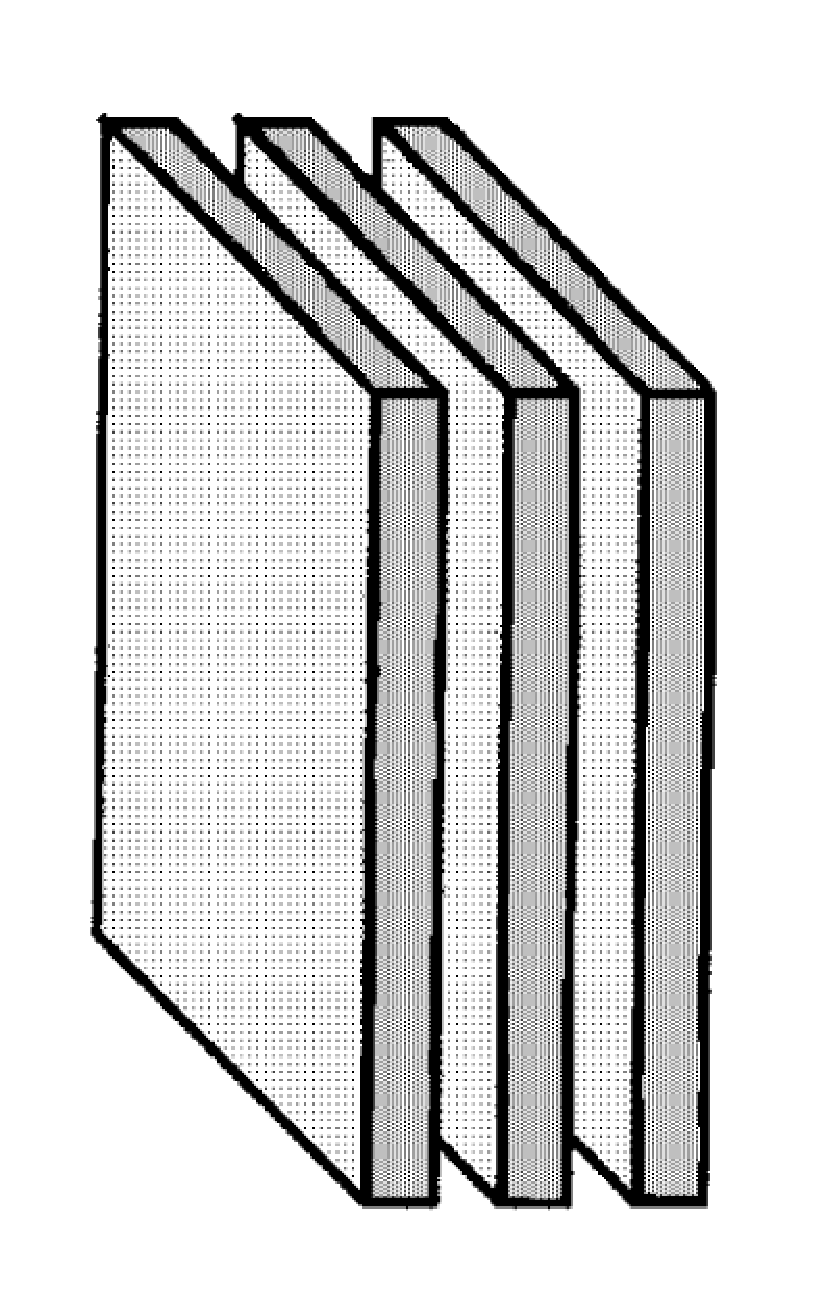
\includegraphics[width=\textwidth]{figures/einleitung/fig1}
    \end{subfigure}
    \begin{subfigure}[b]{0.15\textwidth}
        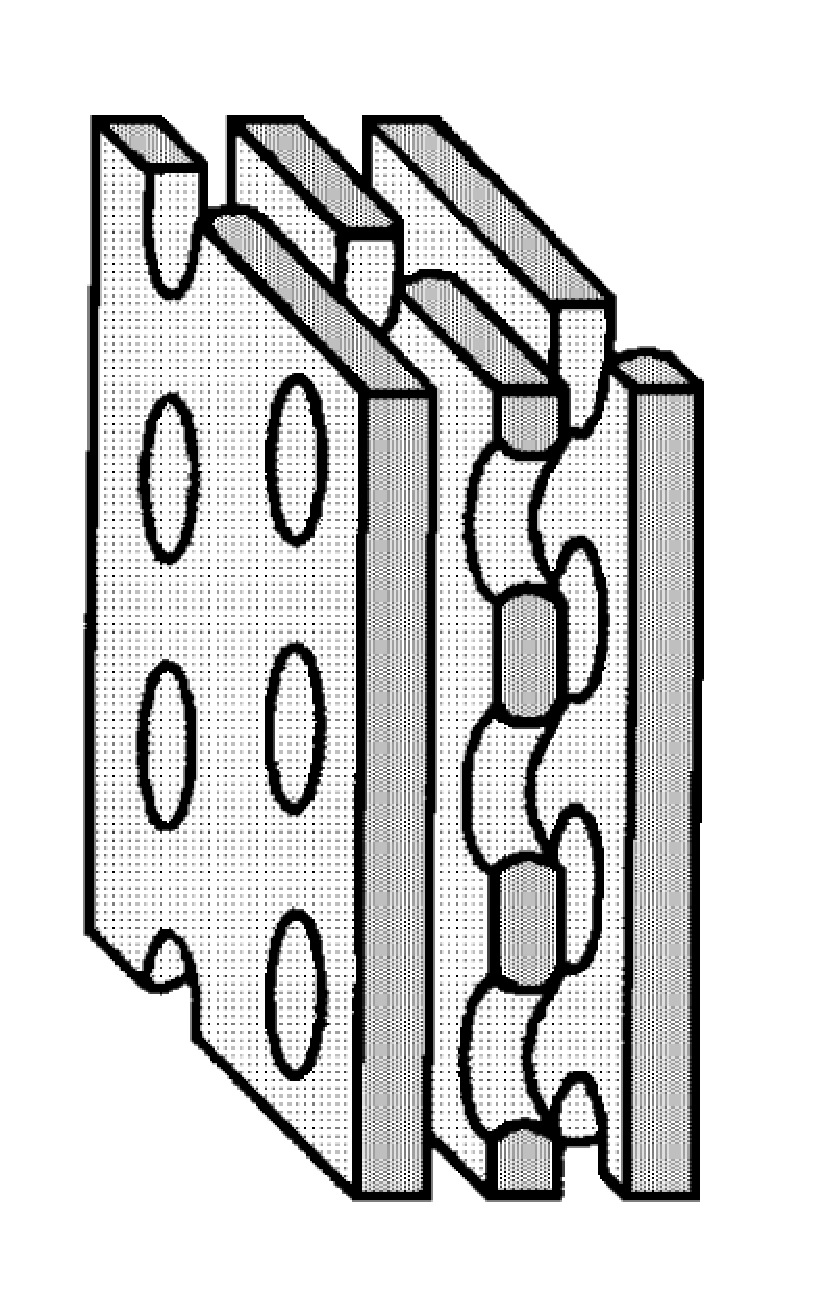
\includegraphics[width=\textwidth]{figures/einleitung/fig2}
    \end{subfigure}
    \begin{subfigure}[b]{0.15\textwidth}
        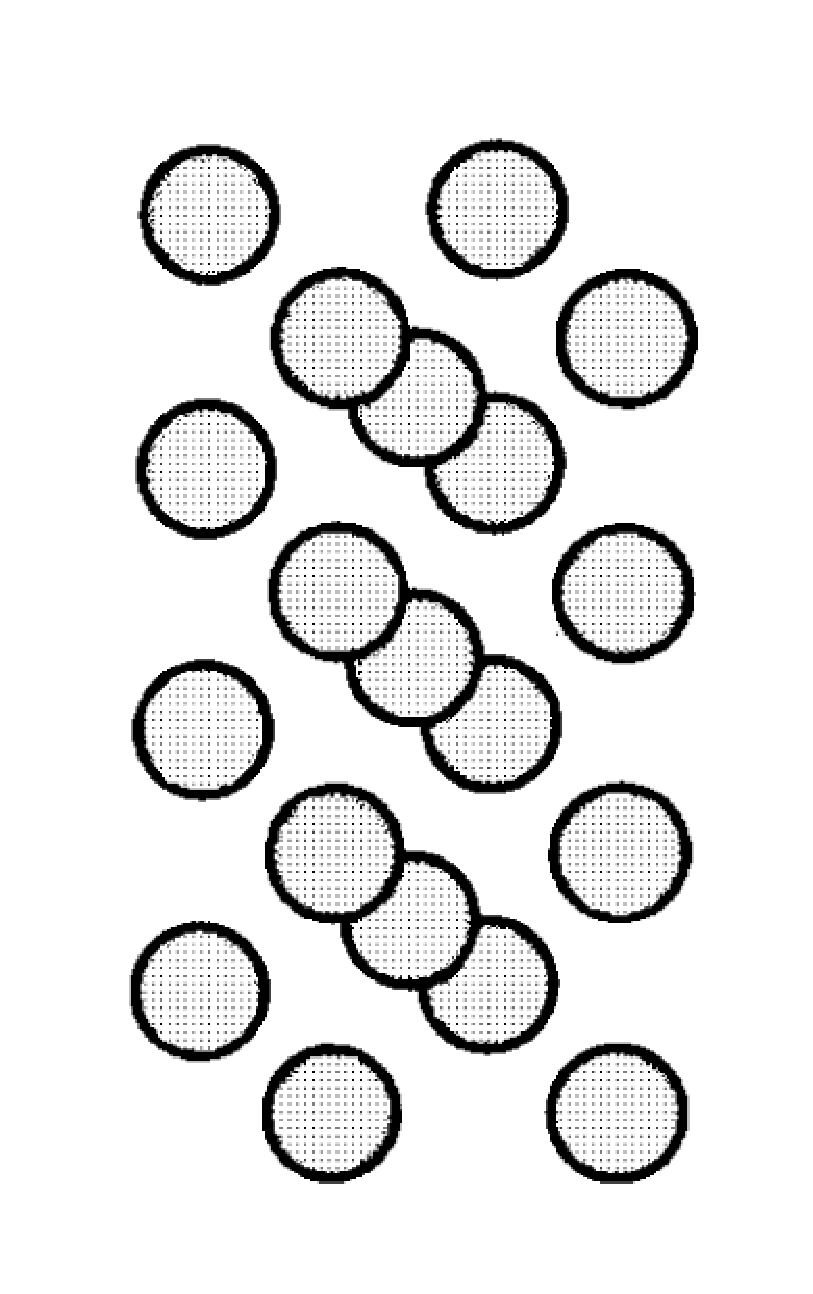
\includegraphics[width=\textwidth]{figures/einleitung/fig3}
    \end{subfigure}
    \begin{subfigure}[b]{0.15\textwidth}
        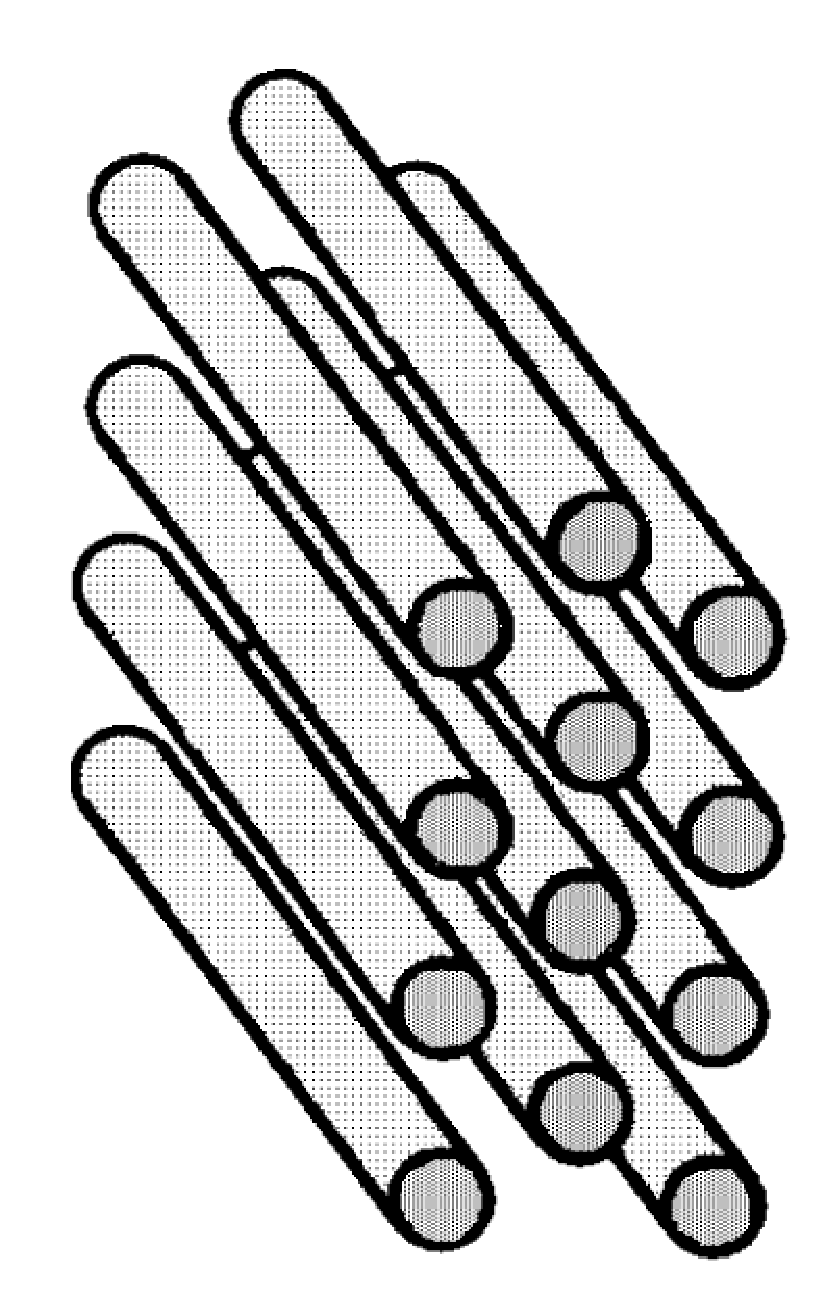
\includegraphics[width=\textwidth]{figures/einleitung/fig4}
    \end{subfigure}
    \begin{subfigure}[b]{0.15\textwidth}
        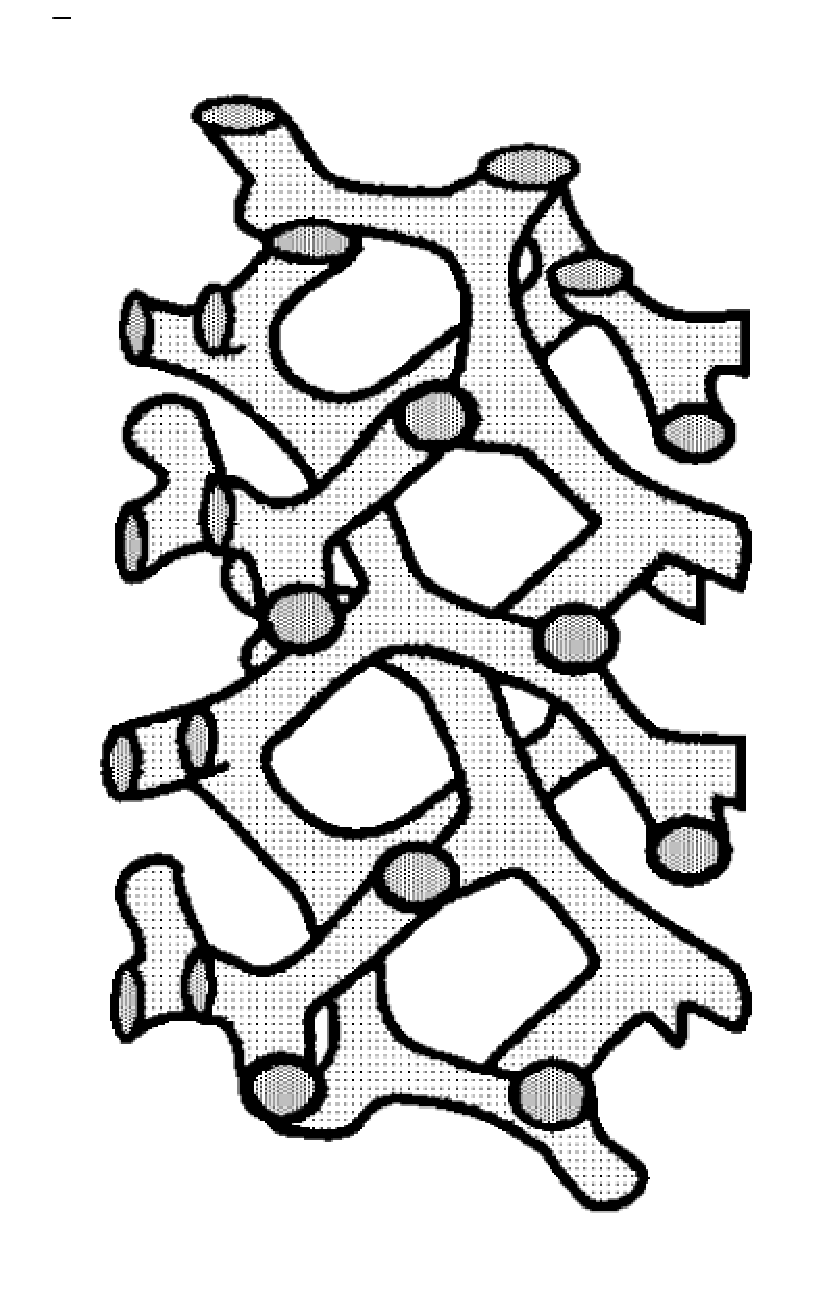
\includegraphics[width=\textwidth]{figures/einleitung/fig5}
    \end{subfigure}
    \caption[Verschiedene Phasen bei Diblockcopolymeren]{%
        Verschiedene Phasen bei Diblockcopolymeren, welche experimentell beobachtet wurden, wobei hierbei nur eine der beiden Monomer-Gattungen dargestellt wird.
        Diese heißen von links nach rechts: lamellar, perforiert-lamellar, sphärisch, zylindrisch, gyroid.
        Diese Abbildung wurde \cite[Figure 1.18]{Matsen:2006ud} entnommen.
    }
    \label{figure:phasen}
\end{figure}

\subsection*{Mathematische Modellierung} % (fold)

Als Grundlage für die \acl{scft} dient eine Modellierung der Polymere als frei bewegliche Ketten (\foreign{engl.}{ideal chain}).
Im Rahmen dieser Arbeit betrachten wir zwar nur die aus dem sogenannten stetigen Gaußschen Kettenmodell resultierende Theorie, erläutern aber zunächst ein diskretes Kettenmodell, welches eine Vorstufe des stetigen darstellt und die Idee dahinter verdeutlicht.
Eine deutlich ausführlichere und vor allem mathematisch begründete Einführung in diese Thematik findet man bei \textcites[Chapter 2]{Fredrickson:2006th}{rubinstein2003polymer}.

Im Folgenden betrachten wir eine nicht näher spezifizierte Volumenzelle und geben mit dem Vektor $\vec{r}$ eine Position in diesem Volumen an.

Das diskrete Modell stellt die Polymerkette als eine diskrete Kette von Partikeln dar, derart, dass aneinanderhängende Monomere ähnlich einem Scharnier frei beweglich sind.
Dabei werden Wechselwirkung zwischen benachbarten Monomeren berücksichtigt, während auf der Kette weit auseinanderliegende Partikel aber ignoriert werden.
Diese Wechselwirkungen können in \cref{figure:kettenmodelle} beispielsweise als Einschränkung des Winkels $\vartheta_9$ durch die gegenseitige Beeinflussung der Partikel $8, 9$ und $10$ auftreten.

Das stetige Gaußsche Kettenmodell, welches man unter anderem auch als stetigen Grenzfall des beschriebenen diskreten Modells erhält, hat sich als besonders nützlich erwiesen, sowohl bei analytischen als auch numerischen Betrachtungen.
Dabei wird die Polymerkette als stetige, linear elastische Faser aufgefasst und durch eine Kurve $\vec{r}(s)$ parametrisiert, wobei $s \in [0, 1]$ eine entlang der normalisierten Kontur der Kette verlaufende Variable ist.

\begin{figure}[tb]
    \centering
        \includestandalone[width=0.6\textwidth]{tikz/einleitung/chains}
    \caption[%
        Polymerkette in diskretem und Gaußschen Kettenmodell
    ]{%
        Schematische Darstellung einer Polymerkette im diskreten Kettenmodell (links) und im stetigen Gaußschen Kettenmodell (rechts).
        Abbildung reproduziert nach \cite[Figure 2.1 und 2.5]{Fredrickson:2006th}.
    }
    \label{figure:kettenmodelle}
\end{figure}

Sowohl das diskrete als auch das stetige Kettenmodell haben einen starken Bezug zur Stochastik, da sie sich auch als Random Walks beziehungsweise stochastische Prozesse auffassen lassen.
Dies stellt einen umfangreichen \enquote{Werkzeugkasten} zur Untersuchung dieser zur Verfügung.
Da die benötigten stochastischen Ausführungen und Herleitungen für diese Arbeit jedoch nebensächlich sind, belassen wir es bei diesen informalen Beschreibungen und widmen uns nun der darauf aufbauenden \ac{scft}.


\subsection*{Selbstkonsistente Feldtheorie} % (fold)

Bei der selbstkonsistenten Feldtheorie handelt es sich um ein weit verbreitetes theoretisches Modell der Physik um das Verhalten von Teilchen unter Einwirkung von Kräften, die durch Wechselwirkungen mit weiteren Teilchen auftreten, zu studieren und sie wird nicht nur im Zusammenhang mit Polymeren sondern zum Beispiel auch in der Thermodynamik oder Informatik verwendet.

Die Grundidee ist die folgende: in einem System vieler wechselwirkender Objekte kann die auf ein einzelnes Teilchen wirkende Gesamtkraft durch Mittelung aller Wechselwirkungen approximiert werden.
Diese gemittelten Einwirkungen werden als externes Feld aufgefasst und ignorieren dabei Fluktuationen, das heißt Veränderungen der wirkenden Kräfte durch das lokale Verhalten, beispielsweise Bewegungen, der einzelnen Teilchen.
Damit erreicht man effektiv die Reduktion eines Mehrkörperproblems auf ein Einkörperproblem und kann so das Verhalten eines solchen Systems untersuchen.

Dieses Prinzip lässt sich auch zur Untersuchung von Polymeren verwenden, da eine einzelne Polymerkette oftmals aus einer hohen vierstelligen Zahl von Atomen besteht und dadurch die Wechselwirkungen auf atomarem Level vernachlässigbar sind.
Aufbauend auf den beschriebenen Modellen, in diesem Fall dem stetigen Gaußschen Kettenmodell, kann so die statistische räumliche Ausrichtung von Polymerketten bestimmt werden.

Wir beschränken uns im Folgenden auf die Beschreibung der \ac{scft} für die inkompressible Schmelze eines AB-Diblockcopolymers und folgen dabei größtenteils den Ausführungen von \textcite{Matsen:1994bz,Stasiak:2011ba}.

Erneut wird eine einzelne Volumenzelle betrachtet, beispielsweise ein Würfel, welche selbst Teil eines größeren Systems sein kann.
Diese Zelle enthalte $n$ AB"=Diblockcopolymere, welche jeweils aus einem A-Block und einem B-Block bestehen, wobei diese wiederum aus $N_{\mathrm{A}}$ Monomeren vom Typ A respektive aus $N_{\mathrm{B}}$ Monomeren vom Typ B zusammengesetzt sind.
Der Polymerisationsgrad, das heißt die Gesamtanzahl an Monomeren in einem Polymer, ist durch $N = N_{\mathrm{A}} + N_{\mathrm{B}}$ gegeben.
Weiter bezeichne $f = N_{\mathrm{A}} / N$ den Anteil an A-Monomeren im gesamten Polymer.
Wie bei der Beschreibung des Gaußschen Modells ist $s \in [0, 1]$ eine normalisierte Distanz entlang der Kontur einer Polymerkette, wobei $s = 0$ und $s = 1$ den beiden Enden entspricht.

Als vereinfachende Annahmen sei die statistische Länge $a$ eines Monomers, auch Kuhn-Länge genannt, der beiden Monomer-Gattungen gleich und ein Monomer beider Gattungen nehme das selbe Volumen $1 / \rho_{0}$ ein.
Das Gesamtvolumen der Schmelze in dieser Zelle ist damit durch $V = n N / \rho_{0}$ gegeben.

Die wichtigsten Größen bei der \ac{scft} sind nun die Konzentrationen $\phi_{\mathrm{A}}(\vec{r})$ und $\phi_{\mathrm{B}}(\vec{r})$ der A- und B-Monomere an einer Position $\vec{r}$ in der betrachteten Zelle und die externen Felder $\omega_{\mathrm{A}}(\vec{r})$ und $\omega_{\mathrm{B}}(\vec{r})$, welche auf die jeweiligen Monomer-Gattungen wirken.

Als Ausgangspunkt für die Bestimmungen möglicher stabiler Anordnungen in der Polymerschmelze dient das sogenannte Freie-Energie-Funktional des Systems, genauer siehe \cite{Matsen:2006ud,Fredrickson:2006th}, welches für die freie Energie $F$ eines einzelnen Polymers die Form
\begin{equation}
\label{eq:freie_energie_funktional}
    \frac{F}{nk_{\mathrm{B}}T} = - \ln \frac{Q}{V} + \frac{1}{V} \int \chi N \phi_{\mathrm{A}}(\vec{r}) \phi_{\mathrm{B}}(\vec{r}) - \omega_{\mathrm{A}}(\vec{r}) \phi_{\mathrm{A}}(\vec{r}) - \omega_{\mathrm{B}}(\vec{r}) \phi_{\mathrm{B}}(\vec{r}) \diff \vec{r}
\end{equation}
hat, wobei $\chi$ der sogenannte Flory-Huggins-Wechselwirkungsparameter für die Wechselwirkungen zwischen den Monomeren vom Typ A und B und $k_{\mathrm{B}} T$ die thermische Energie ist.

Stabile Anordnungen der Polymerketten entsprechen Sattelpunkten des Freie-Energie-Funktionals bezüglich der Konzentrationen $\phi_{\mathrm{A}}$, $\phi_{\mathrm{B}}$ und der Felder $\omega_{\mathrm{A}}$ und $\omega_{\mathrm{B}}$.
Betrachtet man die Funktionalableitungen von $F$ bezüglich dieser Größen, dann bilden diese ein System von Gleichungen, kurz \ac{scft}-Gleichungen genannt, anhand derer die gesuchten Sattelpunkte bestimmt werden können.
Diese Gleichungen bestehen aus der Inkompressibilität der Schmelze
\begin{equation}
\label{eq:inkompressibilitaet}
    \phi_{\mathrm{A}}(\vec{r}) + \phi_{\mathrm{B}}(\vec{r}) = 1
\end{equation}%
sowie der Kopplung der Felder und der Konzentrationen durch
\begin{equation}
\label{eq:felder}
    % \begin{aligned}
        \omega_{\mathrm{A}}(\vec{r}) = \chi N \phi_{\mathrm{B}}(\vec{r}) + \xi(\vec{r}), \qquad
        \omega_{\mathrm{B}}(\vec{r}) = \chi N \phi_{\mathrm{A}}(\vec{r}) + \xi(\vec{r}),
    % \end{aligned}
\end{equation}%
wobei mit dem Lagrange-Multiplikator $\xi(\vec{r})$ die Inkompressibilität \cref{eq:inkompressibilitaet} erzwungen wird.
Weiter erhält man eine Darstellung der Konzentrationen in Form von
\begin{equation}
\label{eq:konzentrationen}
    % \begin{aligned}
        \phi_{\mathrm{A}}(\vec{r}) = \frac{V}{Q} \int_{0}^{f} q(\vec{r}, s) q^{\dagger}(\vec{r}, s) \diff s, \qquad
        \phi_{\mathrm{B}}(\vec{r}) = \frac{V}{Q} \int_{f}^{1} q(\vec{r}, s) q^{\dagger}(\vec{r}, s) \diff s,
    % \end{aligned}
\end{equation}%
wobei $Q = Q[\omega_{\mathrm{A}}, \omega_{\mathrm{B}}]$ die Partitionsfunktion (\foreign{engl.}{partition function}) eines einzelnen Polymers ist und durch
\begin{equation}
\label{eq:partitionsfunktion}
    Q = \int q(\vec{r}, 1) \diff \vec{r}
\end{equation}%
bestimmt wird.

Die in den Gleichungen \cref{eq:konzentrationen,eq:partitionsfunktion} auftretende Funktion $q(\vec{r}, s)$ wird als Vorwärts-Propagator bezeichnet und erfüllt die parabolische partielle Differentialgleichung
\begin{equation}
\label{eq:forward_propagator}
    \frac{\partial}{\partial s} q(\vec{r}, s) = \frac{a^{2}N}{6} \Delta q(\vec{r}, s) - \omega_{\alpha(s)}(\vec{r}) q(\vec{r}, s), \quad
    q(\vec{r}, 0) = 1.
\end{equation}
Analog wird $q^{\dagger}(\vec{r}, s)$ als Rückwärts-Propagator bezeichnet, da dieser eine ähnliche Differentialgleichung der Form
\begin{equation}
\label{eq:backward_propagator}
    -\frac{\partial}{\partial s}q^{\dagger}(\vec{r}, s) = \frac{a^{2}N}{6} \Delta q^{\dagger}(\vec{r}, s) - \omega_{\alpha(s)}(\vec{r}) q^{\dagger}(\vec{r}, s), \quad
    q^{\dagger}(\vec{r}, 1) = 1
\end{equation}%
erfüllt.
Die Abbildung $\omega_{\alpha(s)}$ ist dabei definiert als
\begin{equation}
    \omega_{\alpha(s)}(\vec{r}) = \begin{cases}
        \omega_{\mathrm{A}}(\vec{r}), & 0 \leq s < f,\\
        \omega_{\mathrm{B}}(\vec{r}), & f \leq s \leq 1.
    \end{cases}
\end{equation}

% Der Propagator $q(\vec{r}, s)$ repräsentiert das statistische Gewicht, im Wesentlichen eine nichtnormalisierte Wahrscheinlichkeit, dass man eine Polymerkette findet, welches an einem beliebigen Punkt des Volumens beginnt, und dessen Teilstück, das zur Konturvariable $s$ gehört, sich an der Position $\vec{r}$ befindet.
% Damit lässt sich die Anfangsbedingung $q(\vec r, 0) = 1$ so interpretieren, dass ein Polymer der Länge Null von den externen Feldern nicht beeinflusst wird.
% Der Rückwärts-Propagator hat die selbe Bedeutung, allerdings wird hierbei das andere Ende des Polymers festgehalten.

Je nachdem, welches Szenario betrachtet wird, entweder eine Volumenzelle innerhalb eines größeren Systems, oder eine Zelle, welche durch feste Wände begrenzt wird, erhält man verschiedene Randbedingungen an die beiden Differentialgleichungen.
Ersteres entspricht dabei periodischen Randbedingungen.

Ferner ist an dieser Stelle erwähnenswert, dass das Funktional der freien Energie \cref{eq:freie_energie_funktional} invariant ist bezüglich konstanter Verschiebungen der Felder $\omega_{\mathrm{A}}$ und $\omega_{\mathrm{B}}$, wie beispielsweise \cite{Ceniceros:2006is} entnommen werden kann.
Dies wird sich sowohl in der späteren theoretischen als auch numerischen Untersuchung als äußerst nützlich erweisen.


\subsection*{Einsatz numerischer Methoden} % (fold)

Es gibt verschiedene Ansätze, um die \ac{scft}-Gleichungen zu einem numerischen Verfahren zu verarbeiten.
Oftmals führen diese zu einem, dem nachfolgenden ähnlichen, iterativen Schema, welches Ähnlichkeiten mit einem Newton-Verfahren aufweist:

\begin{enumerate}[label={\itshape\roman*.},ref={\itshape\roman*}]
    \item Zunächst werden zufällig zwei externe Felder $\omega^{(0)}_{\mathrm{A}}$ und $\omega^{(0)}_{\mathrm{B}}$ generiert, um von vornherein auftretende Verzerrungen zu einem bestimmten Sattelpunkt zu verhindern.
    \item\label{enum:iterationsverfahren_punkt_2} Die Differentialgleichungen \cref{eq:forward_propagator,eq:backward_propagator} werden für die Felder $\omega^{(k)}_{\mathrm{A}}$ und $\omega^{(k)}_{\mathrm{B}}$ gelöst.
    \item Die Konzentrationen $\phi^{(k)}_{\mathrm{A}}$ und $\phi^{(k)}_{\mathrm{B}}$ werden durch die Gleichungen \cref{eq:partitionsfunktion,eq:konzentrationen} bestimmt.
    \item Diese Konzentrationen werden nun benutzt, um mittels den Gleichungen \cref{eq:felder} die zugehörigen Felder zu bestimmen.
    Aus diesen Feldern werden mit einem Mixing-Verfahren die neuen Felder $\omega^{(k+1)}_{\mathrm{A}}$ und $\omega^{(k+1)}_{\mathrm{B}}$ für die nächste Iteration erzeugt.
    Das Mixing dient dazu, die Konvergenz des Verfahrens sicherzustellen beziehungsweise zu verbessern.
    Typischerweise gehen hier die Inkompressibilität \cref{eq:inkompressibilitaet} und zurückliegende Iterationen ein.
    \item Wurde ein Sattelpunkt von \cref{eq:freie_energie_funktional} gefunden, so terminiert das Verfahren, ansonsten wird die Iteration ab \cref{enum:iterationsverfahren_punkt_2} fortgesetzt.
\end{enumerate}
%
Bei dem beschriebenen Verfahren stellen sich die folgenden beiden Schritte als besonders wichtig heraus, da sie maßgeblich die Laufzeit des Iterationsverfahren beeinflussen:
\begin{enumerate}[label={\itshape\roman*.}]
    \item das Lösungsverfahren für die Differentialgleichungen \cref{eq:forward_propagator} und \cref{eq:backward_propagator},
    \item das Mixing-Verfahren, mit dem iterativ neue Felder $\omega_{\mathrm{A}}$ und $\omega_{\mathrm{B}}$ bestimmt werden.
\end{enumerate}
%
Auf den zweiten Punkt, das Mixing-Verfahren, werden wir im Verlauf dieser Arbeit nicht weiter eingehen und stattdessen hier einige der verwendeten Ansätze erwähnen.
Da der Mixing-Schritt im Wesentlich als Konvergenzbeschleuniger des Iterationsverfahrens angedacht ist, lassen sich hierfür viele bekannte Verfahren der nichtlinearen Optimierung, aber auch aus anderen Bereichen, anwenden.
Dies reicht von einem Quasi-Newton-Verfahren \cite{Matsen:1994bz} bis zu Integrationsverfahren, wie zum Beispiel Runge-Kutta-Verfahren oder Mehrschrittverfahren.
Ein auf einem solchen Integrationsverfahren basierendes Mixing findet sich in \cite{Ceniceros:2006is}, ferner findet man darin auch ein auf einem CG-Verfahren aufbauendes Mixing.
Als besonders effektiver Ansatz hat sich das sogenannte Anderson-Mixing erwiesen, siehe die Arbeiten \cite{Thompson:2004um,Stasiak:2011ba}.
Dabei werden neue Felder durch Kombination der Felder vieler zurückliegender Iterationen gewonnen.
Weiter wurden in \cite{Drolet:1999bs} Verfahren ähnlich einer Picard-Iteration betrachtet.

Unser Hauptaugenmerk in dieser Arbeit liegt auf dem ersten Problem, dem wiederholten Lösen der parabolischen partiellen Differentialgleichung \cref{eq:forward_propagator}.
Da es, abhängig vom gewählten Mixing-Verfahren, oftmals eine Iterationsanzahl im dreistelligen Bereich oder höher benötigt, bis eine zufriedenstellende Genauigkeit bei der Sattelpunktgleichung erreicht ist, und damit insbesondere auch die partielle Differentialgleichung so oft gelöst werden muss, ist es wichtig, dass das Lösungsverfahren möglichst effizient ist.
Weiter darf zu Gunsten der Laufzeit aber auch nicht die Genauigkeit des Lösers vernachlässigt werden, da sich dies im Iterationsverfahren durch Instabilität und zusätzliche Iterationen niederschlagen kann.

Ähnlich wie beim Mixing-Schritt wurden bereits viele verschiedene Ansätze mit mehr oder weniger zufriedenstellenden Ergebnissen verfolgt.
Da es sich bei \cref{eq:forward_propagator} im Grunde um eine Diffusionsgleichung handelt, lassen sich gut bekannte Methoden, zum Beispiel ein Finite-Differenzen-Verfahren, anwenden.
So wird in \cite{Drolet:1999bs} ein Crank-Nicolson-Verfahren eingesetzt, wobei hierbei explizit der Laufzeit Vorrang gegenüber der Genauigkeit gegeben wurde.

\begin{figure}[tb]
    \centering
    \begin{subfigure}[b]{0.475\textwidth}
        \centering
        \includestandalone[width=1\textwidth]{tikz/einleitung/plot1}
        \caption{Felder}
    \end{subfigure}
    ~
    \begin{subfigure}[b]{0.475\textwidth}
        \centering
        \includestandalone[width=1\textwidth]{tikz/einleitung/plot2}
        \caption{Fourier-Koeffizienten}
    \end{subfigure}
    \caption[%
    Eindimensionales Beispiel einer stabilen Anordnung eines Diblockcopolymers
    ]{%
        Eindimensionales Beispiel einer stabilen Anordnung eines Diblockcopolymers, welche mittels \ac{scft} und Pseudospektralverfahren bestimmt wurde.
        Simuliert wurde auf einem Intervall der Länge $L = 10$ mit den relevanten Größen $f = 1/2$, $\chi N = 25$ und $a^{2} N / 6 = 10 / 3$.
        Monomer-Typ A entspricht den blauen und B dementsprechend den orangen Graphen.
        Die Fourier-Koeffizienten haben die Reihenfolge $\cos(2 \pi x), \sin(2 \pi x), \cos(4 \pi x), \dots$ und der konstante Anteil wurde vernachlässigt.
    }
    \label{figure:felder_nach_iterationsverfahren}
\end{figure}

Als guter Kompromiss zwischen Laufzeit und Genauigkeit haben sich Spektral- und Pseudospektralverfahren etabliert.
Erstere wurden von \textcite{Matsen:1994bz} erfolgreich eingesetzt, wobei hier erst das explizite Berücksichtigen der Symmetrien der zu erwartenden resultierenden Anordnung bei der Konstruktion des Spektralverfahrens zu annehmbaren Laufzeiten führt.
Die damit verwandten Pseudospektralverfahren kommen zwar nicht an die Genauigkeit der Spektralverfahren heran, können aber unter Ausnutzung der Struktur der partiellen Differentialgleichung massiv Laufzeit einsparen.
Dazu wird in \cite{Rasmussen:2002kt} der Differentialoperator mittels Operator-Splitting so zerlegt, dass man das Lösen der Differentialgleichung mittels schneller Fourier-Transformation im Wesentlichen auf komponentenweise Vektor-Multiplikationen zurückführt.
Das daraus resultierende Verfahren zweiter Ordnung wurde von \cite{GarciaCervera:2006uu,Ranjan:2007kl} auf unterschiedliche Weisen zu Verfahren vierter Ordnung erweitert, ohne signifikant Laufzeit einzubüßen.
Eine gute Übersicht über die meisten der hier genannten Methoden findet man bei \textcites[Section 3.6]{Fredrickson:2006th}{Audus:2013ep}.

Obwohl die Literatur zur \ac{scft} für Polymere verschiedenste Verfahren für das Lösen der partiellen Differentialgleichung bietet, ist ein Finite-Elemente-Ansatz basierend auf einer Raum-Zeit-Variationsformulierung unseres Wissens nach bisher nicht verfolgt worden.

Hier knüpfen wir an und betrachten das Problem, eine Lösung für die Differentialgleichung zu finden, losgelöst vom eigentlichen \ac{scft}-Iterationsverfahren, da der Berechnungsaufwand des in dieser Arbeit hergeleiteten Verfahrens eine Integration in das Iterationsverfahren im Rahmen dieser Arbeit unmöglich macht.
Die Grundidee ist die Verwendung eines Galerkin-Verfahrens für die Differentialgleichung mit anschließendem Aufsetzen eines Reduzierte-Basis-Ansatzes.
Für diesen ist es notwendig die Differentialgleichung zu parametrisieren, indem die in der Differentialgleichung auftretenden Felder in einem geeigneten Funktionensystem entwickelt werden.
Dieses sollte so gewählt werden, dass die Entwicklungskoeffizienten möglichst schnell abfallen.
Hierzu sei auf \cref{figure:felder_nach_iterationsverfahren} verwiesen, welche ein Felder-Paar von einem Iterationsdurchlauf und dessen Fourier-Koeffizienten zeigt.


\subsection*{Inhaltlicher Aufbau}

In \cref{chapter:grundlagen} werden zunächst die die funktionalanalytischen Grundlagen eingeführt beziehungsweise wiederholt, welche dann in \cref{chapter:propagator_differentialgleichung} verwendet werden um die parabolische partielle Differentialgleichung, welche im Rahmen dieser Einleitung bereits vorgestellt wurde, unter passenden Rahmenbedingungen zu formalisieren.
Weiter parametrisieren wir die Differentialgleichung und weisen unter bestimmten Bedingungen eine Regularität der Lösungen der Differentialgleichung vom Parameter nach.

Nachfolgend werden in \cref{chapter:galerkin} die ersten numerischen Grundlagen in Form des Petrov-Galerkin-Verfahrens gelegt und an einigen Beispiele analysiert, um dann darauf aufbauend in \cref{chapter:rbm} die Reduzierte-Basis-Methoden einzuführen und diese ebenfalls auf die in dieser Arbeit betrachtete Problemstellung anzuwenden.

Abschließend wird in \cref{chapter:ausblick} ein Résumé der Arbeit und daran anknüpfend ein Ausblick, welcher mögliche Ansatzpunkte für Verbesserungen und Weiterentwicklungen erläutert, gegeben.

% subsection aufbau_der_restlichen_arbeit (end)

% chapter einleitung (end)

    % -*- root: ../main.tex -*-

\documentclass[../main.tex]{subfiles}
\begin{document}

\chapter{Funktionalanalytische Grundlagen} % (fold)
\label{chapter:grundlagen}

Um die in der Einleitung beschriebenen parabolischen partiellen Differentialgleichungen theoretisch und numerisch untersuchen zu können, müssen wir zunächst ein robustes Grundgerüst schaffen.
Dies beginnen wir in diesem Kapitel mit der Einführung respektive Wiederholung der benötigten Grundlagen aus der Funktionalanalysis.
Dabei orientieren wir uns maßgeblich an den Arbeiten von \textcite{Dautray:1992by,Schweizer2013}, in welchen die nachfolgenden Ausführungen weit detaillierter zu finden sind.


\section{Bochner"=Räume} % (fold)
\label{section:bochner_raeume}

Bevor wir uns an die Herleitung einer Raum"=Zeit"=Variationsformulierung parabolischer partieller Differentialgleichungen begeben, müssen wir zunächst die zugrundeliegenden Funktionenräume einführen.
Hierbei konzentrieren wir uns auf die sogenannten \emph{Bochner"=Räume}, welche eine Verallgemeinerung der bekannten Lebesgue"=Räume $L_{p}$ auf Banachraum"=wertige Funktionen darstellen, schränken uns dabei aber stets auf den für uns relevanten Fall eines endlichen Zeitintervalls ein.
Weiter beschränken wir uns in dieser Arbeit auf die Betrachtung reeller Räume und Abbildungen, wobei ein Großteil der Aussagen auch für Strukturen über den komplexen Zahlen gilt.

Wir beginnen nun mit der folgenden Definition der Bochner"=Räume nach \cite[Definition XVIII.1.1]{Dautray:1992by}.

% TODO: eventuell nur auf L_2 beschränken.
\begin{Definition}
\label{definition:bochner_raum}
    Seien $X$ ein Banachraum und $- \infty < a < b < \infty$.
    Als \emph{Bochner"=Raum} $L_{2}(a, b; X)$ bezeichnen wir die Menge (der Äquivalenzklassen) $L_{2}$"=integrierbarer Funktionen $f \colon [a, b] \to X$, das heißt aller auf $[a, b]$ messbaren Funktionen mit
    \begin{equation}
        \norm{f}_{L_{2}(a, b; X)} := \left( \int_{a}^{b} \norm{f(t)}_{X}^{2} \diff t \right)^{1 / 2} < \infty.
    \end{equation}
    Ferner ist der \emph{Bochner"=Raum} $L_{\infty}(a, b; X)$ definiert als die Menge (der Äquivalenzklassen) der für fast alle $t \in [a, b]$ wesentlich beschränkten Funktionen, also aller messbaren Funktionen $f \colon [a, b] \to X$ mit
    \begin{equation}
        \norm{f}_{L_{\infty}(a, b; X)} := \esssup_{t \in [a, b]} \norm{f(t)}_{X} < \infty.
    \end{equation}
\end{Definition}

\begin{Lemma}
\label{lemma:bochnerraum_ist_banachraum_bzw_hilbertraum}
    Der Bochner-Raum $L_{2}(a, b; X)$ ist ein Banachraum.
    Ist ferner $H$ ein Hilbertraum, so auch $L_{2}(a, b; H)$ mit dem Skalarprodukt
    \begin{equation}
        \skp{u}{v}{L_{2}(a, b; H)} := \int_{a}^{b} \skp{u(t)}{v(t)}{H} \diff t, \quad \text{für}~u,v \in L_{2}(a, b; H).
    \end{equation}

    \begin{Beweis}
        Die erste Aussage findet sich in \cite[Proposition XVIII.1.1]{Dautray:1992by}, die zweite in \cite[Abschnitt 1.1.3]{Lions:1972tg}.
    \end{Beweis}
\end{Lemma}

Weiter können wir für Funktionen aus einem Bochner"=Raum eine Zeitableitung definieren, hier nach \cites[471]{Dautray:1992by}[Definition 10.6]{Schweizer2013}.

\begin{Definition}%[Zeitableitung]
\label{definition:zeitableitung}
    Seien $X$ und $Y$ Banachräume mit stetiger Einbettung $X \hookrightarrow Y$ und sei $u \in L_{2}(a, b; X)$.
    Existiert ein $v \in L_{2}(a, b; Y)$ mit
    \begin{equation}
        \int_{a}^{b} v(t) \varphi(t) \diff t = - \int_{a}^{b} u(t) \varphi'(t) \diff t, \quad \fa \varphi \in \mathcal C^{\infty}_{0}((a, b), \mathbb{R}),
    \end{equation}
    so bezeichnen wir diese distributionelle Ableitung $u_{t} := v$ als \emph{Zeitableitung} von $u$.
\end{Definition}

\begin{Bemerkung}
    Der einfacheren Notation wegen werden wir die beiden Schreibweisen $u_{t}$ und $u'$ für die Zeitableitung verwenden.
\end{Bemerkung}

Obige Definition einer Zeitableitung ermöglicht die Definition der Bochner"=Sobolev"=Räume.
Wir beschränken uns hier auf den für uns relevanten Raum erster Ordnung, siehe \cite[Section 5.9.2]{evans2010partial}.

\begin{Definition}
\label{definition:bochner_sobolev_raum}
    Sei $X$ ein Banachraum.
    Als \emph{Bochner"=Sobolev"=Raum} erster Ordnung definieren wir den Raum
    \begin{equation}
        H^{1}(a, b; X) := \Set{u \in L_{2}(a, b; X) \given u' \in L_{2}(a, b; X)}.
    \end{equation}
\end{Definition}

Ferner gilt eine zu \cref{lemma:bochnerraum_ist_banachraum_bzw_hilbertraum} analoge Aussage auch für Bochner"=Sobolev"=Räume.
Da wir im Zuge dieser Arbeit ausschließlich mit Hilberträumen arbeiten werden, wird sich das folgende Konstrukt als grundlegend erweisen.
Die nachfolgende Definition ist eine leichte Abwandlung von \cite[Abschnitt 10.2]{Schweizer2013}.

\begin{Definition}
\label{definition:gelfand_tripel}
    Seien $V$ und $H$ separable Hilberträume mit den Dualräumen $V'$ und $H'$.
    Weiter sei die Einbettung $V \denseinclusion H$ dicht und stetig.
    Durch die Identifikation $H \cong H'$ erhalten wir das sogenannte \emph{Gelfand"=Tripel} $V \denseinclusion H \denseinclusion V'$, wobei die zweite Inklusionen ebenfalls eine dichte stetige Einbettung ist.
\end{Definition}

\begin{Bemerkung}
\label{bemerkung:skalarprodukte_und_duality_pairing}
    Es seien $\skp{\blank}{\blank}{V}$ und $\skp{\blank}{\blank}{H}$ die Skalarprodukte auf $V$ respektive $H$.
    Weiter verwenden wir die Schreibweise $\skp{\blank}{\blank}{V' \times V}$ auch für die duale Paarung auf $V' \times V$, welche die eindeutige stetige Fortsetzung von $\skp{\blank}{\blank}{H}$ ist.
    Dadurch gilt insbesondere
    \begin{equation}
        \skp{u}{v}{V' \times V} = \skp{u}{v}{H}, \quad \fa u \in H, v \in V.
    \end{equation}
\end{Bemerkung}

Mit Hilfe dieser Gelfand"=Tripel können wir nun die Räume definieren, welche wir letztendlich für die schwache Formulierung parabolischer partieller Differentialgleichungen benutzen werden.
Dies geschieht analog zu \cite[Definition XVIII.2.4]{Dautray:1992by}.

\begin{Definition}
\label{definition:bochner_raum_W}
    Sei $V \denseinclusion H \denseinclusion V'$ ein Gelfand"=Tripel.
    Wir definieren den Raum
    \begin{equation}
        W(a, b; V, V') := \Set{u \in L_{2}(a, b; V) \given u' \in L_{2}(a, b; V')},
    \end{equation}
    wobei $u'$ im Sinne von \cref{definition:zeitableitung} zu verstehen ist.
    Es gilt ferner
    \begin{equation}
        W(a, b; V, V') = L_{2}(a, b; V) \cap H^{1}(a, b; V').
    \end{equation}
\end{Definition}

Weiter können wir diesem Raum ein Skalarprodukt und damit auch eine Norm zuordnen.
Dies liefert die folgende Aussage.

\begin{Lemma}
\label{lemma:bochner_W_ist_hilbertraum}
    Versehen wir $W(a, b; V, V')$ mit dem Skalarprodukt
    \begin{equation}
        \skp{u}{v}{W(a, b; V, V')} := \skp{u}{v}{L_{2}(a, b; V)} + \skp{u'}{v'}{L_{2}(a, b; V')}
    \end{equation}
    und der dadurch induzierten Norm
    \begin{equation}
        \norm{u}_{W(a, b; V, V')} = \left( \norm{u}_{L_{2}(a, b; V)}^{2} + \norm{u'}_{L_{2}(a, b; V')}^{2} \right)^{1/2},
    \end{equation}
    so ist $W(a, b; V, V')$ ein Hilbertraum.

    \begin{Beweis}
        Ein Beweis findet sich in \cite[Proposition XVIII.2.6]{Dautray:1992by}.
    \end{Beweis}
\end{Lemma}

Da die von uns betrachteten parabolischen partiellen Differentialgleichungen jeweils mit Anfangsbedingungen versehen sein werden, müssen wir an dieser Stelle klären, in welchem Sinne diese zu verstehen sind.
Dies führt zum sogenannten Spursatz, welchen wir durch die folgende Einbettungsaussage erhalten.

\begin{Satz}
\label{satz:bochner_raum_W_stetige_einbettung_C0}
    Seien $V \denseinclusion H \denseinclusion V'$ ein Gelfand"=Tripel und $a, b \in \mathbb{R}$.
    Ferner sei $\mathcal C([a, b]; H)$ die Menge aller stetigen Funktionen $f \colon [a, b] \to H$.
    Dann ist die Einbettung
    \begin{equation}
        W(a, b; V, V') \hookrightarrow \mathcal C([a, b], H)
    \end{equation}
    stetig.
    Insbesondere stimmt jedes $u \in W(a, b; V, V')$ fast überall mit einer stetigen Funktion aus $\mathcal C([a, b], H)$ überein.

    \begin{Beweis}
        Siehe \cites[Theorem XVIII.2.1]{Dautray:1992by}[Theorem 10.9]{Schweizer2013}.
    \end{Beweis}
\end{Satz}

\begin{Korollar}[Spursatz]
\label{korollar:spursatz}
    Seien $a, b \in \mathbb{R}$ und $u \in W(a, b; V, V')$.
    Dann sind die \emph{Spuren} $u(a), u(b) \in H$ wohldefiniert.

    \begin{Beweis}
        Ergibt sich als direkte Folgerung aus \cref{satz:bochner_raum_W_stetige_einbettung_C0}, siehe auch \cite[Remark XVIII.2.4]{Dautray:1992by}.
    \end{Beweis}
\end{Korollar}

Ferner erhalten wir aus obiger Einbettungsaussage auch das folgende Ergebnis, welches im Rahmen der Betrachtung linearer Evolutionsgleichungen benötigt wird.

% TODO: Beispiel?
\begin{Korollar}
\label{korollar:einbettungskonstante_M_e}
    Seien $a, b \in \mathbb{R}$.
    Die Einbettungskonstante
    \begin{equation}
        \label{eq:einbettungskonstante_M_e}
        \gamma_{e} := \sup_{\substack{u\in W(a, b; V, V')\\u \neq 0}} \frac{\norm{u(a)}_{H}}{\norm{u}_{W(a, b; V, V')}}
    \end{equation}
    ist gleichmäßig beschränkt in der Wahl $V \hookrightarrow H$ und hängt nur im Fall $b \to a$ von $b$ ab.

    \begin{Beweis}
        Siehe \cites[Section 5]{Schwab:2009ec}[Beweis zu Theorem XVIII.2.1]{Dautray:1992by}.
    \end{Beweis}
\end{Korollar}
%
\newglossaryentry{sym:einbettungskonsanten_gamma_e}{
    sort={kEinbettungskonstante_gamma_e},
    name={$\gamma_{e}$},
    description={Einbettungskonstante, siehe \cref{korollar:einbettungskonstante_M_e}},
    type=symbolslist
}

Abschließen wollen wir diesen Abschnitt mit einer alternativen Charakterisierung der hier betrachteten Bochner"=Räume als Tensor"=Produkt, welche erst bei der numerischen Umsetzung in \cref{chapter:galerkin} relevant wird.

\begin{Satz}
\label{satz:bochner_sobolev_raum_als_tensorprodukt}
    Seien $V$ ein Hilbertraum und $a, b \in \mathbb{R}$ mit $a < b$.
    Dann ist der Bochner"=Sobolev"=Raum $H^{m}(a, b; V)$, $m \in \Set{0, 1}$, isometrisch isomorph zum Hilbertraum"=Tensorprodukt $H^{m}([a, b]) \otimes V$, kurz
    \begin{equation}
        H^{m}(a, b; V) \cong H^{m}([a, b]) \otimes V.
    \end{equation}

    \begin{Beweis}
        Siehe \cite[Theorem 12.6.1, Theorem 12.7.1]{Aubin:2000un} für einen ausführlichen Nachweis.
    \end{Beweis}
\end{Satz}


\section{Lineare Evolutionsgleichungen} % (fold)
\label{section:lineare_evolutionsgleichungen}

Nach der Einführung der benötigten Funktionenräume wenden wir uns nun den linearen Evolutionsgleichungen, einer bestimmten Unterart parabolischer partieller Differentialgleichungen, zu.
Wir orientieren uns hierbei an \textcite{Lions:1971wp}, \textcite{Schwab:2009ec} sowie \textcite{Urban:2014kg},
definieren den Begriff der linearen Evolutionsgleichungen, leiten eine schwache Formulierung her und weisen abschließend nach, dass diese korrekt gestellt ist.

Um den Begriff der linearen Evolutionsgleichungen definieren zu können, müssen wir zunächst die richtigen Rahmenbedingungen schaffen.
Sei $V \denseinclusion H \denseinclusion V'$ ein Gelfand-Tripel im Sinne von \cref{definition:gelfand_tripel}, das heißt, $V$ und $H$ seien separable Hilberträume und die Inklusionen seien jeweils dicht und stetig.
Weiter seien $0 < T < \infty$ und $I := [0, T]$.
Wir betrachten nun eine Familie $\Set{A(t) \in \mathcal L(V, V')}_{t \in I}$ von stetigen linearen Operatoren.
Nach dem Rieszschen Darstellungssatz, genauer siehe \cite[Theorem \S{}22.1]{Halmos:1957vd}, können wir diesen Operatoren eine Familie von Bilinearformen $\Set{a(\blank, \blank; t) \in \mathcal L(V \times V, \mathbb{R})}_{t \in I}$ zuordnen, wobei diese durch
\begin{equation}
    \skp{A(t)\eta}{\zeta}{V' \times V} = a(\eta, \zeta; t), \quad \fa \eta, \zeta \in V,
\end{equation}
induziert werden.

Wie wir später sehen werden, stellt die nachfolgende Annahme sicher, dass die auf diesen Operatoren aufbauenden linearen Evolutionsgleichungen gewisse wünschenswerte Eigenschaften wie Lösbarkeit und Eindeutigkeit dieser Lösung besitzen.

% TODO: für fast alle t besser einbauen
\begin{Annahme}
\label{annahme:eigenschaften_der_bilinearform_a}
    Die Familie $\Set{a(\blank, \blank; t) \in \mathcal L(V \times V, \mathbb{R})}_{t \in I}$ von Bilinearformen erfülle die folgenden Eigenschaften:
    \leavevmode
    \begin{thmenumerate}
        \item \emph{Messbarkeit:} die Abbildung $I \ni t \mapsto a(\eta, \zeta; t)$ sei messbar für alle $\eta, \zeta \in V$.
        \item \emph{Stetigkeit:}
        es existiere ein $0 < \gamma_{a} < \infty$ mit
        \begin{equation}
            \label{eq:eigenschaften_der_bilinearform_a:stetigkeit}
            \abs{a(\eta, \zeta; t)} \leq \gamma_{a} \norm{\eta}_{V} \norm{\zeta}_{V} \quad \fa \eta, \zeta \in V \text{ und fast alle } t \in I.
        \end{equation}
        \item \emph{G\r{a}rding-Ungleichung:}
        Es existieren $\alpha > 0$ und $\lambda \geq 0$ mit
        \begin{equation}
            \label{eq:eigenschaften_der_bilinearform_a:garding}
            a(\eta, \eta; t) + \lambda \norm{\eta}_{H}^{2} \geq \alpha \norm{\eta}_{V}^{2} \quad \fa \eta \in V \text{ und fast alle } t \in I.
        \end{equation}
    \end{thmenumerate}
\end{Annahme}
%
\newglossaryentry{sym:stetigkeitskonstante_gamma_a_b}{
    sort={kStetigkeitskonstanten},
    name={$\gamma_{a}$, $\gamma_{b}$},
    description={Stetigkeitskonstanten},
    type=symbolslist
}

Für den Rest dieses Abschnitts nehmen wir stets an, dass die obige Annahme erfüllt ist.
Diese Vorarbeit erlaubt uns nun die nachfolgende Definition.

\begin{Definition}
\label{definition:lineare_evolutionsgleichung}
    Seien $g \in L_{2}(I; V')$ ein \emph{Quellterm} und $u_{0} \in H$ ein \emph{Anfangswert}.
    Als \emph{lineare Evolutionsgleichung} bezeichnen wir die parabolische partielle Differentialgleichung
    \begin{equation}
        \label{eq:lineare_evolutionsgleichung}
        \left\{
        \begin{aligned}
            u_{t}(t) + A(t) u(t) &= g(t)     \quad&&\text{in}~V', \quad \text{für fast alle}~t \in I, \\
            u(0) &= u_{0}                    \quad&&\text{in}~H.
        \end{aligned}
        \right.
    \end{equation}
    % wobei die  Operatorfamilie $\Set{A(t) \in \mathcal L(V, V')}_{t \in I}$ wie oben gegeben sei.
\end{Definition}

Darauf aufbauend leiten wir als nächstes eine Raum-Zeit-Variationsformulierung für \cref{eq:lineare_evolutionsgleichung} her.
Dazu benötigen wir geeignete Ansatz- und Testfunktionenräume, wofür die im vorherigen Abschnitt eingeführten Bochner-Räume verwendet werden.

\begin{Definition}
\label{definition:ansatz_und_testraum}
    Den \emph{Ansatzfunktionenraum} $\mathcal X$ definieren wir als den Hilbertraum
    \begin{equation}
    \label{eq:ansatzraum_X}
        \mathcal X := W(I; V, V') = L_{2}(I; V) \cap H^{1}(I; V')
    \end{equation}
    mit dem Skalarprodukt
    \begin{equation}
    \label{eq:ansatzraum_skalarprodukt}
        \skp{u}{v}{\mathcal X} := \skp{u}{v}{L_{2}(I; V)} + \skp{u'}{v'}{L_{2}(I; V')}.
    \end{equation}
    Der \emph{Testfunktionenraum} $\mathcal Y$ sei als Produkt der beiden Hilberträume $\mathcal Y_{1} := L_{2}(I; V)$ und $\mathcal Y_{2} := H$ definiert als
    \begin{equation}
    \label{eq:testraum_Y}
        \mathcal Y := \mathcal Y_{1} \times \mathcal Y_{2} = L_{2}(I; V) \times H
    \end{equation}
    mit Skalarprodukt
    \begin{equation}
        \label{eq:testraum_skalarprodukt}
        \skp{u}{v}{\mathcal Y} := \skp{u_{1}}{v_{1}}{L_{2}(I; V)} + \skp{u_{2}}{v_{2}}{H}, \quad  u = (u_{1}, u_{2}), v = (v_{1}, v_{2}) \in \mathcal Y.
    \end{equation}
\end{Definition}

Um nun aus~\cref{eq:lineare_evolutionsgleichung} eine schwache Formulierung zu erhalten, \enquote{multiplizieren} wir die lineare Evolutionsgleichung mit $v = (v_{1}, v_{2}) \in \mathcal Y$ und integrieren anschließend im Ort als auch über das Zeitintervall $I = [0, T]$.
% Dadurch erhalten wir die nachfolgende Raum"=Zeit"=Variationsformulierung.

\begin{Definition}
\label{definition:absktrakte_raum_zeit_formulierung}
    Seien $\mathcal X$ und $\mathcal Y$ wie in~\cref{eq:ansatzraum_X,eq:testraum_Y}, $g \in L_{2}(I; V')$ ein Quellterm und $u_{0} \in H$ ein Anfangswert.
    Als \emph{Raum"=Zeit"=Variationsformulierung} der linearen Evolutionsgleichung~\cref{eq:lineare_evolutionsgleichung} bezeichnen wir das folgende Problem:
    \begin{equation}
        \label{eq:absktrakte_raum_zeit_formulierung}
        \text{Finde } u \in \mathcal X \text{ mit} \quad b(u, v) = f(v) \quad \fa v \in \mathcal Y.
    \end{equation}
    Dabei sei die Bilinearform $b \colon \mathcal X \times \mathcal Y \to \mathbb{R}$ durch
    \begin{equation}
        \label{eq:absktrakte_raum_zeit_formulierung:lhs}
        b(u, v) := \int_{I} \left[   \skp{u_{t}(t)}{v_{1}(t)}{V' \times V} + a(u(t), v_{1}(t); t)  \right] \diff t + \skp{u(0)}{v_{2}}{H}
    \end{equation}
    definiert und das Funktional $f \colon \mathcal Y \to \mathbb{R}$ durch
    \begin{equation}
        \label{eq:absktrakte_raum_zeit_formulierung:rhs}
        f(v) := \int_{I} \skp{g(t)}{v_{1}(t)}{V' \times V} \diff t + \skp{u_{0}}{v_{2}}{H}.
    \end{equation}
\end{Definition}

\begin{Bemerkung}
    Die Anfangswertbedingung $u(0) = u_{0}$ in $H$ ist wegen \cref{korollar:spursatz} wohldefiniert.
\end{Bemerkung}

Es bleibt nun zu zeigen, welche Bedingungen hinreichend sind, damit obige Raum"=Zeit"=Variationsformulierung \emph{korrekt gestellt} ist.
Dazu definieren wir zunächst, was wir darunter verstehen wollen und greifen dazu auf die Definition nach \textcite{hadamard1902problemes} zurück.

\begin{Definition}[Hadamard]
\label{definition:sachgemaess_gestellt_nach_hadamard}
    Seien $X$ und $Y$ zwei Hilberträume, $a \in \mathcal L(X \times Y, \mathbb{R})$ eine stetige Bilinearform und $f \in Y'$ ein stetiges lineares Funktional.
    Sei weiter ein abstraktes Variationsproblem gegeben durch:
    \begin{equation}
    \label{eq:hadamard_variationsproblem}
        \text{Finde } u \in X \text{ mit} \quad a(u, v) = f(v) \quad \fa v \in Y.
    \end{equation}
    Wir nennen dieses \emph{korrekt gestellt}, wenn eine eindeutige Lösung $u \in X$ existiert und diese eine a priori-Abschätzung der Form
    \begin{equation}
    \label{eq:hadamard_abschaetzung}
        \norm{u}_{X} \leq c \norm{f}_{Y'} \quad \fa f \in Y'
    \end{equation}
    mit einer von $f$ unabhängigen Konstante $c > 0$ erfüllt.
\end{Definition}

Um dies für die Raum"=Zeit"=Variationsformulierung \cref{eq:absktrakte_raum_zeit_formulierung} nachzuweisen, werden wir indirekt auf den nachfolgenden wichtigen Satz zurückgreifen.
Dieser findet sich in dieser oder ähnlicher Form bei \textcites[Theorem 2.1]{Babuska:1971fx}[Theorem 5.2.1]{Aziz:1972wf}[Theorem \S{}3.3.6]{Braess:2007wm}.

\begin{Satz}[Banach-Ne{\v c}as-Babu{\v s}ka-Theorem]
\label{satz:bnb_theorem}
    Seien $X$ und $Y$ zwei Hilberträume.
    Eine beschränkte lineare Abbildung $A \colon X \to Y'$ ist genau dann ein Isomorphismus, das heißt stetig invertierbar, wenn die zugehörige Bilinearform $a \colon X \times Y \to \mathbb{R}$ die folgenden Bedingungen erfüllt:
    \begin{thmenumerate}
        \item \label{satz:bnb_theorem:stetig}
        \emph{Stetigkeit:}
        Es existiert eine Konstante $0 < \gamma < \infty$ mit
        \begin{equation}
            \abs{a(u, v)} \leq \gamma \norm{u}_{X} \norm{v}_{Y} \quad \fa u \in X,~v\in Y.
        \end{equation}
        \item \label{satz:bnb_theorem:inf_sup_bedingung}
        \emph{Inf-sup-Bedingung:}
        Es existiert eine Konstante $\beta > 0$ mit
        \begin{equation}
            \infsup{u \in X}{v \in Y} \frac{a(u, v)}{\norm{u}_{X} \norm{v}_{Y}} \geq \beta.
        \end{equation}
        \item \label{satz:bnb_theorem:surjektiv}
        \emph{Surjektivität:}
        Zu jedem $v \in Y$, $v \neq 0$, existiert ein $u \in X$ mit
        \begin{equation}
            a(u, v) \neq 0.
        \end{equation}
    \end{thmenumerate}
    Gelten die drei Bedingungen und ist weiter ein Funktional $f \in Y'$ gegeben, dann existiert eine eindeutige Lösung $\hat u \in X$ mit
    \begin{equation}
        a(\hat u, v) = f(v) \quad \fa v \in Y
    \end{equation}
    und es gilt
    \begin{equation}
        \norm{\hat u}_{X} \leq \frac{1}{\beta} \norm{f}_{Y'}.
    \end{equation}
\end{Satz}

\begin{Bemerkung}
\label{bemerkung:bnb_theorem_inf_sup_statt_surjektiv}
    Nach \cite[Remarks, S. 117]{Aziz:1972wf} kann die Surjektivitätsbedingung \cref{satz:bnb_theorem:surjektiv} durch eine weitere inf"=sup"=Bedingung ersetzt werden, denn existiert ein $\beta' > 0$ mit
    \begin{equation}
        \infsup{v \in Y}{u \in X} \frac{a(u, v)}{\norm{u}_{X} \norm{v}_{Y}} \geq \beta',
    \end{equation}
    dann gilt insbesondere auch \cref{satz:bnb_theorem:surjektiv}.
\end{Bemerkung}

Für das abstrakte Raum"=Zeit"=Variationsproblem \cref{eq:absktrakte_raum_zeit_formulierung} wurde für die hier vorliegenden Rahmenbedingungen bereits von \textcite[Section XVIII.3]{Dautray:1992by} nachgewiesen, dass es sich um ein korrekt gestelltes Problem handelt.
Ein alternativer Beweis, welcher die Bedingungen des \acl{bnb}s nachweist und weiter explizite Schranken für die Stetigkeitskonstante $\gamma_{b}$ und die inf"=sup"=Konstante $\beta$ der Bilinearform $b$ aus \cref{eq:absktrakte_raum_zeit_formulierung:lhs} liefert, wurde von \textcite{Schwab:2009ec} geführt.
Wir wiederholen die Kernaussage \cite[Theorem 5.1]{Schwab:2009ec} und verweisen für einen ausführlichen Beweis auf \cite[Appendix A]{Schwab:2009ec}.

\begin{Satz}
\label{satz:ss09:theorem51}
    Seien $\mathcal X$ und $\mathcal Y$ wie in \cref{eq:ansatzraum_X,eq:testraum_Y} und sei $\Set{a(\blank, \blank; t) \in \mathcal L (V \times V)}_{t \in I}$ eine Familie von Bilinearformen, welche \cref{annahme:eigenschaften_der_bilinearform_a} erfüllt.
    Dann ist das Raum"=Zeit"=Variationsproblem \cref{eq:absktrakte_raum_zeit_formulierung} korrekt gestellt, das heißt, für alle $f \in \mathcal Y'$ existiert eine eindeutige Lösung $u \in \mathcal X$ so, dass
    \begin{equation}
        b(u, v) = f(v) \quad \fa v \in \mathcal Y
    \end{equation}
    gilt.
    Ferner existiert eine von $f$ unabhängige Konstante $\beta > 0$ mit
    \begin{equation}
        \norm{u}_{\mathcal X} \leq \frac{1}{\beta} \norm{f}_{\mathcal Y'}.
    \end{equation}
\end{Satz}

Weiter wollen wir im nachfolgenden Korollar die bereits angesprochenen Schranken für die Stetigkeitskonstante $\gamma_{b}$ und die inf"=sup"=Konstante $\beta$ der Bilinearform $b$ angeben.

% TODO: Beispiel?

\begin{Korollar}
\label{korrolar:ss09:theorem51_abschaetzungen}
    Unter den gleichen Voraussetzungen wie in \cref{satz:ss09:theorem51} und der Bedingung, dass die Bilinearformen $\Set{a(\blank, \blank; t)}_{t \in I}$ die G\aa{}rding-Ungleichung mit $\lambda = 0$ erfüllen, gilt
    \begin{equation}
        \label{eq:ss09:theorem51_abschaetzungen:lambda_null:stetig}
        \gamma_{b}  \leq \sqrt{2 \max\Set{1, \gamma_{a}^{2}} + \gamma_{e}^{2}}
    \end{equation}
    und
    \begin{equation}
        \label{eq:ss09:theorem51_abschaetzungen:lambda_null:inf_sup}
        \beta  \geq \frac{\min\Set{\alpha \gamma_{a}^{-2}, \alpha}}{\sqrt{2 \max \Set{\alpha^{-2}, 1} + \gamma_{e}^{2}}}.
    \end{equation}
    Im Fall $\lambda \neq 0$ werden die Abschätzungen zu
    \begin{equation}
        \label{eq:ss09:theorem51_abschaetzungen:lambda_nicht_null:stetig}
        \gamma_{b}  \leq \frac{\sqrt{2\max\Set{1, \gamma_{a}^{2}} + \gamma_{e}^{2}}}{\max\Set{\sqrt{1 + 2 \lambda^{2} \rho^{4}}, \sqrt{2}}}
    \end{equation}
    und
    \begin{equation}
        \label{eq:ss09:theorem51_abschaetzungen:lambda_nicht_null:inf_sup}
        \beta  \geq \frac{ \ee^{-2 \lambda T}}{\max\Set{\sqrt{1 + 2 \lambda^{2} \rho^{4}}, \sqrt{2}}  } \cdot \frac{\min\Set{\alpha \gamma_{a}^{-2}, \alpha}}{\sqrt{2 \max\Set{ \alpha^{-2}, 1} + \gamma_{e}^{2}}}.
    \end{equation}
    Die Größen $\gamma_{a}$, $\alpha$ und $\lambda$ stammen aus \cref{annahme:eigenschaften_der_bilinearform_a},
    während die Konstanten $\rho$ und $\gamma_{e}$, für letztere siehe auch \cref{korollar:einbettungskonstante_M_e}, als die Einbettungskonstanten
    \begin{equation}
        \label{eq:ss09:einbettungskonstanten}
        \gamma_{e} := \sup_{0 \neq u \in \mathcal X} \frac{\norm{u(0)}_{H}}{\norm{u}_{\mathcal X}}, \qquad
        \rho := \sup_{0 \neq \eta \in V} \frac{\norm{\eta}_{H}}{\norm{\eta}_{V}}
    \end{equation}
    definiert sind.

    \begin{Beweis}
        Siehe \cite[Appendix A]{Schwab:2009ec}.
    \end{Beweis}
\end{Korollar}

Abschließen wollen wir dieses Kapitel mit einer Möglichkeit, das Raum"=Zeit"=Variationsproblem \cref{eq:raum_zeit_variationsformulierung} zu einem äquivalenten Problem mit $\lambda = 0$ zu transformieren.
Dazu seien erneut eine Familie von Bilinearformen $\Set{a(\blank, \blank; t)}_{t \in I}$, welche \cref{annahme:eigenschaften_der_bilinearform_a} mit $\lambda \geq 0$ erfüllen, und weiter $u \in \mathcal X$, $v = (v_{1}, v_{2}) \in \mathcal Y$ sowie $g \in L_{2}(I; V')$ und $u_{0} \in H$ gegeben.
Wir definieren
\begin{equation}
    \hat{u}(t) := u(t)\ee^{- \lambda t}, \quad \check{v}_{1}(t) := v_{1}(t)\ee^{\lambda t}, \quad \check{v} := (\check{v}_{1}, v_{2}), \quad \hat{g}(t) := g(t)\ee^{-\lambda t}.
\end{equation}
Weiter definieren wir das transformierte Variationsproblem
\begin{equation}
\label{eq:transformiertes_raum_zeit_variationsproblem}
    \text{Finde } \hat{u} \in \mathcal X \text{ mit} \quad \hat{b}(\hat{u}, \check{v}) = \hat{f}(\check{v}) \quad \fa \check{v} = (\check{v}_{1}, v_{2}) \in \mathcal Y,
\end{equation}
wobei die Bilinearform $\hat{b} \colon \mathcal X \times \mathcal Y \to \mathbb{R}$ durch
\begin{equation}
    \hat{b}(\hat{u}, \check{v}) := \int_{I} \left[ \skp{\hat{u}_{t}(t)}{\check{v}_{1}(t)}{V' \times V} + \lambda \skp{\hat{u}(t)}{\check{v}_{1}(t)}{H} + a(\hat{u}(t), \check{v}_{1}(t); t) \right] \diff t + \skp{\hat{u}(0)}{v_{2}}{H}
\end{equation}
und das Funktional $\hat{f} \colon \mathcal Y \to \mathbb{R}$ durch
\begin{equation}
    \hat{f}(\check{v}) := \int_{I} \skp{\hat{g}(t)}{\check{v}_{1}(t)}{V' \times V} \diff t + \skp{u_{0}}{v_{2}}{H}
\end{equation}
gegeben seien.

\begin{Proposition}
\label{lemma:transformation_zu_elliptischem_operator}
    Sei $\Set{a(\blank, \blank; t) \in \mathcal L(V \times V, \mathbb{R})}_{t \in I}$ eine Familie von Bilinearformen, die die \cref{annahme:eigenschaften_der_bilinearform_a} mit $\lambda \neq 0$ erfüllt.
    Dann ist $u$ genau dann die Lösung des Raum"=Zeit"=Variationsproblems \cref{eq:absktrakte_raum_zeit_formulierung}, wenn $\hat{u}$ die Lösung von  \cref{eq:transformiertes_raum_zeit_variationsproblem} ist.
    Insbesondere erfüllt die Familie $\Set{a(\blank, \blank; t) + \lambda \skp{\blank}{\blank}{H} \in \mathcal L(V \times V, \mathbb{R})}_{t \in I}$ \cref{annahme:eigenschaften_der_bilinearform_a} mit $\lambda = 0$.

    \begin{Beweis}
        Wir beginnen mit der zweiten Aussage.
        Die Messbarkeit der neuen Familie von Bilinearformen ist direkt ersichtlich, ebenso die Stetigkeit, da $\lambda < \infty$ gilt.
        Auch die behauptete G\aa{}rding-Ungleichung mit $\lambda = 0$ folgt direkt aus der Konstruktion.

        Die Äquivalenzaussage lässt sich unter Verwendung der Bilinearität der Skalarprodukte, der dualen Paarung und der Bilinearformen sowie \cref{bemerkung:skalarprodukte_und_duality_pairing} durch direktes nachrechnen nachweisen:
        \begin{equation}
            \begin{aligned}
                \hat{b}(\hat{u}, \check{v})
                &= \int_{I} \left[ \skp{\hat{u}_{t}(t)}{\check{v}_{1}(t)}{V' \times V} + \lambda \skp{\hat{u}(t)}{\check{v}_{1}(t)}{H} + a(\hat{u}(t), \check{v}_{1}(t); t) \right] \diff t + \skp{\hat{u}(0)}{v_{2}}{H}
                \\
                &= \int_{I} \left[ \skp{(u(t)\ee^{- \lambda t})_{t}}{v_{1}(t) \ee^{\lambda t}}{V' \times V} + \lambda \skp{u(t)\ee^{- \lambda t}}{v_{1}(t)\ee^{\lambda t}}{H} \right.
                \\&\qquad \quad
                \left. +\;a(u(t)\ee^{- \lambda t}, v_{1}(t)\ee^{\lambda t}; t) \right] \diff t + \skp{u(0)}{v_{2}}{H}
                \\
                &= \int_{I} \left[ \skp{u_{t}(t)}{v_{1}(t)}{V' \times V} + a(u(t), v_{1}(t); t) \right] \diff t + \skp{u(0)}{v_{2}}{H}
                = b(u, v).
            \end{aligned}
        \end{equation}
        Für das Funktional auf der rechten Seite ergibt sich analog
        \begin{equation}
            \begin{aligned}
                \hat{f}(\check{v})
                &= \int_{I} \skp{\hat{g}(t)}{\check{v}_{1}(t)}{V' \times V} \diff t + \skp{u_{0}}{v_{2}}{H}
                = \int_{I} \skp{g(t)\ee^{- \lambda t}}{v_{1}(t)\ee^{\lambda t}}{V' \times V} \diff t + \skp{u_{0}}{v_{2}}{H}
                \\&= \int_{I} \skp{g(t)}{v_{1}(t)}{V' \times V} \diff t + \skp{u_{0}}{v_{2}}{H}
                = f(v)
            \end{aligned}
        \end{equation}
        und damit die insgesamt die Behauptung.
    \end{Beweis}
\end{Proposition}

\end{document}

    %!TEX root = ../main.tex

\setchapterpreamble[ul][0.6\textwidth]{%
    \dictum[Andy Weir, \textit{The Martian}]{\enquote{I guess you could call it a \enquote{failure}, but I prefer the term \enquote{learning
    experience}.}}
    \vspace*{2\baselineskip}
}
\chapter{Problemstellung} % (fold)
\label{cha:parametrische_problem_neuer_versuch}

In diesem Kapitel greifen wir die in \cref{cha:einleitung} als Propagatoren bezeichneten parabolischen partiellen Differentialgleichungen \cref{eq:einleitung:fpropagator,eq:einleitung:bpropagator} auf, konkretisieren die Rahmenbedingungen und reinterpretieren diese Propagatoren anschließend als parametrische Differentialgleichungen.

Zudem leiten wir Variationsformulierungen her und weisen anhand dieser nach, dass diese sachgemäß gestellt sind und dass die Lösungen der parametrischen partiellen Differentialgleichung eine gewisse Regularität bezüglich der Parameter aufweisen.

\todo[inline]{Quellen}

\section{Die parabolische partielle Differentialgleichung} % (fold)
\label{sec:die_parabolische_partielle_differentialgleichung}

Ohne Einschränkung reicht es, nur den Vorwärts-Propagator \cref{eq:einleitung:fpropagator} zu betrachten, da der Rückwärts-Propagator \cref{eq:einleitung:bpropagator} durch die simple Transformation $s \mapsto 1 - s$ auf die selbe Form, lediglich mit vertauschten Rollen bei den Feldern $\omega_{\mathrm{A}}$ und $\omega_{\mathrm{B}}$, gebracht werden kann.

Wir wollen nun zunächst das Setting festlegen und dabei die aus der Einleitung bekannte partielle Differentialgleichung etwas allgemeiner auffassen.

Seien also $0 < T < \infty$ eine Konstante und $I = [0, T]$ ein reelles Intervall.
Weiter sei $\Omega \subset \mathbb{R}^{n}$ ein Gebiet, das heißt, eine offene, nichtleere, zusammenhängende Teilmenge, mit Lipschitz-Rand.
Wir betrachten nun die partielle Differentialgleichung
\begin{equation}
\label{eq:cha3:pde_erste}
    u_{t}(t, \vec{x}) = c \Delta_{\vec{x}} u(t, \vec{x}) - \omega(t, \vec{x}) u(t, \vec{x}) - \mu u(t, \vec{x}) \quad \text{auf}~I \times \Omega,
\end{equation}
wobei $c \in \mathbb{R}_{+}$ und $\mu \in \mathbb{R}$ Konstanten seien.
Weiter sei
\begin{equation}
\label{eq:pp:def_omega}
    \omega \colon I \times \Omega \to \mathbb{R}, \quad (t, \vec{x}) \mapsto
    \begin{cases}
        \omega_{1}(\vec{x}), & t \leq f, \\
        \omega_{2}(\vec{x}), & t > f,
    \end{cases}
\end{equation}
mit $L_{\infty}(\Omega)$-Abbildungen $\omega_{1}, \omega_{2}$ und einer Konstante $f \in I$.

Da, wie in \cref{cha:einleitung} erwähnt, konstante Verschiebungen der Felder $\omega_{i}$ keinen Einfluss auf das Ergebnis des dort beschriebenen Iterationsverfahrens haben führen wir den zusätzlichen Term $\mu u(t, x)$ ein.
Dies wird sich später noch als hilfreich beim Nachweis einiger Eigenschaften der Differentialgleichung erweisen.

Weiter beschränken wir uns an dieser Stelle auf den Fall homogener Randbedingungen in $\Omega$, das heißt, es gilt $\restr{u(t, \blank)}{\partial \Omega} = 0$ für alle $t \in I$.

Unter diesen Gegebenheiten können wir die obige partielle Differentialgleichung \cref{eq:cha3:pde_erste} weiter konkretisieren; es bietet sich an, dazu die Räume $V = H^{1}_{0}(\Omega)$ und $H = L_{2}(\Omega)$ zu verwenden.
Dabei handelt es sich jeweils um einen separablen Hilbertraum und es existiert eine dichte stetige Einbettung $H^{1}_{0}(\Omega) \denseinclusion L_{2}(\Omega)$.
Nach \cref{definition:gl:gelfand_tripel} erhalten wir daraus das Gelfand-Tripel
\begin{equation}
\label{eq:cha3:gelfand_triple}
    H^{1}_{0}(\Omega) \denseinclusion L_{2}(\Omega) \denseinclusion (H^{1}_{0}(\Omega))' = H^{-1}(\Omega).
\end{equation}

Mit diesen Vorbemerkungen können wir unter Hinzunahme eines Quellterms und einer Anfangsbedingung unser Problem wie folgt definieren:

\todo[inline]{Sind die Voraussetzungen so passend?}
\begin{Definition}[Starke Formulierung]
\label{definition:pp:starke_formulierung}
    Seien eine \emph{Anfangsbedingung} $u_{0} \in L_{2}(\Omega)$, ein \emph{Quellterm} $g \in L_{2}(I) \otimes H^{-1}(\Omega)$ und $\omega$ wie in \cref{eq:pp:def_omega}, sowie Konstanten $c \in \mathbb{R}_{+}$ und $\mu \in \mathbb{R}$ gegeben.
    Als \emph{starke Formulierung} bezeichnen wir die parabolische partielle Differentialgleichung
    \begin{equation}
    \label{eq:pp:starke_formulierung}
        \left\{
        \begin{aligned}
            u_{t}(t, x) - c \Delta u(t, x) + \omega(t, x) u(t, x) + \mu u(t, x) &= g(t, x) \quad &&\text{auf}~I \times \Omega,\\
            u(0, x) &= u_{0}(x) \quad &&\text{auf}~\Omega.
        \end{aligned}
        \right.
    \end{equation}
\end{Definition}

\begin{Bemerkung}
\label{bemerkung:pp:definition_operator_A}
    Der notationellen Einfachheit halber definieren wir für $t \in I$ den Operator
    \begin{equation}
    \label{eq:pp:definition_operator_A}
        A(t) \colon H^{1}_{0}(\Omega) \to H^{-1}(\Omega), \quad \eta \mapsto A(t) \eta = - c \Delta \eta + \omega(t, \blank) \eta + \mu \eta.
    \end{equation}
    Damit lässt sich die starke Formulierung \cref{eq:pp:starke_formulierung} auch schreiben als
    \begin{equation}
        \left\{
        \begin{aligned}
            u_t(t) + A(t)u(t) &= g(t) \quad &&\text{in}~H^{-1}(\Omega)~\fa t \in I,\\
            u(0) &= u_{0} \quad &&\text{in}~L_{2}(\Omega).
        \end{aligned}
        \right.
    \end{equation}
\end{Bemerkung}

\subsection{Raum-Zeit-Variationsformulierung} % (fold)
\label{sub:variationsformulierungen}

% subsection variationsformulierungen (end)

Als nächsten Schritt wollen wir nun eine Raum-Zeit-Variationsformulierung, auch schwache Formulierung genannt, für das Problem  \cref{eq:pp:starke_formulierung} herleiten.
Dazu ist es nützlich, den Operator $A(t)$ in Form einer Bilinearform zu schreiben.
Nach dem Rieszschen Darstellungssatz, vergleiche \cite[Theorem \S{}22.1]{Halmos:1957vd}, existiert eine Bilinearform
\begin{equation}
    a \colon H^{1}_{0}(\Omega) \times H^{1}_{0}(\Omega) \to \mathbb{R},
\end{equation}
so dass
\begin{equation}
    (A(t)\eta)\zeta = \skp{A(t)\eta}{\zeta}{H^{-1}(\Omega) \times H^{1}_{0}(\Omega)} = a(\eta, \zeta; t) \quad \fa \eta, \zeta \in H^{1}_{0}(\Omega)
\end{equation}
gilt.

\todo[inline]{Nochmal genauer anschauen, ob das mit der dualen Paarung und dem Skalarprodukt auch so einfach geht.}

Für den gegebenen Fall können wir diese Bilinearform explizit angeben, denn es gilt für $\eta, \zeta \in H^{1}_{0}(\Omega)$ nach dem Gaußschen Integralsatz die Gleichheit
\begin{equation}
    \begin{aligned}
        a(\eta, \zeta; t)
        &=    \skp{A(t)\eta}{\zeta}{H^{-1}(\Omega) \times H^{1}_{0}(\Omega)}
        =  \skp{A(t)\eta}{\zeta}{L_{2}(\Omega)}
        \\&= - c \skp{\Delta \eta}{\zeta}{L_{2}(\Omega)}
                + \skp{\omega(t, \blank) \eta}{\zeta}{L_{2}(\Omega)}
                + \mu \skp{\eta}{\zeta}{L_{2}(\Omega)}
        \\&= c \skp{\grad \eta}{\grad \zeta}{L_{2}(\Omega)}
                + \skp{\omega(t, \blank) \eta}{\zeta}{L_{2}(\Omega)}
                + \mu \skp{\eta}{\zeta}{L_{2}(\Omega)}.
    \end{aligned}
\end{equation}

Mit Hilfe dieser Darstellung erhalten wir nun für die Bilinearform $a(\blank, \blank; t)$ und damit auch für den Operator $A(t)$ die folgenden Aussagen für ein festes $t \in I$.
%
\begin{Satz}
\label{satz:pp:a_bf_bounded_garding}
    Seien $c \in \mathbb{R}_{+}$, $\mu \in \mathbb{R}$, $\omega \in L_{\infty}(\Omega)$ und
    \begin{equation}
    \label{eq:bf_a}
        \begin{aligned}
            &a(\blank, \blank) \colon H^{1}_{0}(\Omega) \times H^{1}_{0}(\Omega) \to \mathbb{R}, \\
            &(\eta, \zeta) \mapsto c\skp{\grad \eta}{\grad \zeta}{L_{2}(\Omega)} + \skp{\omega \eta}{\zeta}{L_{2}(\Omega)} + \mu \skp{\eta}{\zeta}{L_{2}(\Omega)}.
        \end{aligned}
    \end{equation}
    Dann erfüllt $a$ die folgenden Eigenschaften:
    \begin{thmenumerate}
        \item\label{satz:pp:a_bf_bounded_garding:1}
        \emph{Stetigkeit:} es gilt
        \begin{equation}
            \abs{a(\eta, \zeta)} \leq M_{a} \norm{\eta}_{H^{1}(\Omega)} \norm{\zeta}_{H^{1}(\Omega)} \quad \text{für alle}~\eta, \zeta \in H^{1}_{0}(\Omega)
        \end{equation}
        mit $M_{a} = \max\Set{c, \norm{\omega}_{L_{\infty}(\Omega)} + \abs{\mu}} \geq 0$.
        \item\label{satz:pp:a_bf_bounded_garding:2}
        \emph{G\aa{}rding-Ungleichung:} es gilt
        \begin{equation}
                a(\eta, \eta) + \lambda \norm{\eta}_{L_{2}(\Omega)}^{2} \geq \alpha \norm{\eta}_{H^{1}(\Omega)}^{2} \quad \text{für alle}~\eta \in H^{1}_{0}(\Omega)
        \end{equation}
        mit $\alpha = c \gamma_{\Omega}^{2} > 0$ und $\lambda = \min\Set{\norm{\omega}_{L_{\infty}(\Omega)} - \mu, 0} \geq 0$, wobei $\gamma_{\Omega}$ die Poincaré-Friedrichs-Konstante ist.
    \end{thmenumerate}

    \todo[inline]{Beweis prüfen!}
    \begin{Beweis}
    Wir zeigen zunächst die Stetigkeit.
    Seien dazu $\eta, \zeta \in H^{1}_{0}(\Omega)$ beliebig.
    Unter Verwendung der Dreiecks- und der Cauchy-Schwarz-Ungleichung erhalten wir
    \begin{align}
        \abs{a(\eta, \zeta)}
        &= \abs{c \skprod{\grad \eta}{\grad \zeta}_{L_{2}(\Omega)} + \skprod{\omega \eta}{\zeta}_{L_{2}(\Omega)} + \mu \skp{\eta}{\zeta}{L_{2}(\Omega)} }
        \\&\leq c \abs{\skprod{\grad \eta}{\grad \zeta}_{L_{2}(\Omega)}} + \abs{\skprod{\omega \eta}{\zeta}_{L_{2}(\Omega)}} + \abs{\mu} \abs{\skp{\eta}{\zeta}{L_{2}(\Omega)}}
        \\&\leq c \norm{\grad \eta}_{L_{2}(\Omega)} \norm{\grad \zeta}_{L_{2}(\Omega)} + (\norm{\omega}_{L_{\infty}(\Omega)} + \abs{\mu}) \norm{\eta}_{L_{2}(\Omega)} \norm{\zeta}_{L_{2}(\Omega)}
        \\&\leq \max \Set{ c, \norm{\omega}_{L_{\infty}(\Omega)} + \abs{\mu}} \norm{\eta}_{H^{1}(\Omega)} \norm{\zeta}_{H^{1}(\Omega)}.
    \end{align}

    Für die G\aa{}rding-Ungleichung seien nun $\eta \in H^{1}_{0}(\Omega)$ und $\lambda \in \mathbb{R}$.
    Wir betrachten
    \begin{align}
        a(\eta, \eta) + \lambda \norm{\eta}^{2}_{L_{2}(\Omega)}
        &= c \norm{\grad \eta}^{2}_{L_{2}(\Omega)} + \skprod{\omega \eta}{\eta}_{L_{2}(\Omega)} + \mu \skprod{\eta}{\eta}_{L_{2}(\Omega)} + \lambda \skprod{\eta}{\eta}_{L_{2}(\Omega)}
        \\&= c \norm{\grad \eta}^{2}_{L_{2}(\Omega)} + \skprod{(\omega + \mu + \lambda) \eta}{\eta}_{L_{2}(\Omega)}.
    \end{align}
    Wählen wir nun $\lambda = \min\Set{\norm{\omega}_{L_{\infty}(\Omega)} - \mu, 0} \geq 0$, dann gilt $\omega + \mu + \lambda \geq 0$ fast überall in $\Omega$ und wir erhalten die Abschätzung
    \begin{align}
        a(\eta, \eta) + \lambda \norm{\eta}^{2}_{L_{2}(\Omega)}
        &\geq c \norm{\grad \eta}^{2}_{L_{2}(\Omega)},
        \intertext{woraus wir durch Anwenden der Poincaré-Friedrichs-Ungleichung \cref{satz:grundlagen:poincare_friedrichs_ungleichung}}
        a(\eta, \eta) + \lambda \norm{\eta}^{2}_{L_{2}(\Omega)}
        &\geq c \gamma_{\Omega}^{2} \norm{\eta}^{2}_{H^{1}(\Omega)}
    \end{align}
    folgern.
    \end{Beweis}
\end{Satz}

\begin{Korollar}
\label{korollar:cha3:bf_elliptisch}
    Ist $\mu \geq \norm{\omega}_{L_{\infty}(\Omega)}$, dann ist die Bilinearform $a$ aus \cref{satz:pp:a_bf_bounded_garding} elliptisch.
\end{Korollar}

Unter diesen Gegebenheiten können wir nun mit den theoretischen Grundlagen aus \cref{sec:lineare_evolutionsgleichungen} eine sachgemäß gestellte Raum-Zeit-Variationsformulierung herleiten.
Als Ansatz- und Testfunktionenraum erhalten wir mit den konkret gewählten Hilberträumen
\begin{equation}
    \label{eq:var_ansatzraum_testraum}
    \mathcal X = L_{2}(I; H^{1}_{0}(\Omega)) \cap H^{1}(I; H^{-1}(\Omega))
    \quad \text{und} \quad
    \mathcal Y = L_{2}(I; H^{1}_{0}(\Omega)) \times L_{2}(\Omega).
\end{equation}
Das Raum-Zeit-Variationsproblem lautet damit:
\begin{Definition}[Schwache Formulierung]
\label{definition:cha3:schwache_formulierung}
    Als \emph{schwache Formulierung}, oder auch \emph{Raum"=Zeit"=Va"-ri"-a"-ti"-ons"-for"-mu"-lie"-rung}, der parabolischen partiellen Differentialgleichung aus \cref{definition:pp:starke_formulierung} bezeichnen wir das folgende Variationsproblem:
    Gegeben einen Quellterm $g \in L_{2}(I; H^{-1}(\Omega))$ und eine Anfangsbedingung $u_{0} \in L_{2}(\Omega)$.
    Finde ein $u \in \mathcal X$ mit
    \begin{equation}
        \label{eq:varprob}
        b(u, v) = f(v) \quad \text{für alle}~v = (v_{1}, v_{2}) \in \mathcal Y,
    \end{equation}
    wobei $b(\blank, \blank) \colon \mathcal X \times \mathcal Y \to \mathbb{R}$ die durch
    \begin{equation}
        \label{eq:buv}
        b(u, v)
            = \int_{I} \skprod{u_{t}(t)}{v_{1}(t)}_{L_{2}(\Omega)} + a(u(t), v_{1}(t); t) \diff t + \skprod{u(0)}{v_{2}}_{L_{2}(\Omega)}
    \end{equation}
    gegebene Bilinearform und $f(\blank) \colon \mathcal Y \to \mathbb{R}$ definiert ist durch
    \begin{equation}
        \label{eq:var_all_f_wiederholung}
        f(v) = \int_{I} \skprod{g(t)}{v_{1}(t)}_{L_{2}(\Omega)} \diff t + \skprod{u_{0}}{v_{2}}_{L_{2}(\Omega)}.
    \end{equation}
\end{Definition}

Diese Variationsformulierung wird uns in den nachfolgenden Kapiteln als Ausgangspunkt für die von uns angestrebten numerischen Verfahren dienen.

\subsection{Existenz und Eindeutigkeit von Lösungen} % (fold)
\label{sub:existenz_und_eindeutigkeit_von_l_sungen}

Wir weisen nun, aufbauend auf \cref{sec:lineare_evolutionsgleichungen}, nach, dass das Raum-Zeit-Variationsproblem aus \cref{definition:cha3:schwache_formulierung} sachgemäß gestellt ist, und bestimmen zudem Abschätzungen für die Norm des Operators und dessen Inverse.
Die Hauptarbeit dazu wurde bereits durch das \cref{satz:gl:bnb_theorem} und \cref{thm:schwab09:theorem51} geleistet und muss hier nur noch angewandt werden.

\todo[inline]{Anpassen an das neu vorkommende Mu!}

\begin{Korollar}
\label{korollar:2.2}
    Seien $\mathcal X$ und $\mathcal Y$ gegeben wie in \cref{eq:var_ansatzraum_testraum} und sei $B \colon \mathcal X \to \mathcal Y'$ definiert durch
    \begin{equation}
        \skprod{Bu}{v}_{\mathcal Y' \times \mathcal Y}  = b(u, v), \quad u \in \mathcal X,~ v \in \mathcal Y,
    \end{equation}
    mit $b(\blank, \blank)$ wie in \cref{eq:buv}.
    Dann ist $B$ stetig invertierbar und es gilt
    \begin{equation}
        \norm{B}_{\mathcal L(\mathcal X, \mathcal Y')}
        \leq
        \frac{\sqrt{2 \max\Set{1, c^{2}, \norm{\omega}_{L_{\infty}(\Omega)}^{2}} + M_{e}^{2}}}{\max\Set{\sqrt{1 + 2 \norm{\omega}_{L_{\infty}(\Omega)}^{2} \rho^{4}}, \sqrt{2} }}
    \end{equation}
    und
    \begin{equation}
        \norm{B^{-1}}_{\mathcal L( \mathcal Y', \mathcal X)}
        \leq \frac{e^{2 T \norm{\omega}_{L_{\infty}(\Omega)}} \max\Set{\sqrt{1 + 2 \norm{\omega}_{L_{\infty}(\Omega)}^{2} \rho^{4}}, \sqrt{2}} \sqrt{2 \max\Set{c^{-2} \gamma_{\Omega}^{-4}, 1} + M_{e}^{2}}}{\min\Set{c^{-1} \gamma_{\Omega}^{2}, c \gamma_{\Omega}^{2} \norm{\omega}_{L_{\infty}(\Omega)}^{-2}, c \gamma_{\Omega}^{2} }}.
        % \leq
        % \frac{\max\{\sqrt{ 1 + 2 \norm{\omega}_{L_{\infty}(\Omega)} \rho^{4}}, \sqrt{2} \}}{e^{-2 \norm{\omega}_{L_{\infty}(\Omega)} T}}
        % \frac{\sqrt{2 \max\{ 1, \sigma^{-2} \gamma_{\Omega}^{-4} \} + M_{e}^{2}}}{\min\{ \sigma \gamma_{\Omega}^{2} \norm{\omega}_{L_{\infty}(\Omega)}^{-2}, \sigma \gamma_{\Omega}^{2} \}}
    \end{equation}
    mit $M_{e}$ und $\rho$ wie in \cref{eq:var_all_M_e} respektive \cref{eq:var_all_rho}.
\end{Korollar}

% subsection existenz_und_eindeutigkeit_von_l_sungen (end)

% section die_parabolische_partielle_differentialgleichung (end)

\section{Parametrische Formulierung} % (fold)
\label{sec:parametrische_formulierung}

Nachdem wir nun die Rahmenbedingungen geklärt haben, fahren wir fort mit der Einführung einer parametrischen Variante der in diesem Kapitel bisher betrachteten parabolischen partiellen Differentialgleichung.
Diese ermöglicht es uns in den folgenden Kapiteln erst, eine Reduzierte-Basis-Methode zu entwickeln.

Dazu greifen wir den aus \cref{bemerkung:pp:definition_operator_A} bekannten Operator $A(t)$ auf und betrachten diesen zunächst zwar für einen festen Zeitpunkt $t \in I$, dafür aber in Abhängigkeit von einem $\omega \in L_{\infty}(\Omega)$.
Sei also $\omega \in L_{\infty}(\Omega)$, dann definieren wir eine Abbildung
\begin{equation}
    \label{eq:pp:op_a}
    A(\omega) \colon H^{1}_{0}(\Omega) \to H^{-1}(\Omega), \quad A(\omega) \eta = - c \Delta \eta + \omega \eta + \mu \eta
\end{equation}
und erhalten wie zuvor die zugehörige Bilinearform $a(\blank, \blank; \omega)$ durch
\begin{equation}
    \label{eq:pp:bf_a}
    \begin{aligned}
        &a(\blank, \blank; \omega) \colon H^{1}_{0}(\Omega) \times H^{1}_{0}(\Omega) \to \mathbb{R}, \\
        &(\eta, \zeta) \mapsto c\skp{\grad \eta}{\grad \zeta}{L_{2}(\Omega)} + \skp{\omega \eta}{\zeta}{L_{2}(\Omega)} + \mu \skp{\eta}{\zeta}{L_{2}(\Omega)}.
    \end{aligned}
\end{equation}

Als nächstes konkretisieren wir die Abhängigkeit des Operators $A(\omega)$ beziehungsweise der Bilinearform $a(\blank, \blank; \omega)$ von $\omega$.
Dazu stellen wir die folgende Bedingung an den Parameter $\omega$, welche sich später wiederum bei der Reduzierte-Basis-Methode als nützlich erweisen wird.

\begin{Definition}
\label{definition:pp:omega_affin}
    Die Funktionen $\omega \in L_{\infty}(\Omega)$ seien \emph{affin} darstellbar.
    Genauer sei $\mathcal S \subset \mathbb{R}^{\mathbb{N}}$ ein Parameterraum und $\Set{ \varphi_{j} }_{j \in \mathbb{N}} \in L_{\infty}(\Omega)$ eine Folge von Funktion, so dass $\omega$ sich für $\sigma \in \mathcal S$ als Reihe der Form
    \begin{equation}
    \label{eq:pp:affine_zerlegung_omega}
        w(\blank; \sigma) \colon \Omega \to \mathbb{R}, \quad w(x; \sigma) = \sum_{j = 1}^{\infty} \sigma_{j} \varphi_{j}(x)
    \end{equation}
    schreiben lässt.
\end{Definition}

\begin{Bemerkung}
    Wir wählen für den Rest der Arbeit $\mathcal S = [-1, 1]^{\mathbb{N}}$.
    Dies stellt keine Einschränkung dar, da die Funktionen $\Set{ \varphi_{j} }_{j \in \mathbb{N}}$ beliebig umskaliert werden können.
\end{Bemerkung}

Setzen wir diese affine Darstellung nun zunächst in den Operator $A(\omega)$ ein, dann erhalten wir die Darstellung
\begin{equation}
\label{eq:pp:op_a_sigma}
    A(\omega(\sigma)) \colon H^{1}_{0}(\Omega) \to H^{-1}(\Omega), \quad A(\omega(\sigma)) u = -c \Delta u + \sum_{j = 1}^{\infty} \sigma_{j} \varphi_{j} u + \mu u,
\end{equation}
und als zugehörige Bilinearform $a(\blank, \blank; \omega(\sigma))$ ergibt sich wie zuvor
\begin{equation}
\label{eq:pp:bf_a_sigma}
    \begin{aligned}
    &a(\blank, \blank; \omega(\sigma)) \colon H^{1}_{0}(\Omega) \times H^{1}_{0}(\Omega) \to \mathbb{R}, \\
    &(u, v) \mapsto c\skp{\grad u}{\grad v}{L_{2}(\Omega)} + \sum_{j = 1}^{\infty} \sigma_{j} \skp{\varphi_{j} u}{v}{L_{2}(\Omega)} + \mu \skp{u}{v}{L_{2}(\Omega)}.
    \end{aligned}
\end{equation}

\begin{Bemerkung}
    Um die Schreibweisen kurz zu halten, schreiben wir meist $\omega(\sigma)$ statt $\omega(\blank; \sigma)$.
    Weiter schreiben wir, vor allem um zwischen dem allgemeinen parametrischen und dem affinen Fall zu unterscheiden, kurz $A(\sigma)$ statt $A(\omega(\sigma))$ für \cref{eq:pp:op_a_sigma} und $a(\blank, \blank; \sigma)$ statt $a(\blank, \blank; \omega(\sigma))$ für \cref{eq:pp:bf_a_sigma}.
\end{Bemerkung}

Damit der Operator $A(\sigma)$ sowie die Bilinearform $a(\blank, \blank; \sigma)$ für $\sigma \in \mathcal S$ wohldefiniert sind, müssen wir Wohldefiniertheit, dass heißt gleichmäßige Konvergenz, der obigen affinen Zerlegung \cref{eq:pp:affine_zerlegung_omega} von $\omega$ aus \cref{definition:pp:omega_affin} fordern.
Dies wird durch folgende Bedingung sichergestellt.
%%
\begin{Annahme}
    Das Funktionensystem $\Set{ \varphi_{j} }_{j \in \mathbb{N}} \in L_{\infty}(\Omega)$ sei einfach summierbar in der $L_{\infty}$-Norm, das heißt es gelte
    \begin{equation}
        \Set{ \norm{\varphi_{j}}_{L_{\infty}(\Omega) } }_{j \in \mathbb{N}} \in \ell_{1}(\mathbb{N}).
    \end{equation}
\end{Annahme}

Hieraus folgt wegen $\mathcal S = [-1, 1]^{\mathbb{N}}$ insbesondere
\begin{equation}
    \sup_{\sigma \in \mathcal S} \norm{\omega(\sigma)}_{L_{\infty}(\Omega)} \leq \sum_{j = 1}^{\infty} \norm{\varphi_{j}}_{L_{\infty}(\Omega)} < \infty.
\end{equation}

Mit dieser Vorarbeit können wir die schwache Formulierung aus \cref{definition:cha3:schwache_formulierung} nun zu der folgenden parametrischen schwachen Formulierung ausweiten.

\todo[inline]{Die Zeitabhängigkeit des Operators $A$ und der Bilinearform $a$ muss noch eingebaut werden!}

\begin{Definition}[Parametrische schwache Formulierung]
\label{definition:cha3:param_schwache_formulierung}
    Als \emph{parametrisches schwache Formulierung}, oder auch \emph{parametrische Raum"=Zeit"=Va"-ri"-a"-ti"-ons"-for"-mu"-lie"-rung} von \cref{eq:pp:starke_formulierung} bezeichnen wir das folgende Variationsproblem:
    Gegeben einen Quellterm $g \in L_{2}(I; H^{-1}(\Omega))$ und eine Anfangsbedingung $u_{0} \in L_{2}(\Omega)$.
    Finde für alle $\sigma \in \mathcal S$ ein $u(\sigma) \in \mathcal X$ mit
    \begin{equation}
        \label{eq:varprob}
        b(u(\sigma), v; \sigma) = f(v) \quad \text{für alle}~v = (v_{1}, v_{2}) \in \mathcal Y,
    \end{equation}
    wobei $b(\blank, \blank; \sigma) \colon \mathcal X \times \mathcal Y \to \mathbb{R}$ die durch
    \begin{equation}
        \label{eq:buv_param}
        b(u, v; \sigma)
            = \int_{I} \skprod{u_{t}(t)}{v_{1}(t)}_{L_{2}(\Omega)} + a(u(t), v_{1}(t); t, \sigma) \diff t + \skprod{u(0)}{v_{2}}_{L_{2}(\Omega)}
    \end{equation}
    gegebene Bilinearform und $f(\blank) \colon \mathcal Y \to \mathbb{R}$ definiert ist durch
    \begin{equation}
        \label{eq:var_all_f_wiederholung}
        f(v) = \int_{I} \skprod{g(t)}{v_{1}(t)}_{L_{2}(\Omega)} \diff t + \skprod{u_{0}}{v_{2}}_{L_{2}(\Omega)}.
    \end{equation}
\end{Definition}

% section parametrische_formulierung (end)


\section{Regularität bezüglich der Parameter} % (fold)
\label{sec:regularit_t_bez_glich_der_parameter}

In diesem Abschnitt wollen wir nun nachweisen, dass die im vorherigen Abschnitt hergeleitete parametrische schwache Formulierung eine Regularität bezüglich des Parameters aufweist, konkret werden wir nachweisen, dass die Lösung $u(\sigma)$ analytisch im Parameter $\sigma$ ist.
Dabei orientieren wir uns an den Arbeiten von \textcite{Cohen:2010kz,Kunoth:2013ef} und weisen diese Eigenschaften zunächst für den stationären Fall nach, das heißt, wir verlieren die Zeitabhängigkeit und betrachten stattdessen die parametrische Operatorgleichung
\begin{equation}
\label{eq:pp:operatorgleichung_param}
    A(\omega) \eta(\omega) = f \quad \text{in}~H^{-1}(\Omega).
\end{equation}

Wir beginnen damit, die Existenz der partiellen Ableitung $\partial^{\nu}_{\sigma} \eta$ in jedem Punkt $\sigma \in \mathcal S$ nachzuweisen.

Zunächst einige notationelle Vorbemerkungen.
\begin{Bemerkung}
    Bezeichne mit $\mathfrak F = \Set{ \nu \in \mathbb{N}^{\mathbb{N}}_{0} \given \norm{\nu}_{\ell_{1}(\mathbb{N})} < \infty }$ die Menge aller Folgen nichtnegativer ganzer Zahlen, wobei
    \begin{equation}
        \norm{\nu}_{\ell_{1}}(\mathbb{N}) = \sum_{k = 1}^{\infty} \abs{\nu_{k}}
    \end{equation}
    die $\ell_{1}(\mathbb{N})$-Norm sei.
    Damit ergibt sich, dass $\mathfrak F$ gerade diejenigen Folgen enthält, die nur endlich viele Einträgen ungleich Null enthalten.

    Sei $\nu \in \mathfrak F$ und $b \in \ell_{p}(\mathbb{N})$, $p > 0$, dann schreiben wir
    \begin{equation}
        b^{\nu} = \prod_{j = 1}^{\infty} b_{j}^{\nu_{j}}
    \end{equation}
    mit der Konvention $0^{0} = 1$.
    Wegen $\norm{\nu}_{\ell_{1}(\mathbb{N})} < \infty$ ist dieses Produkt stets endlich.
\end{Bemerkung}

Bevor wir uns an die partiellen Ableitungen wagen, beweisen wir eine Stabilitätsaussage für die obige parametrische Operatorgleichung \cref{eq:pp:operatorgleichung_param}, welche sich dabei als nützlich erweisen wird.
Für diese benötigen wir, dass die obige Operatorgleichung sachgemäß gestellt ist.

\begin{Satz}
\label{satz:pp:lax_auf_elliptisch}
    Seien $\omega \in L_{\infty}(\Omega)$, $\mu \geq \norm{\omega}_{L_{\infty}(\Omega)}$ und weiter $g \in H^{-1}(\Omega)$ und $A(\omega)$ wie in \cref{eq:pp:op_a}, dann besitzt die Operatorgleichung
    \begin{equation}
        A(\omega) u(\omega) = g
    \end{equation}
    eine eindeutige Lösung $u(\omega) \in H^{1}_{0}(\Omega)$ und diese erfüllt
    \begin{equation}
        \norm{u(\omega)}_{H^{1}(\Omega)} \leq \frac{\norm{g}_{H^{-1}(\Omega)}}{\alpha}
    \end{equation}
    mit $\alpha$ aus \cref{satz:pp:a_bf_bounded_garding}.

    \begin{Beweis}
        Folgt direkt aus dem Lemma vom Lax-Milgram, \cref{lemma:gl:lax_milgram}.
    \end{Beweis}
\end{Satz}



\begin{Lemma}
\label{lemma:pp:norm_abschaetzung}
    Seien $\omega_{1}, \omega_{2} \in L_{\infty}(\Omega)$ und $u_{1}, u_{2}$ die zugehörigen Lösungen von \cref{eq:pp:operatorgleichung_param}, dann gilt
    \begin{equation}
        \norm{u_{1} - u_{2}}_{H^{1}(\Omega)} \leq \frac{\norm{f}_{H^{-1}(\Omega)}}{\gamma_{0}^{2}} \norm{\omega_{1} - \omega_{2}}_{L_{\infty}}.
    \end{equation}

    \todo[inline]{Beweis prüfen!}

    \begin{Beweis}
        Durch Subtraktion der beiden Variationsformulierungen erhalten wir für $v \in V$ die Gleichung
        \begin{align}
            0 &= a(u_{1}, v; \omega_{1}) - a(u_{2}, v; \omega_{2})
            \\&= c \skp{\grad u_{1} - \grad u_{2}}{\grad v}{H} + \skp{\omega_{1}u_{1} - \omega_{2} u_{2}}{v}{H} + \mu \skp{u_{1} - u_{2}}{v}{H},
            \intertext{durch setzen von $z = u_{1} - u_{2}$ erhalten wir weiter}
            0 &= c \skp{\grad z}{\grad v}{H} + \skp{\omega_{1} z}{v}{H} + \mu \skp{z}{v}{H} + \skp{(\omega_{1} - \omega_{2}) u_{2}}{v}{H}
            \\&= a(z, v; \omega_{1}) + \skp{(\omega_{1} - \omega_{2}) u_{2}}{v}{H}.
        \end{align}
        Dies lässt sich nun wieder in Form des Variationsproblems schreiben, konkret
        \begin{equation}
            a(z, v; \omega_{1}) = g(v) \quad \fa v \in V,
        \end{equation}
        mit
        \begin{equation}
            g(v) = - \skp{(\omega_{1} - \omega_{2}) u_{2}}{v}{H}.
        \end{equation}

        Nach \cref{satz:pp:lax_auf_elliptisch} ist die Lösung $z = u_{1} - u_{2} \in V$ eindeutig und erfüllt
        \begin{equation}
            \norm{z}_{V} \leq \frac{\norm{g}_{V'}}{\gamma_{0}}.
        \end{equation}

        Die Operatornorm von $g$ lässt sich mittels der Cauchy-Schwarz-Ungleichung bestimmen zu
        \begin{equation}
            \begin{aligned}
                \norm{g}_{V'}
                  &=    \sup_{\norm{v}_{V} = 1} \abs{g(v)}
                   =    \sup_{\norm{v}_{V} = 1} \abs{\skp{(\omega_{1} - \omega_{2}) u_{2}}{v}{H}}
                \\&\leq \sup_{\norm{v}_{V} = 1} \norm{\omega_{1} - \omega_{2}}_{L_{\infty}(\Omega)} \norm{u_{1}}_{H} \norm{v}_{H}
                   \leq \sup_{\norm{v}_{V} = 1} \norm{\omega_{1} - \omega_{2}}_{L_{\infty}(\Omega)} \norm{u_{1}}_{V} \norm{v}_{V}
                \\&=    \norm{\omega_{1} - \omega_{2}}_{L_{\infty}(\Omega)} \norm{u_{1}}_{V}
                   \leq \norm{\omega_{1} - \omega_{2}}_{L_{\infty}(\Omega)} \frac{\norm{f}_{V'}}{\gamma_{0}}.
            \end{aligned}
        \end{equation}
        Zusammen liefert dies die Ungleichung
        \begin{equation}
            \norm{u_{1} - u_{2}}_{V}
            = \norm{z}_{V} \leq \norm{\omega_{1} - \omega_{2}}_{L_{\infty}(\Omega)} \frac{\norm{f}_{V'}}{\gamma_{0}^{2}}
        \end{equation}
        und damit die Behauptung.
    \end{Beweis}
\end{Lemma}

\begin{Satz}
\label{satz:cha3:existenz_part_ableitung}
    Die Abbildung $\mathcal S \ni \sigma \mapsto u(\sigma) \in V$ besitzt für alle $\nu \in \mathfrak F$ die partielle Ableitung $\partial^{\nu}_{\sigma} u(\sigma)$.

    \todo[inline]{Beweis prüfen!}

    \begin{Beweis}
        Wir zeigen die Behauptung exemplarisch für für die partiellen Ableitungen erster Ordnung für ein festes $\sigma \in \mathcal S$.
        Seien dazu $\nu = e_{j}$ für ein $j \in \mathbb{N}$ und sei weiter $h \in \mathbb{R} \setminus \Set{ 0 }$.
        Definiere
        \begin{equation}
            u_{h} := \frac{u(\sigma + h e_{j}) - u(\sigma)}{h}.
        \end{equation}

        \todo[inline]{wohldfiniertheit?}
        Ist $\abs{h}$ klein genug, so dass $\sigma + h e_{j} \in \mathcal S$ gilt, dann existieren die eindeutigen Lösungen $u(\sigma + h e_{j})$ und $u(\sigma)$ des Variationsproblems (??) zu den jeweiligen Parametern.
        Betrachte nun die Differenz der beiden Variationsformulierungen, dann gilt
        \begin{align}
            0 &= a(u(\sigma + h e_{j}), v; \sigma + h e_{j}) - a(u(\sigma), v; \sigma)
            %
            \\ &= c \skp{u(\sigma + h e_{j})}{v}{L_{2}(\Omega)} + \skp{\omega(\sigma + h e_{j}) u(\sigma + h e_{j})}{v}{L_{2}(\Omega)} + \mu \skp{u(\sigma + h e_{j})}{v}{L_{2}(\Omega)}
            \\&\qquad - c \skp{u(\sigma)}{v}{L_{2}(\Omega)} - \skp{\omega(\sigma) u(\sigma)}{v}{L_{2}(\Omega)} - \mu \skp{u(\sigma)}{v}{L_{2}(\Omega)}
            %
            \\&= c \skp{u(\sigma + h e_{j}) - u(\sigma)}{v}{L_{2}(\Omega)} + \skp{\omega(\sigma + h e_{j}) u(\sigma + h e_{j}) - \omega(\sigma) u(\sigma)}{v}{L_{2}(\Omega)}
            \\&\qquad  + \mu \skp{u(\sigma + h e_{j}) - u(\sigma)}{v}{L_{2}(\Omega)}
            %
            \\&= c \skp{u(\sigma + h e_{j}) - u(\sigma)}{v}{L_{2}(\Omega)} + \skp{\omega(\sigma) (u(\sigma + h e_{j}) - u(\sigma))}{v}{L_{2}(\Omega)}
            \\&\qquad + \skp{(\omega(\sigma + h e_{j}) - \omega(\sigma)) u(\sigma + h e_{j})}{v}{L_{2}(\Omega)} + \mu \skp{u(\sigma + h e_{j}) - u(\sigma)}{v}{L_{2}(\Omega)}
            %
            \\&= h \left(
                c \skp{u_{h}}{v}{L_{2}(\Omega)} + \skp{\omega(\sigma) u_{h}}{v}{L_{2}(\Omega)} + \mu \skp{u_{h}}{v}{L_{2}(\Omega)}
             \right) + h \skp{\varphi_{j} u(\sigma + h e_{j})}{v}{L_{2}(\Omega)}
            \\&= h a(u_{h}, v; \sigma) + h \skp{\varphi_{j} u(\sigma + h e_{j})}{v}{L_{2}(\Omega)}
        \end{align}
        Dies lässt sich zu folgendem Variationsproblem
        \begin{equation}
            a(u_{h}, v; \sigma) = F_{h}(v) \quad \fa v \in V.
        \end{equation}
        Dabei ist
        \begin{equation}
            F_{h} \colon V \to \mathbb{R}, \quad v \mapsto - \skp{\varphi_{j} u(\sigma + h e_{j})}{v}{L_{2}(\Omega)}
        \end{equation}
        ein lineares stetiges Funktional.
        Weiter ist $F_{h}(\blank)$ stetig in $h = 0$, denn es gilt für festes $v \in V$ die Abschätzung
        \begin{align}
            \abs{F_{h}(v) - F_{0}(v)}
            &= \abs{\skp{\varphi_{j} (u(\sigma + h e_{j}) - u(\sigma))}{v}{L_{2}(\Omega)}}
            \\&\leq \norm{\varphi_{j}}_{L_{\infty}(\Omega)} \abs{\skp{u(\sigma + h e_{j}) - u(\sigma)}{v}{L_{2}(\Omega)}}
            \\&\leq \norm{\varphi_{j}}_{L_{\infty}(\Omega)} \norm{u(\sigma + h e_{j}) - u(\sigma)}_{L_{2}(\Omega)} \norm{v}_{L_{2}(\Omega)}
            \\&\leq \norm{\varphi_{j}}_{L_{\infty}(\Omega)} \norm{u(\sigma + h e_{j}) - u(\sigma)}_{H^{1}(\Omega)} \norm{v}_{H^{1}(\Omega)}.
        \end{align}
        Weiter liefert \cref{lemma:pp:norm_abschaetzung} die Ungleichung
        \begin{align}
            \norm{u(\sigma + h e_{j}) - u(\sigma)}_{H^{1}(\Omega)}
            &\leq \frac{\norm{f}_{V'}}{\gamma_{0}^{2}} \norm{\omega(\sigma + h e_{j}) - \omega(\sigma)}_{L_{\infty}(\Omega)}
            \\&\leq \abs{h} \norm{\varphi_{j}}_{L_{\infty}(\Omega)} \frac{\norm{f}_{V'}}{\gamma_{0}^{2}}.
        \end{align}
        Zusammen liefern die beiden Abschätzungen
        \begin{equation}
            \abs{F_{h}(v) - F_{0}(v)} \leq \abs{h} \norm{\varphi_{j}}^{2}_{L_{\infty}(\Omega)} \norm{v}_{H^{1}(\Omega)} \frac{\norm{f}_{V'}}{\gamma_{0}^{2}} \to 0 \quad \text{für}~h \to 0,
        \end{equation}
        das heißt es gilt $F_{h} \to F_{0}$ in $V'$ für $h \to 0$.

        Dies impliziert insbesondere $u_{h} \to u_{0}$ in $V$ für $h \to 0$.
        Weiter erfüllt $u_{0}$ die Gleichung
        \begin{equation}
            a(u_{0}, v; \sigma) = F_{0}(v) \quad \fa v \in V.
        \end{equation}
        Damit existiert $\partial_{\sigma_{j}} u(\sigma) = u_{0}$ in $V$ und ist die eindeutige Lösung des Variationsproblems
        \begin{equation}
            a(\partial_{\sigma_{j}} u(\sigma), v; \sigma) = - \skp{\varphi_{j} u(\sigma)}{v}{L_{2}(\Omega)} \quad \fa v \in V.
        \end{equation}

        Alternativ erhält man dieses Variationsproblem auch durch formales Differenzieren der eigentlichen Variationsformulierung nach $\sigma_{j}$, denn dann gilt
        \begin{align}
            \partial_{\sigma_{j}} a(u(\sigma), v; \sigma)
            &= \partial_{\sigma_{j}} \left( c \skp{\grad u(\sigma)}{\grad v}{L_{2}(\Omega)} + \skp{w(\sigma)u(\sigma)}{v}{L_{2}(\Omega)} + \mu \skp{u(\sigma)}{v}{L_{2}(\Omega)} \right)
            \\&= c \skp{\grad \partial_{\sigma_{j}} u(\sigma)}{\grad v}{L_{2}(\Omega)} + \skp{ \partial_{\sigma_{j}} w(\sigma)u(\sigma) + w(\sigma) u(\sigma) }{v}{L_{2}(\Omega)} + \mu \skp{\partial_{\sigma_{j}}u(\sigma)}{v}{L_{2}(\Omega)}
            \\&= a(\partial_{\sigma_{j}} u(\sigma), v; \sigma) + \skp{\partial_{\sigma_{j}}\omega(\sigma)u(\sigma)}{v}{L_{2}(\Omega)}
            \\&= a(\partial_{\sigma_{j}} u(\sigma), v; \sigma) + \skp{\varphi_{j} u(\sigma)}{v}{L_{2}(\Omega)}
        \end{align}
        und
        \begin{equation}
            \partial_{\sigma_{j}} \skp{f}{v}{L_{2}(\Omega)} = 0,
        \end{equation}
        woraus man ingesamt erneut das Variationsproblem
        \begin{equation}
            a(\partial_{\sigma_{j}} u(\sigma), v; \sigma) = - \skp{\varphi u(\sigma)}{v}{L_{2}(\Omega)} \quad \fa v \in V
        \end{equation}
        erhält.

        Durch wiederholtes Anwenden des beschriebenen Vorgehens erhält man damit auch die Existenz der höheren partiellen Ableitungen.
    \end{Beweis}
\end{Satz}

Seien $b := (b_{j})_{j} \in \mathbb{R}$ und $b_{j} := \frac{\norm{\varphi_{j}}_{L_{\infty}}}{\gamma_{0}}$.

\begin{Satz}
\label{satz:cha3:part_ableitung_schranke}
    Es gilt
    \begin{equation}
        \sup_{\sigma \in \mathcal S} \norm{\partial^{\nu}_{\sigma} u(\sigma)} \leq B \abs{\nu}! b^{\nu}.
    \end{equation}

    \begin{Beweis}
        Wir betrachten zunächst die Variationsprobleme, welche von den partiellen Ableitungen $\partial^{\nu}_{\sigma} u(\sigma)$ erfüllt werden.
        Diese Variationsprobleme haben die folgende rekurisve Darstellung
        \begin{equation}
            a(\partial^{\nu}_{\sigma} u(\sigma), v; \sigma)
            = - \sum_{\Set{j \given \nu_{j} \neq 0}} \nu_{j} \skp{\varphi_{j} \partial^{\nu - e_{j}}_{\sigma} u(\sigma)}{v}{L_{2}(\Omega)}.
        \end{equation}
        Die Gültigkeit dieser Formel beweisen wir per Induktion.
        Der Fall $\abs{\nu} = 1$ ergibt sich aus (??).
        Betrachte also $abs{\nu} > 1$.
        Sei $k \in \mathbb{N}$ ein Index mit $\nu_{k} \neq 0$, dann definieren wir $\tilde{\nu} := \nu - e_{k}$ und es gilt offenbar $\abs{\tilde{\nu}} = \abs{\nu} - 1$.
        Nach Induktionsvoraussetzung gilt weiter
        \begin{equation}
            a(\partial^{\tilde{\nu}}_{\sigma} u(\sigma), v; \sigma) + \sum_{\Set{j \given \tilde{\nu}_{j} \neq 0}} \tilde{\nu}_{j} \skp{\varphi_{j} \partial^{\tilde{\nu} - e_{j}}_{\sigma} u(\sigma)}{v}{L_{2}(\Omega)} = 0,
        \end{equation}
        wobei $\nu_{j} = \tilde{\nu}_{j}$ für $j \neq k$ und $\tilde{\nu}_{k} = \nu_{k} - 1$ gilt.

        Partielles Differenzieren dieser Gleichung nach $\sigma_{k}$ liefert
        \begin{align}
            0 &=
                a(\partial^{\nu}_{\sigma} u(\sigma), v; \sigma)
                + \skp{\varphi_{k} \partial^{\nu - e_{k}}_{\sigma} u(\sigma)}{v}{L_{2}(\Omega)}
                + \sum_{\Set{j \neq k \given \nu_{j} \neq 0}} \nu_{j} \skp{\varphi_{j} \partial^{\nu - e_{j}}_{\sigma} u(\sigma)}{v}{L_{2}(\Omega)}
            \\&\qquad     + (\nu_{k} - 1) \skp{\varphi_{k} \partial^{\nu - e_{k}}_{\sigma} u(\sigma) }{v}{L_{2}(\Omega)}
        \end{align}

        Wählt man nun $v = \partial^{\nu}_{\sigma} u(\sigma)$, dann gilt damit aufgrund der Koerzivität von $a(\blank, \blank; \sigma)$ die Ungleichung
        \begin{equation}
            a(\partial^{\nu}_{\sigma} u(\sigma), \partial^{\nu}_{\sigma} u(\sigma); \sigma) \geq \alpha \norm{\partial^{\nu}_{\sigma} u(\sigma)}_{H^{1}(\Omega)}^{2}.
        \end{equation}
        Außerdem erhalten wir mit Hilfe er Cauchy-Schwarz-Ungleichung die Abschätzung
        \begin{align}
            a(\partial^{\nu}_{\sigma} u(\sigma), \partial^{\nu}_{\sigma} u(\sigma); \sigma)
            &= - \sum_{\Set{j \given \nu_{j} \neq 0}} \nu_{j} \skp{\varphi_{j} \partial^{\nu - e_{j}}_{\sigma} u(\sigma) }{\partial^{\nu}_{\sigma} u(\sigma)}{L_{2}(\Omega)}
            \\&\leq \sum_{\Set{j \given \nu_{j} \neq 0}} \nu_{j} \norm{\varphi_{j}}_{L_{\infty}(\Omega)} \norm{\partial^{\nu - e_{j}}_{\sigma} u(\sigma)}_{H^{1}(\Omega)} \norm{\partial^{\nu}_{\sigma} u(\sigma)}_{H^{1}(\Omega)}.
        \end{align}
        Beide Ungleichungen zusammen ergeben
        \begin{equation}
            \norm{\partial^{\nu}_{\sigma} u(\sigma)}_{H^{1}(\Omega)} \leq \sum_{\Set{j \given \nu_{j} \neq 0}} \nu_{j} \frac{\norm{\varphi_{j}}_{L_{\infty}(\Omega)}}{\alpha} \norm{\partial^{\nu - e_{j}}_{\sigma} u(\sigma)}_{H^{1}(\Omega)}.
        \end{equation}

        Um nun die eigentliche Behauptung zu beweisen, verfolgen wir erneut einen Induktionsansatz.
        Sei zunächst $\abs{\nu} = 0$, dann haben wir die Ungleichung
        \begin{equation}
            \norm{u(\sigma)}_{H^{1}(\Omega)} \leq \frac{\norm{\varphi_{j}}_{L_{\infty}(\Omega)}}{\alpha},
        \end{equation}
        welche nach Satz (??) erfüllt ist.
        Sei also weiter $\abs{\nu} > 0$, dann gilt mit obiger Ungleichung unter Verwendung der Induktionsvoraussetzung für $\norm{\partial^{\nu - e_{j}}_{\sigma} u(\sigma)}_{H^{1}(\Omega)}$ die Abschätzung
        \begin{align}
            \norm{\partial^{\nu}_{\sigma} u(\sigma)}_{H^{1}(\Omega)}
            &\leq
            \sum_{\Set{j \given \nu_{j} \neq 0}} \nu_{j} \frac{\norm{\varphi_{j}}_{L_{\infty}(\Omega)}}{\alpha} \norm{\partial^{\nu - e_{j}}_{\sigma} u(\sigma)}_{H^{1}(\Omega)}
            \\&\leq
            \sum_{\Set{j \given \nu_{j} \neq 0}} \nu_{j} \frac{\norm{\varphi_{j}}_{L_{\infty}(\Omega)}}{\alpha} B \abs{\nu - e_{j}}! b^{\nu - e_{j}}
            \\&\leq
            \left( \sum_{\Set{j \given \nu_{j} \neq 0}} \nu_{j} \right)  \frac{\norm{\varphi_{j}}_{L_{\infty}(\Omega)}}{\alpha} B (\abs{\nu} - 1)! b^{\nu}
            \\&\leq
            \frac{\norm{\varphi_{j}}_{L_{\infty}(\Omega)}}{\alpha} B \abs{\nu}! b^{\nu}
        \end{align}
    \end{Beweis}
\end{Satz}

\todo[inline]{Daraus folgern, dass es für den parabolischen auch gilt.}

Die in den Beweisen von \cref{satz:cha3:existenz_part_ableitung} und \cref{satz:cha3:part_ableitung_schranke} angewandten Schritte lassen sich, solange die Wohldefiniertheit aller Ausdrücke gegeben ist, analog auch für allgemeinere parametrisch affine Operatoren respektive Bilinearformen nachweisen.
Dies findet man beispielsweise bei \textcite{Kunoth:2013ef}.
Wir entnehmen daraus die folgende Annahme und den folgenden Satz, welcher uns als Motivation dienen soll.

\todo[inline]{Genauer ausarbeiten!}

\begin{Annahme}[{{\cite[Assumption 1]{Kunoth:2013ef}}}]
\label{thm:kunoth:assumption1}
    Seien $X$ und $Y$ zwei reflexive Banachräume.
    Die parametrische Familie von Operatoren
    $\Set{ A(\sigma) \in \mathcal L(X, Y') \given \sigma \in \mathcal S }$ sei eine $\mathfrak p$-reguläre Operatorfamilie für ein $0 < \mathfrak p \leq 1$, das heißt,
    \begin{thmenumerate}
        \item $A(\sigma) \in \mathcal L(X, Y')$ sei stetig invertierbar für alle $\sigma \in \mathcal S$ mit gleichmäßig beschränktem Inversen $A{(\sigma)}^{-1} \in \mathcal L(Y', X)$, das heißt, es existiert ein $C_{0} > 0$ mit
        \begin{equation}
            \sup_{\sigma \in \mathcal S} \norm{A{(\sigma)}^{-1}}_{\mathcal L(Y', X)} \leq C_{0},
        \end{equation}
        \item für jedes feste $\sigma \in \mathcal S$ seien die Operatoren $A(\sigma)$ analytisch bezüglich $\sigma$.
        Konkret existiert eine nichtnegative Folge $b = (b_{j})_{j \in \mathbb{N}} \in \ell_{\mathfrak p}(\mathbb{N})$, so dass
        \begin{equation}
            \sup_{\sigma \in \mathcal S} \norm{(A{(0)})^{-1}(\partial^{\nu}_{\sigma} A(\sigma))}_{\mathcal L(X, X)} \leq C_{0} b^{\nu}
        \end{equation}
        für alle $\nu \in \mathfrak F \setminus \{ 0 \}$ gilt.
        Dabei sei $\partial^{\nu}_{\sigma} A(\sigma) \deq \frac{\partial^{\nu_{1}}}{\partial \sigma_{1}} \frac{\partial^{\nu_{2}}}{\partial \sigma_{2}} \cdots A(\sigma)$.
    \end{thmenumerate}
\end{Annahme}

Als nächstes wollen wir nachweisen, dass obiges Raum-Zeit-Variationsproblem sachgemäß gestellt ist und zudem die Lösungen $u(\sigma)$ analytisch vom Parameter $\sigma \in \mathcal S$ abhängen.
Ersteres erhalten wir analog zu \cref{thm:schwab09:theorem51} für den nichtparametrischen Fall.
Bezüglich der Regularität stellt sich heraus, dass wir lediglich Bedingungen an die Familie von stetigen linearen Operatoren $\Set{ A(\sigma, t) \in \mathcal L(V, V') \given \sigma \in \mathcal S, t \in [0, T] }$ stellen müssen, wie folgender Satz zeigt:

\begin{Satz}[{{\cite[Theorem 21]{Kunoth:2013ef}}}]
\label{thm:kunoth:theorem21}
    Seien $\mathcal X$ und $\mathcal Y$ gegeben wie in~\cref{eq:var_all_ansatzraum_x} respektive~\cref{eq:var_all_testraum_y}.
    Weiter erfülle die Familie von Operatoren $\Set{ A(\sigma, t) \in \mathcal L(V, V') \given \sigma \in \mathcal S, t \in [0, T] }$ \cref{thm:kunoth:assumption1} für ein $0 < \mathfrak p \leq 1$.
    Für jedes $\sigma \in \mathcal S$ sei $B(\sigma) \in \mathcal L(\mathcal X, \mathcal Y')$ definiert durch
    \begin{equation}
        \label{eq:var_all_gross_b_parametrisch}
        \skprod{B(\sigma) u}{v}_{\mathcal Y' \times \mathcal Y} = b(u, v; \sigma), \quad u \in \mathcal X,~y \in \mathcal Y,
    \end{equation}
    mit $b(\blank, \blank; \sigma)$ wie in~\cref{eq:pp:var_all_bf_b}.
    Dann ist $B(\sigma)$ für jedes $\sigma \in \mathcal S$ stetig invertierbar und es existieren Konstanten $0 < \beta_{1} \leq \beta_{2} < \infty$ mit
    \begin{equation}
        \label{eq:var_all_norm_B_und_B_inv_parametrisch}
        \sup_{\sigma \in \mathcal S} \norm{B(\sigma)}_{\mathcal L(\mathcal X, \mathcal Y')} \leq \beta_{2} \quad \text{und} \quad  \sup_{\sigma \in \mathcal S} \norm{B(\sigma)^{-1}}_{\mathcal L(\mathcal Y', \mathcal X)} \leq \frac{1}{\beta_{1}}.
    \end{equation}

    Zudem erfüllt die parametrische Familie von Operatoren $\Set{ B(\sigma) \in \mathcal L(\mathcal X, \mathcal Y') \given \sigma \in \mathcal S }$ \cref{thm:kunoth:assumption1} mit dem gleichen Regularitätsparameter $\mathfrak p$, die parametrische Familie von Lösungen $u(\sigma)$ des parametrischen Raum-Zeit-Variationsproblems \cref{eq:pp:var_all_problem} hängt analytisch von $\sigma$ ab und erfüllt die A-Priori-Abschätzung
    \begin{equation}
        \label{eq:var_all_a_priori_schranke}
        \sup_{\sigma \in \mathcal S} \norm{(\partial^{\nu}_{\sigma} u)(\sigma)}_{\mathcal X} \leq C_{0} \norm{f}_{\mathcal Y'} \abs{\nu}! \tilde{b}^{\nu}
    \end{equation}
    für alle $\nu \in \mathfrak F$, wobei $f$ wie in~\cref{eq:pp:var_all_f} gegeben ist.
\end{Satz}

\begin{Lemma}
\label{lemma:norm_B_beschraenkt_durch_norm_A}
    Sei $\sigma \in \mathcal S$ und $\nu \in \mathfrak F \setminus \Set{ 0 }$, dann gilt
    \begin{equation}
        \norm{\partial^{\nu}_{\sigma} B(\sigma)}_{\mathcal L(\mathcal X, \mathcal Y')}
        \leq
        \norm{\partial^{\nu}_{\sigma} A(\sigma)}_{\mathcal L(V, V')}
    \end{equation}

    \begin{Beweis}
        \todo[inline]{Beweis}
    \end{Beweis}
\end{Lemma}

\begin{Beweis}[\cref{thm:kunoth:theorem21}]
\todo[inline]{Soll der ausgeführt werden?}
Bedingungen von \cref{thm:kunoth:assumption1} nachrechnen.
Zu (i): Folgt aus \cref{thm:schwab09:theorem51}, da $M_{a}, \alpha, \lambda$ unabhänging von $\sigma$.
Zu (ii): Folgt aus nachfolgendem \cref{lemma:norm_B_beschraenkt_durch_norm_A}.
\end{Beweis}


% % section regularit_t_bez_glich_der_parameter (end)


% % \section{Der betrachtete Fall} % (fold)
% % \label{sec:der_betrachtete_fall}

% % Wir betrachten in diesem Abschnitt zunächst eine vereinfachte Variante der vorgestellten Differentialgleichung.
% % Zunächst ignorieren wir den Wechsel des Feldes $\omega$ ab einem bestimmten Zeitpunkt und erhalten dadurch einen autonomen linearen Differentialoperator $A$.
% % Weiter schränken wir uns auf homogene Dirichlet- statt periodischen Randbedingungen ein.

% % Unter diesen Gegebenheiten bietet es sich an, die Hilberträume als $V = H^{1}_{0}(\Omega)$ und $H = L_{2}(\Omega)$ zu wählen.
% % Bekanntlich sind diese separabel und es existiert eine dichte stetige Einbettung von $H^{1}_{0}(\Omega)$ in $L_{2}(\Omega)$.
% % Wegen $(H^{1}_{0}(\Omega))' = H^{-1}(\Omega)$ ergibt dies das Gelfand-Tripel
% % \begin{equation}
% %     H^{1}_{0}(\Omega) \denseinclusion L_{2}(\Omega) \denseinclusion H^{-1}(\Omega).
% % \end{equation}
% % Wie zuvor verwenden wir $\skprod{\blank}{\blank}$ mit entsprechendem Index sowohl für die Skalarprodukte als auch für die duale Paarung auf $H^{-1}(\Omega) \times H^{1}_{0}(\Omega)$.

% % Um obige partielle Differentialgleichung in das Setting aus \cref{sec:lineare_evolutionsgleichungen} zu übertragen, definieren wir einen linearen Operator $A$ als
% % \begin{equation}
% %     \label{eq:def_op_A}
% %     A \colon H^{1}_{0}(\Omega) \to H^{-1}(\Omega), \quad \eta \mapsto A \eta = - c \Delta \eta + \omega \eta
% % \end{equation}
% % und weiter die zugehörige Bilinearform
% % \begin{equation}
% %     a \colon H^{1}_{0}(\Omega) \times H^{1}_{0}(\Omega) \to \mathbb{R}, \quad a(\eta, \zeta) = \skprod{A \eta}{\zeta}_{L_{2}(\Omega)}.
% % \end{equation}
% % Diese lässt sich unter Verwendung der Greenschen Formeln (TODO!) auch schreiben als
% % \begin{equation}
% %     \begin{aligned}
% %         a(\eta, \zeta)
% %         &= \skprod{- c \Delta \eta + \omega \eta}{\zeta}_{L_{2}(\Omega)}
% %         = - c \skprod{\Delta \eta}{\zeta}_{L_{2}(\Omega)} + \skprod{\omega \eta}{\zeta}_{L_{2}(\Omega)}
% %         \\&= c \skprod{\grad \eta}{\grad \zeta}_{L_{2}(\Omega)} + \skprod{\omega \eta}{\zeta}_{L_{2}(\Omega)}.
% %     \end{aligned}
% % \end{equation}

% % Diese Bilinearform ist stetig und erfüllt eine G\aa{}rding-Ungleichung, wie das folgende Lemma zeigt.

% % \begin{Lemma}
% % \label{lemma:a_bf_bounded_garding}
% %     Seien $c \in \mathbb{R}_{+}$, $\omega \in L_{\infty}(\Omega)$ und
% %     \begin{equation}
% %     \label{eq:bf_a}
% %         a \colon H^{1}_{0}(\Omega) \times H^{1}_{0}(\Omega) \to \mathbb{R}, \quad a(\eta, \zeta) = c \skprod{\grad \eta}{\grad \zeta}_{L_{2}(\Omega)} + \skprod{\omega \eta}{\zeta}_{L_{2}(\Omega)}.
% %     \end{equation}
% %     Dann erfüllt $a$ die Eigenschaften aus \cref{annahme:eigenschaften_bf_a}:
% %     \begin{thmenumerate}
% %         \item\label{lemma:a_bf_bounded_garding:1}
% %         \emph{Stetigkeit:} es gilt
% %         \begin{equation}
% %             \abs{a(\eta, \zeta)} \leq M_{a} \norm{\eta}_{H^{1}(\Omega)} \norm{\zeta}_{H^{1}(\Omega)} \quad \text{für alle}~\eta, \zeta \in H^{1}_{0}(\Omega)
% %         \end{equation}
% %         mit $M_{a} = \max\Set{c, \norm{\omega}_{L_{\infty}(\Omega)} } \geq 0$.
% %         \item\label{lemma:a_bf_bounded_garding:2}
% %         \emph{G\aa{}rding-Ungleichung:} es gilt
% %         \begin{equation}
% %                 a(\eta, \eta) + \lambda \norm{\eta}_{L_{2}(\Omega)}^{2} \geq \alpha \norm{\eta}_{H^{1}(\Omega)}^{2} \quad \text{für alle}~\eta \in H^{1}_{0}(\Omega)
% %         \end{equation}
% %         mit $\alpha = c \gamma_{\Omega}^{2} > 0$ und $\lambda = \norm{\omega}_{L_{\infty}(\Omega)} \geq 0$, wobei $\gamma_{\Omega}$ die Poincaré-Friedrichs-Konstante ist.
% %     \end{thmenumerate}

% %     \begin{Beweis}
% %     Wir zeigen zunächst die Stetigkeit.
% %     Seien dazu $\eta, \zeta \in H^{1}_{0}(\Omega)$ beliebig.
% %     Unter Verwendung der Dreiecks- und der Cauchy-Schwarz-Ungleichung erhalten wir
% %     \begin{align}
% %         \abs{a(\eta, \zeta)}
% %         &= \abs{c \skprod{\grad \eta}{\grad \zeta}_{L_{2}(\Omega)} + \skprod{\omega \eta}{\zeta}_{L_{2}(\Omega)}}
% %         \\&\leq c \abs{\skprod{\grad \eta}{\grad \zeta}_{L_{2}(\Omega)}} + \abs{\skprod{\omega \eta}{\zeta}_{L_{2}(\Omega)}}
% %         \\&\leq c \norm{\grad \eta}_{L_{2}(\Omega)} \norm{\grad \zeta}_{L_{2}(\Omega)} + \norm{\omega}_{L_{\infty}(\Omega)} \norm{\eta}_{L_{2}(\Omega)} \norm{\zeta}_{L_{2}(\Omega)}
% %         \\&\leq \max \Set{ c, \norm{\omega}_{L_{\infty}(\Omega)} } \norm{\eta}_{H^{1}(\Omega)} \norm{\zeta}_{H^{1}(\Omega)}.
% %     \end{align}

% %     Für die G\aa{}rding-Ungleichung seien nun $\eta \in H^{1}_{0}(\Omega)$ und $\lambda \in \mathbb{R}$.
% %     Wir betrachten
% %     \begin{align}
% %         a(\eta, \eta) + \lambda \norm{\eta}^{2}_{L_{2}(\Omega)}
% %         &= c \norm{\grad \eta}^{2}_{L_{2}(\Omega)} + \skprod{\omega \eta}{\eta}_{L_{2}(\Omega)} + \lambda \skprod{\eta}{\eta}_{L_{2}(\Omega)}
% %         \\&= c \norm{\grad \eta}^{2}_{L_{2}(\Omega)} + \skprod{(\omega + \lambda) \eta}{\eta}_{L_{2}(\Omega)}.
% %     \end{align}
% %     Wählen wir nun $\lambda = \norm{\omega}_{L_{\infty}(\Omega)} \geq 0$, dann gilt $\omega + \lambda \geq 0$ fast überall in $\Omega$ und wir erhalten die Abschätzung
% %     \begin{align}
% %         a(\eta, \eta) + \lambda \norm{\eta}^{2}_{L_{2}(\Omega)}
% %         &\geq c \norm{\grad \eta}^{2}_{L_{2}(\Omega)},
% %         \intertext{woraus wir durch Anwenden der Poincaré-Friedrichs-Ungleichung \cref{satz:grundlagen:poincare_friedrichs_ungleichung}}
% %         a(\eta, \eta) + \lambda \norm{\eta}^{2}_{L_{2}(\Omega)}
% %         &\geq c \gamma_{\Omega}^{2} \norm{\eta}^{2}_{H^{1}(\Omega)}
% %     \end{align}
% %     folgern.
% %     \end{Beweis}
% % \end{Lemma}

% % Unter diesen Gegebenheiten erhalten wir nach \cref{sec:lineare_evolutionsgleichungen} eine sachgemäß gestellte Raum-Zeit-Variationsformulierung.
% % Ansatz- und Testfunktionenraum ergeben sich mit den konkret gewählten Hilberträumen zu
% % \begin{equation}
% %     \label{eq:var_ansatzraum_testraum}
% %     \mathcal X = L_{2}(I; H^{1}_{0}(\Omega)) \cap H^{1}(I; H^{-1}(\Omega))
% %     \quad \text{und} \quad
% %     \mathcal Y = L_{2}(I; H^{1}_{0}(\Omega)) \times L_{2}(\Omega).
% % \end{equation}
% % Das Variationsproblem lautet damit:
% %     Gegeben ein $g \in L_{2}(I; H^{-1}(\Omega))$ und ein $u_{0} \in L_{2}(\Omega)$. Finde ein $u \in \mathcal X$ mit
% %     \begin{equation}
% %         \label{eq:varprob}
% %         b(u, v) = f(v) \quad \text{für alle}~v \in \mathcal Y,
% %     \end{equation}
% %     wobei $b(\blank, \blank) \colon \mathcal X \times \mathcal Y \to \mathbb{R}$ die durch
% %     \begin{equation}
% %         \label{eq:buv}
% %         b(u, v)
% %             = \int_{I} \skprod{u_{t}(t)}{v_{1}(t)}_{L_{2}(\Omega)} + a(u(t), v_{1}(t)) \diff t + \skprod{u(0)}{v_{2}}_{L_{2}(\Omega)}
% %     \end{equation}
% %     gegebene Bilinearform und $f(\blank) \colon \mathcal Y \to \mathbb{R}$ definiert ist durch
% %     \begin{equation}
% %         \label{eq:var_all_f_wiederholung}
% %         f(v) = \int_{I} \skprod{g(t)}{v_{1}(t)}_{L_{2}(\Omega)} \diff t + \skprod{u_{0}}{v_{2}}_{L_{2}(\Omega)}.
% %     \end{equation}

% % Aus \cref{thm:schwab09:theorem51} und \cref{thm:schwab09:theorem51:ungleichungen} erhalten wir nun die Wohldefiniertheit des obigen Variationsproblems und zugleich Schranken für die Operatoren.

% % \begin{Korollar}
% % \label{korollar:2.2}
% %     Seien $\mathcal X$ und $\mathcal Y$ gegeben wie in \cref{eq:var_ansatzraum_testraum} und sei $B \colon \mathcal X \to \mathcal Y'$ definiert durch
% %     \begin{equation}
% %         \skprod{Bu}{v}_{\mathcal Y' \times \mathcal Y}  = b(u, v), \quad u \in \mathcal X,~ v \in \mathcal Y,
% %     \end{equation}
% %     mit $b(\blank, \blank)$ wie in \cref{eq:buv}.
% %     Dann ist $B$ stetig invertierbar und es gilt
% %     \begin{equation}
% %         \norm{B}_{\mathcal L(\mathcal X, \mathcal Y')}
% %         \leq
% %         \frac{\sqrt{2 \max\Set{1, c^{2}, \norm{\omega}_{L_{\infty}(\Omega)}^{2}} + M_{e}^{2}}}{\max\Set{\sqrt{1 + 2 \norm{\omega}_{L_{\infty}(\Omega)}^{2} \rho^{4}}, \sqrt{2} }}
% %     \end{equation}
% %     und
% %     \begin{equation}
% %         \norm{B^{-1}}_{\mathcal L( \mathcal Y', \mathcal X)}
% %         \leq \frac{e^{2 T \norm{\omega}_{L_{\infty}(\Omega)}} \max\Set{\sqrt{1 + 2 \norm{\omega}_{L_{\infty}(\Omega)}^{2} \rho^{4}}, \sqrt{2}} \sqrt{2 \max\Set{c^{-2} \gamma_{\Omega}^{-4}, 1} + M_{e}^{2}}}{\min\Set{c^{-1} \gamma_{\Omega}^{2}, c \gamma_{\Omega}^{2} \norm{\omega}_{L_{\infty}(\Omega)}^{-2}, c \gamma_{\Omega}^{2} }}.
% %         % \leq
% %         % \frac{\max\{\sqrt{ 1 + 2 \norm{\omega}_{L_{\infty}(\Omega)} \rho^{4}}, \sqrt{2} \}}{e^{-2 \norm{\omega}_{L_{\infty}(\Omega)} T}}
% %         % \frac{\sqrt{2 \max\{ 1, \sigma^{-2} \gamma_{\Omega}^{-4} \} + M_{e}^{2}}}{\min\{ \sigma \gamma_{\Omega}^{2} \norm{\omega}_{L_{\infty}(\Omega)}^{-2}, \sigma \gamma_{\Omega}^{2} \}}
% %     \end{equation}
% %     mit $M_{e}$ und $\rho$ wie in \cref{eq:var_all_M_e} respektive \cref{eq:var_all_rho}.
% % \end{Korollar}

% % section der_betrachtete_fall (end)

% % \section{Parametrische Formulierung} % (fold)
% % \label{sec:parametrische_formulierung}

% % \todo[inline]{Ordentlich aufschreiben}

% % Dieser Abschnitt dient der Einführung einer parametrischen Variante der zuvor vorgestellten parabolischen partiellen Differentialgleichung.

% % Für den weiteren Verlauf der Arbeit wählen wir $V = H^{1}_{0}(\Omega)$, $H = L_{2}(\Omega)$ und $V' = H^{-1}(\Omega)$.
% % % Diese separablen Hilberträume bilden ein Gelfand-Tripel $V \denseinclusion H \denseinclusion V'$.

% % Wir betrachten nun zunächst die folgende parametrische Operatorgleichung: Sei ein $g \in V'$ gegeben, finde für alle $\omega$ ein $u(\omega) \in V$, so dass
% % \begin{equation}
% %     A(\omega) u(\omega) = g \in V'
% % \end{equation}
% % gilt.
% % Durch die Wahl $V = H^{1}_{0}(\Omega)$ sind die Randbedingungen $\restr{u(\omega)}{\partial \Omega} = 0$ bereits implizit gegeben.
% % Dabei sei der Operator $A(\omega)$ gegeben durch
% % \begin{equation}
% %     \label{eq:pp:op_a}
% %     A(\omega) \colon V \to V', \quad A(\omega) u = - c \Delta u + \omega u + \mu u.
% % \end{equation}
% % Die zugehörige Bilinearform $a(\blank, \blank; \omega)$ ergibt sich damit zu
% % \begin{equation}
% %     \label{eq:pp:bf_a}
% %     a(\blank, \blank; \omega) \colon V \times V \to \mathbb{R},
% %     \quad (u, v) \mapsto c\skp{\grad u}{\grad v}{H} + \skp{\omega u}{v}{H} + \mu \skp{u}{v}{H}.
% % \end{equation}

% % Unter diesen Bedingungen erhalten wir für die Bilinearform aus \cref{eq:pp:bf_a} respektive \cref{eq:pp:bf_a_sigma} die folgenden Eigenschaften.
% % %
% % \begin{Satz}
% % \label{satz:pp:a_bf_bounded_garding}
% %     Seien $c \in \mathbb{R}_{+}$, $\mu \in \mathbb{R}$, $\omega \in L_{\infty}(\Omega)$ und
% %     \begin{equation}
% %     \label{eq:bf_a}
% %         \begin{aligned}
% %             &a(\blank, \blank) \colon H^{1}_{0}(\Omega) \times H^{1}_{0}(\Omega) \to \mathbb{R}, \\
% %             &(u, v) \mapsto c\skp{\grad u}{\grad v}{L_{2}(\Omega)} + \skp{\omega u}{v}{L_{2}(\Omega)} + \mu \skp{u}{v}{L_{2}(\Omega)}.
% %         \end{aligned}
% %     \end{equation}
% %     Dann erfüllt $a$ die Eigenschaften aus \cref{annahme:eigenschaften_bf_a}:
% %     \begin{thmenumerate}
% %         \item\label{satz:pp:a_bf_bounded_garding:1}
% %         \emph{Stetigkeit:} es gilt
% %         \begin{equation}
% %             \abs{a(\eta, \zeta)} \leq M_{a} \norm{\eta}_{H^{1}(\Omega)} \norm{\zeta}_{H^{1}(\Omega)} \quad \text{für alle}~\eta, \zeta \in H^{1}_{0}(\Omega)
% %         \end{equation}
% %         mit $M_{a} = \max\Set{c, \norm{\omega}_{L_{\infty}(\Omega)} + \abs{\mu}} \geq 0$.
% %         \item\label{satz:pp:a_bf_bounded_garding:2}
% %         \emph{G\aa{}rding-Ungleichung:} es gilt
% %         \begin{equation}
% %                 a(\eta, \eta) + \lambda \norm{\eta}_{L_{2}(\Omega)}^{2} \geq \alpha \norm{\eta}_{H^{1}(\Omega)}^{2} \quad \text{für alle}~\eta \in H^{1}_{0}(\Omega)
% %         \end{equation}
% %         mit $\alpha = c \gamma_{\Omega}^{2} > 0$ und $\lambda = \min\Set{\norm{\omega}_{L_{\infty}(\Omega)} - \mu, 0} \geq 0$, wobei $\gamma_{\Omega}$ die Poincaré-Friedrichs-Konstante ist.
% %     \end{thmenumerate}

% %     \begin{Beweis}
% %     Wir zeigen zunächst die Stetigkeit.
% %     Seien dazu $\eta, \zeta \in H^{1}_{0}(\Omega)$ beliebig.
% %     Unter Verwendung der Dreiecks- und der Cauchy-Schwarz-Ungleichung erhalten wir
% %     \begin{align}
% %         \abs{a(\eta, \zeta)}
% %         &= \abs{c \skprod{\grad \eta}{\grad \zeta}_{L_{2}(\Omega)} + \skprod{\omega \eta}{\zeta}_{L_{2}(\Omega)} + \mu \skp{\eta}{\zeta}{L_{2}(\Omega)} }
% %         \\&\leq c \abs{\skprod{\grad \eta}{\grad \zeta}_{L_{2}(\Omega)}} + \abs{\skprod{\omega \eta}{\zeta}_{L_{2}(\Omega)}} + \abs{\mu} \abs{\skp{\eta}{\zeta}{L_{2}(\Omega)}}
% %         \\&\leq c \norm{\grad \eta}_{L_{2}(\Omega)} \norm{\grad \zeta}_{L_{2}(\Omega)} + (\norm{\omega}_{L_{\infty}(\Omega)} + \abs{\mu}) \norm{\eta}_{L_{2}(\Omega)} \norm{\zeta}_{L_{2}(\Omega)}
% %         \\&\leq \max \Set{ c, \norm{\omega}_{L_{\infty}(\Omega)} + \abs{\mu}} \norm{\eta}_{H^{1}(\Omega)} \norm{\zeta}_{H^{1}(\Omega)}.
% %     \end{align}

% %     Für die G\aa{}rding-Ungleichung seien nun $\eta \in H^{1}_{0}(\Omega)$ und $\lambda \in \mathbb{R}$.
% %     Wir betrachten
% %     \begin{align}
% %         a(\eta, \eta) + \lambda \norm{\eta}^{2}_{L_{2}(\Omega)}
% %         &= c \norm{\grad \eta}^{2}_{L_{2}(\Omega)} + \skprod{\omega \eta}{\eta}_{L_{2}(\Omega)} + \mu \skprod{\eta}{\eta}_{L_{2}(\Omega)} + \lambda \skprod{\eta}{\eta}_{L_{2}(\Omega)}
% %         \\&= c \norm{\grad \eta}^{2}_{L_{2}(\Omega)} + \skprod{(\omega + \mu + \lambda) \eta}{\eta}_{L_{2}(\Omega)}.
% %     \end{align}
% %     Wählen wir nun $\lambda = \min\Set{\norm{\omega}_{L_{\infty}(\Omega)} - \mu, 0} \geq 0$, dann gilt $\omega + \mu + \lambda \geq 0$ fast überall in $\Omega$ und wir erhalten die Abschätzung
% %     \begin{align}
% %         a(\eta, \eta) + \lambda \norm{\eta}^{2}_{L_{2}(\Omega)}
% %         &\geq c \norm{\grad \eta}^{2}_{L_{2}(\Omega)},
% %         \intertext{woraus wir durch Anwenden der Poincaré-Friedrichs-Ungleichung \cref{satz:grundlagen:poincare_friedrichs_ungleichung}}
% %         a(\eta, \eta) + \lambda \norm{\eta}^{2}_{L_{2}(\Omega)}
% %         &\geq c \gamma_{\Omega}^{2} \norm{\eta}^{2}_{H^{1}(\Omega)}
% %     \end{align}
% %     folgern.
% %     \end{Beweis}
% % \end{Satz}

% % \begin{Korollar}
% %     Ist $\mu \geq \norm{\omega}_{L_{\infty}(\Omega)}$, dann ist die Bilinearform koerziv.
% % \end{Korollar}

% % \begin{Satz}
% % \label{satz:pp:lax_auf_elliptisch}
% %     Seien $\omega \in L_{\infty}(\Omega)$, $\mu \geq \norm{\omega}_{L_{\infty}(\Omega)}$ und weiter $g \in H^{-1}(\Omega)$ und $A(\omega)$ wie in \cref{eq:pp:op_a}, dann besitzt die Operatorgleichung
% %     \begin{equation}
% %         A(\omega) u(\omega) = g
% %     \end{equation}
% %     eine eindeutige Lösung $u(\omega) \in H^{1}_{0}(\Omega)$ und diese erfüllt
% %     \begin{equation}
% %         \norm{u(\omega)}_{H^{1}(\Omega)} \leq \frac{\norm{g}_{H^{-1}(\Omega)}}{\alpha}
% %     \end{equation}
% %     mit $\alpha$ aus \cref{satz:pp:a_bf_bounded_garding}.

% %     \begin{Beweis}
% %         Folgt aus dem Banach-Ne\v{c}as-Babu\v{s}ka-Theorem, \cref{satz:gl:bnb_theorem}.
% %     \end{Beweis}
% % \end{Satz}

% % \todo[inline]{Ab hier parametrisch}

% % Wir wollen nun die Abhängigkeit des Operators $A(\omega)$ von dem Parameter $\omega$ konkretisieren.

% % \begin{Definition}
% % \label{definition:pp:omega_affin}
% %     Die Funktion $\omega$ ist affin darstellbar.
% %     Genauer sei $\mathcal S \subset \mathbb{R}^{\mathbb{N}}$ ein Parameterraum und $\Set{ \varphi_{j} }_{j \in \mathbb{N}} \in L_{\infty}(\Omega)$ eine Folge von Funktion, so dass $\omega$ sich für $\sigma \in \mathcal S$ schreiben lässt als
% %     \begin{equation}
% %         w(\blank; \sigma) \colon \Omega \to \mathbb{R}, \quad w(x; \sigma) = \sum_{j = 1}^{\infty} \sigma_{j} \varphi_{j}(x).
% %     \end{equation}
% % \end{Definition}

% % \begin{Bemerkung}
% %     Wir wählen für den Rest der Arbeit $\mathcal S = [-1, 1]^{\mathbb{N}}$.
% %     Dies stellt keine Einschränkung dar, da die Funktionen $\Set{ \varphi_{j} }_{j \in \mathbb{N}}$ beliebig umskaliert werden können.
% % \end{Bemerkung}

% % Setzen wir diese affine Darstellung nun zunächst in den Operator $A(\omega)$ ein, dann erhalten wir die Darstellung
% % \begin{equation}
% %     A(\omega(\sigma)) \colon V \to V', \quad A(\omega(\sigma)) u = -c \Delta u + \sum_{j = 1}^{\infty} \sigma_{j} \varphi_{j} u + \mu u,
% % \end{equation}
% % und als zugehörige Bilinearform $a(\blank, \blank; \omega(\sigma))$ ergibt sich
% % \begin{equation}
% % \label{eq:pp:bf_a_sigma}
% %     a(\blank, \blank; \omega(\sigma)) \colon V \times V \to \mathbb{R}, \quad a(u, v) \mapsto c\skp{\grad u}{\grad v}{H} + \sum_{j = 1}^{\infty} \sigma_{j} \skp{\varphi_{j} u}{v}{H} + \mu \skp{u}{v}{H}.
% % \end{equation}

% % \begin{Bemerkung}
% %     Um die Schreibweisen zu verkürzen, verwenden wir meist $\omega(\sigma)$ statt $w(\blank; \sigma)$, sowie $A(\sigma)$ und $a(\blank, \blank; \sigma)$ statt $A(\omega(\sigma))$ respektive $a(\blank, \blank; \omega(\sigma))$.
% % \end{Bemerkung}

% % Damit der Operator $A(\sigma)$ sowie die Bilinearform $a(\blank, \blank; \sigma)$ wohldefiniert sind, müssen wir Wohldefiniertheit, dass heißt gleichmäßige Konvergenz, der obigen affinen Zerlegung von $\omega$ aus \cref{definition:pp:omega_affin} fordern.
% % Dies wird durch folgende Bedingung sichergestellt.
% % %%
% % \begin{Annahme}
% %     Das Funktionensystem $\Set{ \varphi_{j} }_{j \in \mathbb{N}} \in L_{\infty}(\Omega)$ sei einfach summierbar in der $L_{\infty}$-Norm, das heißt es gelte
% %     \begin{equation}
% %         \Set{ \norm{\varphi_{j}}_{L_{\infty}(\Omega) } }_{j \in \mathbb{N}} \in \ell_{1}(\mathbb{N}).
% %     \end{equation}
% % \end{Annahme}
% % %%
% % Hieraus folgt wegen $\mathcal S = [-1, 1]^{\mathbb{N}}$ insbesondere
% % \begin{equation}
% %     \sup_{\sigma \in \mathcal S} \norm{\omega(\sigma)}_{L_{\infty}(\Omega)} \leq \sum_{j = 1}^{\infty} \norm{\varphi_{j}}_{L_{\infty}(\Omega)} < \infty.
% % \end{equation}

% % section parametrische_formulierung (end)

% % \section{Regularität bezüglich des Parameters} % (fold)
% % \label{sec:regularit_t_bez_glich_des_parameters}

% % In diesem Abschnitt wollen wir nun unter geeigneten, noch näher zu bestimmenden Bedingungen, die analytische Abhängigkeit der Lösung $u(\sigma)$ der zuvor eingeführten PPDE vom Parameter $\sigma \in \mathcal S$ nachweisen.
% % Dabei orientieren wir uns vor allem an den Arbeiten von \textcite{Cohen:2010kz,Kunoth:2013ef}.

% % \begin{Lemma}
% % \label{lemma:pp:norm_abschaetzung}
% %     Seien $\omega_{1}, \omega_{2} \in L_{\infty}(\Omega)$ und $u_{1}, u_{2}$ die zugehörigen Lösungen, dann gilt
% %     \begin{equation}
% %         \norm{u_{1} - u_{2}}_{V} \leq \frac{\norm{f}_{V'}}{\gamma_{0}^{2}} \norm{\omega_{1} - \omega_{2}}_{L_{\infty}}.
% %     \end{equation}

% %     \begin{Beweis}
% %         Durch Subtraktion der beiden Variationsformulierungen erhalten wir für $v \in V$ die Gleichung
% %         \begin{align}
% %             0 &= a(u_{1}, v; \omega_{1}) - a(u_{2}, v; \omega_{2})
% %             \\&= c \skp{\grad u_{1} - \grad u_{2}}{\grad v}{H} + \skp{\omega_{1}u_{1} - \omega_{2} u_{2}}{v}{H} + \mu \skp{u_{1} - u_{2}}{v}{H},
% %             \intertext{durch setzen von $z = u_{1} - u_{2}$ erhalten wir weiter}
% %             0 &= c \skp{\grad z}{\grad v}{H} + \skp{\omega_{1} z}{v}{H} + \mu \skp{z}{v}{H} + \skp{(\omega_{1} - \omega_{2}) u_{2}}{v}{H}
% %             \\&= a(z, v; \omega_{1}) + \skp{(\omega_{1} - \omega_{2}) u_{2}}{v}{H}.
% %         \end{align}
% %         Dies lässt sich nun wieder in Form des Variationsproblems schreiben, konkret
% %         \begin{equation}
% %             a(z, v; \omega_{1}) = g(v) \quad \fa v \in V,
% %         \end{equation}
% %         mit
% %         \begin{equation}
% %             g(v) = - \skp{(\omega_{1} - \omega_{2}) u_{2}}{v}{H}.
% %         \end{equation}

% %         Nach \cref{satz:pp:lax_auf_elliptisch} ist die Lösung $z = u_{1} - u_{2} \in V$ eindeutig und erfüllt
% %         \begin{equation}
% %             \norm{z}_{V} \leq \frac{\norm{g}_{V'}}{\gamma_{0}}.
% %         \end{equation}

% %         Die Operatornorm von $g$ lässt sich mittels der Cauchy-Schwarz-Ungleichung bestimmen zu
% %         \begin{equation}
% %             \begin{aligned}
% %                 \norm{g}_{V'}
% %                   &=    \sup_{\norm{v}_{V} = 1} \abs{g(v)}
% %                    =    \sup_{\norm{v}_{V} = 1} \abs{\skp{(\omega_{1} - \omega_{2}) u_{2}}{v}{H}}
% %                 \\&\leq \sup_{\norm{v}_{V} = 1} \norm{\omega_{1} - \omega_{2}}_{L_{\infty}(\Omega)} \norm{u_{1}}_{H} \norm{v}_{H}
% %                    \leq \sup_{\norm{v}_{V} = 1} \norm{\omega_{1} - \omega_{2}}_{L_{\infty}(\Omega)} \norm{u_{1}}_{V} \norm{v}_{V}
% %                 \\&=    \norm{\omega_{1} - \omega_{2}}_{L_{\infty}(\Omega)} \norm{u_{1}}_{V}
% %                    \leq \norm{\omega_{1} - \omega_{2}}_{L_{\infty}(\Omega)} \frac{\norm{f}_{V'}}{\gamma_{0}}.
% %             \end{aligned}
% %         \end{equation}
% %         Zusammen liefert dies die Ungleichung
% %         \begin{equation}
% %             \norm{u_{1} - u_{2}}_{V}
% %             = \norm{z}_{V} \leq \norm{\omega_{1} - \omega_{2}}_{L_{\infty}(\Omega)} \frac{\norm{f}_{V'}}{\gamma_{0}^{2}}
% %         \end{equation}
% %         und damit die Behauptung.
% %     \end{Beweis}
% % \end{Lemma}

% % \begin{Satz}
% %     Die Abbildung $\mathcal S \ni \sigma \mapsto u(\sigma) \in V$ besitzt für alle $\nu \in \mathfrak F$ die partielle Ableitung $\partial^{\nu}_{\sigma} u(\sigma)$.

% %     \begin{Beweis}
% %         Wir zeigen die Behauptung exemplarisch für für die partiellen Ableitungen erster Ordnung für ein festes $\sigma \in \mathcal S$.
% %         Seien dazu $\nu = e_{j}$ für ein $j \in \mathbb{N}$ und sei weiter $h \in \mathbb{R} \setminus \Set{ 0 }$.
% %         Definiere
% %         \begin{equation}
% %             u_{h} := \frac{u(\sigma + h e_{j}) - u(\sigma)}{h}.
% %         \end{equation}

% %         \todo[inline]{wohldfiniertheit?}
% %         Ist $\abs{h}$ klein genug, so dass $\sigma + h e_{j} \in \mathcal S$ gilt, dann existieren die eindeutigen Lösungen $u(\sigma + h e_{j})$ und $u(\sigma)$ des Variationsproblems (??) zu den jeweiligen Parametern.
% %         Betrachte nun die Differenz der beiden Variationsformulierungen, dann gilt
% %         \begin{align}
% %             0 &= a(u(\sigma + h e_{j}), v; \sigma + h e_{j}) - a(u(\sigma), v; \sigma)
% %             %
% %             \\ &= c \skp{u(\sigma + h e_{j})}{v}{L_{2}(\Omega)} + \skp{\omega(\sigma + h e_{j}) u(\sigma + h e_{j})}{v}{L_{2}(\Omega)} + \mu \skp{u(\sigma + h e_{j})}{v}{L_{2}(\Omega)}
% %             \\&\qquad - c \skp{u(\sigma)}{v}{L_{2}(\Omega)} - \skp{\omega(\sigma) u(\sigma)}{v}{L_{2}(\Omega)} - \mu \skp{u(\sigma)}{v}{L_{2}(\Omega)}
% %             %
% %             \\&= c \skp{u(\sigma + h e_{j}) - u(\sigma)}{v}{L_{2}(\Omega)} + \skp{\omega(\sigma + h e_{j}) u(\sigma + h e_{j}) - \omega(\sigma) u(\sigma)}{v}{L_{2}(\Omega)}
% %             \\&\qquad  + \mu \skp{u(\sigma + h e_{j}) - u(\sigma)}{v}{L_{2}(\Omega)}
% %             %
% %             \\&= c \skp{u(\sigma + h e_{j}) - u(\sigma)}{v}{L_{2}(\Omega)} + \skp{\omega(\sigma) (u(\sigma + h e_{j}) - u(\sigma))}{v}{L_{2}(\Omega)}
% %             \\&\qquad + \skp{(\omega(\sigma + h e_{j}) - \omega(\sigma)) u(\sigma + h e_{j})}{v}{L_{2}(\Omega)} + \mu \skp{u(\sigma + h e_{j}) - u(\sigma)}{v}{L_{2}(\Omega)}
% %             %
% %             \\&= h \left(
% %                 c \skp{u_{h}}{v}{L_{2}(\Omega)} + \skp{\omega(\sigma) u_{h}}{v}{L_{2}(\Omega)} + \mu \skp{u_{h}}{v}{L_{2}(\Omega)}
% %              \right) + h \skp{\varphi_{j} u(\sigma + h e_{j})}{v}{L_{2}(\Omega)}
% %             \\&= h a(u_{h}, v; \sigma) + h \skp{\varphi_{j} u(\sigma + h e_{j})}{v}{L_{2}(\Omega)}
% %         \end{align}
% %         Dies lässt sich zu folgendem Variationsproblem
% %         \begin{equation}
% %             a(u_{h}, v; \sigma) = F_{h}(v) \quad \fa v \in V.
% %         \end{equation}
% %         Dabei ist
% %         \begin{equation}
% %             F_{h} \colon V \to \mathbb{R}, \quad v \mapsto - \skp{\varphi_{j} u(\sigma + h e_{j})}{v}{L_{2}(\Omega)}
% %         \end{equation}
% %         ein lineares stetiges Funktional.
% %         Weiter ist $F_{h}(\blank)$ stetig in $h = 0$, denn es gilt für festes $v \in V$ die Abschätzung
% %         \begin{align}
% %             \abs{F_{h}(v) - F_{0}(v)}
% %             &= \abs{\skp{\varphi_{j} (u(\sigma + h e_{j}) - u(\sigma))}{v}{L_{2}(\Omega)}}
% %             \\&\leq \norm{\varphi_{j}}_{L_{\infty}(\Omega)} \abs{\skp{u(\sigma + h e_{j}) - u(\sigma)}{v}{L_{2}(\Omega)}}
% %             \\&\leq \norm{\varphi_{j}}_{L_{\infty}(\Omega)} \norm{u(\sigma + h e_{j}) - u(\sigma)}_{L_{2}(\Omega)} \norm{v}_{L_{2}(\Omega)}
% %             \\&\leq \norm{\varphi_{j}}_{L_{\infty}(\Omega)} \norm{u(\sigma + h e_{j}) - u(\sigma)}_{H^{1}(\Omega)} \norm{v}_{H^{1}(\Omega)}.
% %         \end{align}
% %         Weiter liefert \cref{lemma:pp:norm_abschaetzung} die Ungleichung
% %         \begin{align}
% %             \norm{u(\sigma + h e_{j}) - u(\sigma)}_{H^{1}(\Omega)}
% %             &\leq \frac{\norm{f}_{V'}}{\gamma_{0}^{2}} \norm{\omega(\sigma + h e_{j}) - \omega(\sigma)}_{L_{\infty}(\Omega)}
% %             \\&\leq \abs{h} \norm{\varphi_{j}}_{L_{\infty}(\Omega)} \frac{\norm{f}_{V'}}{\gamma_{0}^{2}}.
% %         \end{align}
% %         Zusammen liefern die beiden Abschätzungen
% %         \begin{equation}
% %             \abs{F_{h}(v) - F_{0}(v)} \leq \abs{h} \norm{\varphi_{j}}^{2}_{L_{\infty}(\Omega)} \norm{v}_{H^{1}(\Omega)} \frac{\norm{f}_{V'}}{\gamma_{0}^{2}} \to 0 \quad \text{für}~h \to 0,
% %         \end{equation}
% %         das heißt es gilt $F_{h} \to F_{0}$ in $V'$ für $h \to 0$.

% %         Dies impliziert insbesondere $u_{h} \to u_{0}$ in $V$ für $h \to 0$.
% %         Weiter erfüllt $u_{0}$ die Gleichung
% %         \begin{equation}
% %             a(u_{0}, v; \sigma) = F_{0}(v) \quad \fa v \in V.
% %         \end{equation}
% %         Damit existiert $\partial_{\sigma_{j}} u(\sigma) = u_{0}$ in $V$ und ist die eindeutige Lösung des Variationsproblems
% %         \begin{equation}
% %             a(\partial_{\sigma_{j}} u(\sigma), v; \sigma) = - \skp{\varphi_{j} u(\sigma)}{v}{L_{2}(\Omega)} \quad \fa v \in V.
% %         \end{equation}

% %         Alternativ erhält man dieses Variationsproblem auch durch formales Differenzieren der eigentlichen Variationsformulierung nach $\sigma_{j}$, denn dann gilt
% %         \begin{align}
% %             \partial_{\sigma_{j}} a(u(\sigma), v; \sigma)
% %             &= \partial_{\sigma_{j}} \left( c \skp{\grad u(\sigma)}{\grad v}{L_{2}(\Omega)} + \skp{w(\sigma)u(\sigma)}{v}{L_{2}(\Omega)} + \mu \skp{u(\sigma)}{v}{L_{2}(\Omega)} \right)
% %             \\&= c \skp{\grad \partial_{\sigma_{j}} u(\sigma)}{\grad v}{L_{2}(\Omega)} + \skp{ \partial_{\sigma_{j}} w(\sigma)u(\sigma) + w(\sigma) u(\sigma) }{v}{L_{2}(\Omega)} + \mu \skp{\partial_{\sigma_{j}}u(\sigma)}{v}{L_{2}(\Omega)}
% %             \\&= a(\partial_{\sigma_{j}} u(\sigma), v; \sigma) + \skp{\partial_{\sigma_{j}}\omega(\sigma)u(\sigma)}{v}{L_{2}(\Omega)}
% %             \\&= a(\partial_{\sigma_{j}} u(\sigma), v; \sigma) + \skp{\varphi_{j} u(\sigma)}{v}{L_{2}(\Omega)}
% %         \end{align}
% %         und
% %         \begin{equation}
% %             \partial_{\sigma_{j}} \skp{f}{v}{L_{2}(\Omega)} = 0,
% %         \end{equation}
% %         woraus man ingesamt erneut das Variationsproblem
% %         \begin{equation}
% %             a(\partial_{\sigma_{j}} u(\sigma), v; \sigma) = - \skp{\varphi u(\sigma)}{v}{L_{2}(\Omega)} \quad \fa v \in V
% %         \end{equation}
% %         erhält.

% %         Durch wiederholtes Anwenden des beschriebenen Vorgehens erhält man damit auch die Existenz der höheren partiellen Ableitungen.
% %     \end{Beweis}
% % \end{Satz}

% % Seien $b := (b_{j})_{j} \in \mathbb{R}$ und $b_{j} := \frac{\norm{\varphi_{j}}_{L_{\infty}}}{\gamma_{0}}$.

% % \begin{Satz}
% %     Es gilt
% %     \begin{equation}
% %         \sup_{\sigma \in \mathcal S} \norm{\partial^{\nu}_{\sigma} u(\sigma)} \leq B \abs{\nu}! b^{\nu}.
% %     \end{equation}

% %     \begin{Beweis}
% %         Wir betrachten zunächst die Variationsprobleme, welche von den partiellen Ableitungen $\partial^{\nu}_{\sigma} u(\sigma)$ erfüllt werden.
% %         Diese Variationsprobleme haben die folgende rekurisve Darstellung
% %         \begin{equation}
% %             a(\partial^{\nu}_{\sigma} u(\sigma), v; \sigma)
% %             = - \sum_{\Set{j \given \nu_{j} \neq 0}} \nu_{j} \skp{\varphi_{j} \partial^{\nu - e_{j}}_{\sigma} u(\sigma)}{v}{L_{2}(\Omega)}.
% %         \end{equation}
% %         Die Gültigkeit dieser Formel beweisen wir per Induktion.
% %         Der Fall $\abs{\nu} = 1$ ergibt sich aus (??).
% %         Betrachte also $abs{\nu} > 1$.
% %         Sei $k \in \mathbb{N}$ ein Index mit $\nu_{k} \neq 0$, dann definieren wir $\tilde{\nu} := \nu - e_{k}$ und es gilt offenbar $\abs{\tilde{\nu}} = \abs{\nu} - 1$.
% %         Nach Induktionsvoraussetzung gilt weiter
% %         \begin{equation}
% %             a(\partial^{\tilde{\nu}}_{\sigma} u(\sigma), v; \sigma) + \sum_{\Set{j \given \tilde{\nu}_{j} \neq 0}} \tilde{\nu}_{j} \skp{\varphi_{j} \partial^{\tilde{\nu} - e_{j}}_{\sigma} u(\sigma)}{v}{L_{2}(\Omega)} = 0,
% %         \end{equation}
% %         wobei $\nu_{j} = \tilde{\nu}_{j}$ für $j \neq k$ und $\tilde{\nu}_{k} = \nu_{k} - 1$ gilt.

% %         Partielles Differenzieren dieser Gleichung nach $\sigma_{k}$ liefert
% %         \begin{align}
% %             0 &=
% %                 a(\partial^{\nu}_{\sigma} u(\sigma), v; \sigma)
% %                 + \skp{\varphi_{k} \partial^{\nu - e_{k}}_{\sigma} u(\sigma)}{v}{L_{2}(\Omega)}
% %                 + \sum_{\Set{j \neq k \given \nu_{j} \neq 0}} \nu_{j} \skp{\varphi_{j} \partial^{\nu - e_{j}}_{\sigma} u(\sigma)}{v}{L_{2}(\Omega)}
% %             \\&\qquad     + (\nu_{k} - 1) \skp{\varphi_{k} \partial^{\nu - e_{k}}_{\sigma} u(\sigma) }{v}{L_{2}(\Omega)}
% %         \end{align}

% %         Wählt man nun $v = \partial^{\nu}_{\sigma} u(\sigma)$, dann gilt damit aufgrund der Koerzivität von $a(\blank, \blank; \sigma)$ die Ungleichung
% %         \begin{equation}
% %             a(\partial^{\nu}_{\sigma} u(\sigma), \partial^{\nu}_{\sigma} u(\sigma); \sigma) \geq \alpha \norm{\partial^{\nu}_{\sigma} u(\sigma)}_{H^{1}(\Omega)}^{2}.
% %         \end{equation}
% %         Außerdem erhalten wir mit Hilfe er Cauchy-Schwarz-Ungleichung die Abschätzung
% %         \begin{align}
% %             a(\partial^{\nu}_{\sigma} u(\sigma), \partial^{\nu}_{\sigma} u(\sigma); \sigma)
% %             &= - \sum_{\Set{j \given \nu_{j} \neq 0}} \nu_{j} \skp{\varphi_{j} \partial^{\nu - e_{j}}_{\sigma} u(\sigma) }{\partial^{\nu}_{\sigma} u(\sigma)}{L_{2}(\Omega)}
% %             \\&\leq \sum_{\Set{j \given \nu_{j} \neq 0}} \nu_{j} \norm{\varphi_{j}}_{L_{\infty}(\Omega)} \norm{\partial^{\nu - e_{j}}_{\sigma} u(\sigma)}_{H^{1}(\Omega)} \norm{\partial^{\nu}_{\sigma} u(\sigma)}_{H^{1}(\Omega)}.
% %         \end{align}
% %         Beide Ungleichungen zusammen ergeben
% %         \begin{equation}
% %             \norm{\partial^{\nu}_{\sigma} u(\sigma)}_{H^{1}(\Omega)} \leq \sum_{\Set{j \given \nu_{j} \neq 0}} \nu_{j} \frac{\norm{\varphi_{j}}_{L_{\infty}(\Omega)}}{\alpha} \norm{\partial^{\nu - e_{j}}_{\sigma} u(\sigma)}_{H^{1}(\Omega)}.
% %         \end{equation}

% %         Um nun die eigentliche Behauptung zu beweisen, verfolgen wir erneut einen Induktionsansatz.
% %         Sei zunächst $\abs{\nu} = 0$, dann haben wir die Ungleichung
% %         \begin{equation}
% %             \norm{u(\sigma)}_{H^{1}(\Omega)} \leq \frac{\norm{\varphi_{j}}_{L_{\infty}(\Omega)}}{\alpha},
% %         \end{equation}
% %         welche nach Satz (??) erfüllt ist.
% %         Sei also weiter $\abs{\nu} > 0$, dann gilt mit obiger Ungleichung unter Verwendung der Induktionsvoraussetzung für $\norm{\partial^{\nu - e_{j}}_{\sigma} u(\sigma)}_{H^{1}(\Omega)}$ die Abschätzung
% %         \begin{align}
% %             \norm{\partial^{\nu}_{\sigma} u(\sigma)}_{H^{1}(\Omega)}
% %             &\leq
% %             \sum_{\Set{j \given \nu_{j} \neq 0}} \nu_{j} \frac{\norm{\varphi_{j}}_{L_{\infty}(\Omega)}}{\alpha} \norm{\partial^{\nu - e_{j}}_{\sigma} u(\sigma)}_{H^{1}(\Omega)}
% %             \\&\leq
% %             \sum_{\Set{j \given \nu_{j} \neq 0}} \nu_{j} \frac{\norm{\varphi_{j}}_{L_{\infty}(\Omega)}}{\alpha} B \abs{\nu - e_{j}}! b^{\nu - e_{j}}
% %             \\&\leq
% %             \left( \sum_{\Set{j \given \nu_{j} \neq 0}} \nu_{j} \right)  \frac{\norm{\varphi_{j}}_{L_{\infty}(\Omega)}}{\alpha} B (\abs{\nu} - 1)! b^{\nu}
% %             \\&\leq
% %             \frac{\norm{\varphi_{j}}_{L_{\infty}(\Omega)}}{\alpha} B \abs{\nu}! b^{\nu}
% %         \end{align}
% %     \end{Beweis}
% % \end{Satz}

% % \todo[inline]{Daraus folgern, dass es für den parabolischen auch gilt.}

% % section regularit_t_bez_glich_des_parameters (end)

% % chapter parametrische_problem_neuer_versuch (end)


% \chapter{Ab hier geht der Müll los} % (fold)
% \label{cha:ab_hier_geht_der_m_ll_los}

% % chapter ab_hier_geht_der_m_ll_los (end)

% \todo[inline]{Alten Kram entfernen}

% \todo[inline]{Anpassen an Zeitabhängige lineare Operatoren bzw. Bilinearformen!}

% In diesem Kapitel liegt das Augenmerk erneut auf der linearen Evolutionsgleichung \cref{eq:allgemeine_parabolische_pde}, diesmal aber mit der Erweiterung, dass der lineare Operator $A(t)$ zusätzlich von einem Parameter $\sigma$ abhängt.

% Zunächst konkretisieren wir diese Parameterabhängigkeit für einen linearen Operator $A$, betrachten dann eine parametrische lineare Operatorgleichung, leiten Regularitätsergebnisse für diese her und übertragen diese anschließend auf die Raum-Zeit-Variationsformulierung einer parametrischen linearen Evolutionsgleichung.
% Dabei orientieren wir uns hauptsächlich an den Arbeiten von \textcite{Kunoth:2013ef,Cohen:2010kz}.

% \section{Parametrische Operatorgleichung} % (fold)
% \label{sec:parametrische_operatorgleichung}

% Seien $X$ und $Y$ zwei reflexive Banachräume.
% Weiter sei $\mathcal S \subset \mathbb{R}^{\mathbb{N}}$ der sogenannte Parameterraum.
% Der Einfachheit halber wählen wir $\mathcal S = [-1, 1]^{\mathbb{N}}$.
% \todo[inline]{Warum reicht das?}

% Wir betrachten parametrische Familien stetiger linearer Operatoren $A(\sigma) \in \mathcal L(X, Y')$ mit $\sigma \in \mathcal S$.
% Folgende lineare Operatorgleichung ist für uns von Interesse:
% Sei ein $g \in Y'$ gegeben.
% Finde für alle $\sigma \in \mathcal S$ eine Lösung $u(\sigma) \in X$ von
% \begin{equation}
%     \label{eq:allgemeine_parametrische_elliptische_pde}
%     A(\sigma) u(\sigma) = g \quad \text{in}~Y'.
% \end{equation}
% Wie zuvor sei $a(\blank, \blank; \sigma) \colon X \times Y \to \mathbb{R}$ die zugehörige Bilinearform.

% Zunächst einige notationelle Vorbemerkungen.
% \begin{Bemerkung}
%     Wir bezeichnen mit $\mathfrak F = \Set{ \nu \in \mathbb{N}^{\mathbb{N}}_{0} \given \abs{\nu} < \infty }$ die Menge aller Folgen nichtnegativer ganzer Zahlen mit endlichem Träger, das heißt nur endlich vielen Einträgen ungleich Null.
%     % NOTE: Eventuell mehr definieren, siehe $\mathfrak n$ und $\mathfrak m$

%     Sei $\nu \in \mathfrak F$ und $b \in \ell_{p}(\mathbb{N})$, $p > 0$, dann schreiben wir
%     \begin{equation}
%         b^{\nu} = \prod_{j = 1}^{\infty} b_{j}^{\nu_{j}}
%     \end{equation}
%     mit der Konvention $0^{0} = 1$.
%     Wegen $\abs{\nu} < \infty$ ist dieses Produkt stets endlich.
% \end{Bemerkung}

% Für die nachfolgenden Regularitätsaussagen über die Lösung $u(\sigma)$ von \cref{eq:allgemeine_parametrische_elliptische_pde} benötigen wir Regularität der Operatorfamilie $A(\sigma)$ bezüglich $\sigma \in \mathcal S$.
% Konkret fordern wir:
% \begin{Annahme}[{{\cite[Assumption 1]{Kunoth:2013ef}}}]
% \label{thm:kunoth:assumption1}
%     Die parametrische Familie von Operatoren
%     $\Set{ A(\sigma) \in \mathcal L(X, Y') \given \sigma \in \mathcal S }$ sei eine $\mathfrak p$-reguläre Operatorfamilie für ein $0 < \mathfrak p \leq 1$, das heißt,
%     \begin{thmenumerate}
%         \item $A(\sigma) \in \mathcal L(X, Y')$ sei stetig invertierbar für alle $\sigma \in \mathcal S$ mit gleichmäßig beschränktem Inversen $A{(\sigma)}^{-1} \in \mathcal L(Y', X)$, das heißt, es existiert ein $C_{0} > 0$ mit
%         \begin{equation}
%             \sup_{\sigma \in \mathcal S} \norm{A{(\sigma)}^{-1}}_{\mathcal L(Y', X)} \leq C_{0},
%         \end{equation}
%         \item für jedes feste $\sigma \in \mathcal S$ seien die Operatoren $A(\sigma)$ analytisch bezüglich $\sigma$.
%         Konkret existiert eine nichtnegative Folge $b = (b_{j})_{j \in \mathbb{N}} \in \ell_{\mathfrak p}(\mathbb{N})$, so dass
%         \begin{equation}
%             \sup_{\sigma \in \mathcal S} \norm{(A{(0)})^{-1}(\partial^{\nu}_{\sigma} A(\sigma))}_{\mathcal L(X, X)} \leq C_{0} b^{\nu}
%         \end{equation}
%         für alle $\nu \in \mathfrak F \setminus \{ 0 \}$ gilt.
%         Dabei sei $\partial^{\nu}_{\sigma} A(\sigma) \deq \frac{\partial^{\nu_{1}}}{\partial \sigma_{1}} \frac{\partial^{\nu_{2}}}{\partial \sigma_{2}} \cdots A(\sigma)$.
%     \end{thmenumerate}
% \end{Annahme}

% Die bisherigen Anforderungen an $A(\sigma)$ decken einen noch sehr weiten Bereich ab.
% Wir beschränken uns in dieser Arbeit aus praktischen Gründen ausschließlich auf den folgenden Fall, der affin parametrischen Operatoren.

% \begin{Definition}
%     Sei $\Set{ A(\sigma) \in \mathcal L(X, Y') \given \sigma \in \cal S }$ eine parametrische Operatorfamilie.
%     Wir nennen $A(\sigma)$ einen \emph{affin parametrischen Operator}, falls eine Familie von Operatoren $\Set{ \hat A, A_{j} \given j \in \mathbb{N} } \subset \cal L(X, Y')$ existiert, so dass
%     \begin{equation}
%         \label{eq:all_affiner_operator}
%         A(\sigma) = \hat A + \sum_{j = 1}^{\infty} \sigma_{j} A_{j} \qquad\fa \sigma \in \mathcal S
%     \end{equation}
%     gilt.
% \end{Definition}

% Seien $\hat a, a_{j} \colon X \times Y \to \mathbb{R}$ die durch den Rieszschen Darstellungssatz von $\hat A$ respektive $A_{j}$ induzierten Bilinearformen, das heißt also,
% \begin{equation}
%     \label{eq:allg_affine_bf}
%     \begin{aligned}
%     \hat a(\eta, \zeta) &= \skprod{\hat A \eta}{\zeta}_{Y' \times Y}
%     \\
%     a_{j}(\eta, \zeta) &= \skprod{A_{j} \eta}{\zeta}_{Y' \times Y}, \quad j \in \mathbb{N},
%     \end{aligned}
% \end{equation}
% für $\eta \in X$, $\zeta \in Y$.

% Um die Wohldefiniertheit von $A(\sigma)$, das heißt Konvergenz von \cref{eq:all_affiner_operator}, sicherzustellen, stellen wir folgende Bedingungen:
% \begin{Annahme}[{{\cite[Assumption 2]{Kunoth:2013ef}}}]
% \label{thm:kunoth:assumption2}
%     Die Operatorfamilie $\Set{\hat A, A_{j} \given j \in \mathbb{N}}$ erfülle folgende Eigenschaften:
%     \begin{thmenumerate}
%         \item Der \emph{Mean Field}-Operator $\hat A \in \mathcal L(X, Y')$ sei stetig invertierbar, das heißt, es existiert ein $\gamma_{0} > 0$ mit
%         \begin{subequations}\label{eq:kunoth:ass2_gamma_0}
%             \begin{align}
%                 \label{eq:kunoth:ass2_gamma_0_a}
%                 \inf_{0 \neq u \in X} \sup_{0 \neq v \in Y} \frac{\hat a(u, v)}{\norm{u}_{X} \norm{v}_{Y}} \geq \gamma_{0}
%                 \intertext{und}
%                 \label{eq:kunoth:ass2_gamma_0_b}
%                 \inf_{0 \neq v \in Y} \sup_{0 \neq u \in X} \frac{\hat a(u, v)}{\norm{u}_{X} \norm{v}_{Y}} \geq \gamma_{0}.
%             \end{align}
%         \end{subequations}
%         \item Die \emph{Fluctuation}-Operatoren $\Set{ A_{j} }_{j \geq 1}$ seien \emph{klein} relativ zu $\hat A$ im folgenden Sinne: es existiert eine Konstante $0 < \kappa < 1$ so dass
%         \begin{equation}
%             \label{eq:kunoth:ass2_abs_reihe}
%             \sum_{j = 1}^{\infty} \norm{A_{j}}_{\mathcal L(X, Y')} \leq \kappa \gamma_{0}
%         \end{equation}
%         gilt.
%     \end{thmenumerate}
% \end{Annahme}

% Unter diesen Bedingungen liefert das Banach-Ne{\v c}as-Babu{\v s}ka-Theorem, \cref{satz:gl:bnb_theorem}, die stetige Invertierbarkeit von $A(\sigma)$ aus \cref{eq:all_affiner_operator} gleichmäßig in $\sigma$.

% \begin{Satz}[{{\cite[Theorem 2]{Kunoth:2013ef}}}]
%     Der affin parametrische Operator $A(\sigma)$ erfülle \cref{thm:kunoth:assumption2}.
%     Dann ist $A(\sigma)$ für alle $\sigma \in \mathcal S$ stetig invertierbar.

%     Konkret gilt
%     \begin{equation}
%         \inf_{u \in H_{1}} \sup_{v \in H_{2}} \frac{a(u, v)}{\norm{u}_{H_{1}} \norm{v}_{H_{2}}} \geq (1 - \kappa) \gamma_{0} > 0 \quad \fa \sigma \in \mathcal S
%     \end{equation}
%     und
%     \begin{equation}
%         \inf_{v \in H_{2}} \sup_{u \in H_{1}} \frac{a(u, v)}{\norm{u}_{H_{1}} \norm{v}_{H_{2}}} \geq (1 - \kappa) \gamma_{0} > 0 \quad \fa \sigma \in \mathcal S.
%     \end{equation}

%     Ist ferner ein $g \in Y'$ gegeben, dann existiert für jedes $\sigma \in \mathcal S$ ein $\hat u(\sigma) \in X$ mit
%     \begin{equation}
%         a(\hat u(\sigma), v; \sigma) = \skprod{g}{v}_{Y' \times Y} \quad \fa v \in Y
%     \end{equation}
%     und es gilt die A-Priori-Abschätzung
%     \begin{equation}
%         \sup_{\sigma \in \mathcal S} \norm{\hat u(\sigma)}_{X} \leq \frac{\norm{g}_{Y'}}{(1 - \kappa) \gamma_{0}}.
%     \end{equation}

%     \begin{Beweis}
%         Nachrechnen der beiden inf-sup-Bedingungen unter Verwendung der affinen Zerlegung von $A(\sigma)$ und anschließendes Anwenden des Banach-Ne{\v c}as-Babu{\v s}ka-Theorems liefert die gewünschten Aussagen.
%     \end{Beweis}
% \end{Satz}

% \begin{Korollar}[{{\cite[Corollary 3]{Kunoth:2013ef}}}]
% \label{thm:kunoth:corollary3}
%     Die affin parametrische Operatorfamilie $\Set{\hat A, A_{j} \given j \in \mathbb{N}}$ erfülle \cref{thm:kunoth:assumption2}, dann wird auch \cref{thm:kunoth:assumption1} mit $\mathfrak p = 1$ und
%     \begin{equation}
%         C_{0} = \frac{1}{(1 - \kappa) \gamma_{0}}, \qquad b_{j} = \frac{\norm{A_{j}}_{\mathcal L(X, Y')}}{(1 - \kappa) \gamma_{0}} \quad \fa j \in \mathbb{N},
%     \end{equation}
%     erfüllt.
% \end{Korollar}

% Weiter erhält man unter den Bedingungen aus \cref{thm:kunoth:assumption1} folgendes Regularitätsergebnis bezüglich des Parameters $\sigma$.

% \begin{Satz}[{{\cite[Theorem 4]{Kunoth:2013ef}}}]
% \label{thm:kunoth:theorem4}
%     Die parametrische Familie $\Set{ A(\sigma) \in \mathcal L(X, Y') \given \sigma \in \mathcal S }$ erfülle \cref{thm:kunoth:assumption1} für ein $0 < \mathfrak p \leq 1$.
%     Dann existiert für jedes $g \in Y'$ und jedes $\sigma \in \mathcal S$ eine eindeutige Lösung $u(\sigma) \in X$ der parametrischen Operatorgleichung
%     \begin{equation}
%         A(\sigma) u(\sigma) = g \quad \text{in}~Y'.
%     \end{equation}

%     Die parametrische Familie von Lösungen $u(\sigma)$ hängt analytisch vom Parameter $\sigma$ ab und die partiellen Ableitungen von $u(\sigma)$ erfüllen
%     \begin{equation}
%         \label{eq:kunoth:schranke_part_abl}
%         \sup_{\sigma \in \mathcal S} \norm{(\partial^{\nu}_{\sigma} u)(\sigma)}_{X} \leq C_{0} \norm{g}_{Y'} \abs{\nu}! \tilde{b}^{\nu}
%     \end{equation}
%     für alle $\nu \in \mathfrak F$, wobei die Folge $\tilde{b} = (\tilde{b}_{j})_{j \geq 1} \in \ell_{\mathfrak p}(\mathbb{N})$ definiert ist durch
%     \begin{equation}
%         \tilde{b}_{j} = \frac{b_{j}}{\ln 2} \qquad \text{für alle j} \in \mathbb{N}.
%     \end{equation}

%     \begin{Beweis}
%         \todo[inline]{Beweis?}
%     \end{Beweis}
% \end{Satz}

% % section parametrische_operatorgleichung (end)

% \section{Parametrische lineare Evolutionsgleichung} % (fold)
% \label{sec:parametrische_lineare_evolutionsgleichung}

% Dieser Abschnitt soll nun dazu dienen, aufbauend auf \cref{sec:lineare_evolutionsgleichungen} eine parametrische lineare Evolutionsgleichung zu definieren und anschließend die Regularitätsergebnisse aus dem vorherigen Abschnitt auf diese zu übertragen.

% Wir wiederholen kurz das Setting aus \cref{sec:lineare_evolutionsgleichungen}, in dem wir hier erneut arbeiten.
% Seien $V$ und $H$ separable Hilberträume mit einer dichten stetigen Einbettung von $V$ in $H$ und $(V, H, V')$ sei das zugehörige Gelfand-Tripel.
% Weiter seien ein $0 < T < \infty$ und ein endliches Zeitintervall $[0, T]$ gegeben.

% Wir bezeichnen $\mathcal S = [-1, 1]^{\mathbb{N}}$ weiterhin als Parameterraum.
% Es sei für fast alle $t \in [0, T]$ und für alle $\sigma \in \mathcal S$ eine Familie von Bilinearformen
% \begin{equation}
%     a(\blank, \blank; \sigma, t) \colon V \times V \to \mathbb{R}, \quad (\eta, \zeta) \mapsto a(\eta, \zeta; \sigma, t)
% \end{equation}
% gegeben, so dass $t \mapsto a(\eta, \zeta; \sigma, t)$ für alle $\sigma \in \mathcal S$ messbar auf $[0, T]$ ist.
% Analog zu \cref{annahme:eigenschaften_bf_a} fordern wir diesmal für den Rest dieses Abschnitts:
% \begin{Annahme}
% \label{annahme:pp:eigenschaften_bf_a}
%     \leavevmode
%     \begin{thmenumerate}
%         \item \emph{Stetigkeit.}
%         Es existiert eine Konstante $0 < M_{a} < \infty$, so dass
%         \begin{equation}
%             \label{eq:allgemeine_parabolische_pde:bf_stetig}
%             \abs{a(\eta, \zeta; \sigma, t)} \leq M_{a} \norm{\eta}_{V} \norm{\zeta}_{V} \quad \fa \eta, \zeta \in V
%         \end{equation}
%         für fast alle $t \in [0, T]$ und alle $\sigma \in \mathcal S$ gilt.
%         \item \emph{G\r{a}rding-Ungleichung}.
%         Es existieren Konstanten $\alpha > 0$ und $\lambda \geq 0$ mit
%         \begin{equation}
%             \label{eq:allgemeine_parabolische_pde:bf_garding}
%             a(\eta, \eta; \sigma, t) + \lambda \norm{\eta}_{H}^{2} \geq \alpha \norm{\eta}_{V}^{2} \quad \fa \eta \in V
%         \end{equation}
%         für fast alle $t \in [0, T]$ und alle $\sigma \in \mathcal S$.
%     \end{thmenumerate}
% \end{Annahme}

% Unter diesen Voraussetzungen existiert nach dem Rieszschen Darstellungssatz für jedes $\sigma \in \mathcal S$ und fast alle $t \in [0, T]$ ein stetiger linearer Operator $A(\sigma, t) \in \mathcal L(V, V')$ und es gilt für alle $\sigma \in \mathcal S$ die Gleichheit
% \begin{equation}
%     \skprod{A(\sigma, t) \eta}{\zeta} = a(\eta, \zeta; \sigma, t) \quad \eta, \zeta \in V.
% \end{equation}

% Vollkommen analog zur Herleitung der Raum-Zeit-Variationsformulierung in \cref{sec:raum_zeit_variationsformulierung} erhalten wir damit das folgende parametrische Raum-Zeit-Variationsproblem:

% \begin{Definition}
% \label{definition:pp:variationsformulierung}
%     Seien $\mathcal X$ und $\mathcal Y$ wie in \cref{definition:gl:ansatz_und_testraum}.
%     Als \emph{parametrische Raum-Zeit-Variationsfor"-mu"-lie"-rung}
%     %der linearen Evolutionsgleichung~\cref{eq:allgemeine_parabolische_pde}
%     bezeichnen wir das folgende Problem:

%     Seien ein Quellterm $g \in L_{2}(0, T; V')$ und ein Anfangswert $u_{0} \in H$ gegeben.
%     Finde für alle $\sigma \in \mathcal S$ ein $u(\sigma) \in \mathcal X$ mit
%     \begin{equation}
%         \label{eq:pp:var_all_problem}
%         b(u(\sigma), v; \sigma) = f(v) \quad \fa v \in \mathcal Y.
%     \end{equation}
%     Dabei ist $b \colon \mathcal X \times \mathcal Y \to \mathbb{R}$ die durch
%     \begin{equation}
%         \label{eq:pp:var_all_bf_b}
%         b(u, v; \sigma) = \int_{0}^{T} \skprod{u_{t}(t)}{v_{1}(t)}_{H} + a(u(t), v_{1}(t); \sigma, t) \diff t + \skprod{u(0)}{v_{2}}_{H}
%     \end{equation}
%     definierte Bilinearform und $f \colon \mathcal Y \to \mathbb{R}$ das durch
%     \begin{equation}
%         \label{eq:pp:var_all_f}
%         f(v) = \int_{0}^{T} \skprod{g(t)}{v_{1}(t)}_{H} \diff t + \skprod{u_{0}}{v_{2}}_{H}
%     \end{equation}
%     gegebene Funktional.
% \end{Definition}

% Als nächstes wollen wir nachweisen, dass obiges Raum-Zeit-Variationsproblem sachgemäß gestellt ist und zudem die Lösungen $u(\sigma)$ analytisch vom Parameter $\sigma \in \mathcal S$ abhängen.
% Ersteres erhalten wir analog zu \cref{thm:schwab09:theorem51} für den nichtparametrischen Fall.
% Bezüglich der Regularität stellt sich heraus, dass wir lediglich Bedingungen an die Familie von stetigen linearen Operatoren $\Set{ A(\sigma, t) \in \mathcal L(V, V') \given \sigma \in \mathcal S, t \in [0, T] }$ stellen müssen, wie folgender Satz zeigt:

% \begin{Satz}[{{\cite[Theorem 21]{Kunoth:2013ef}}}]
% \label{thm:kunoth:theorem21}
%     Seien $\mathcal X$ und $\mathcal Y$ gegeben wie in~\cref{eq:var_all_ansatzraum_x} respektive~\cref{eq:var_all_testraum_y}.
%     Weiter erfülle die Familie von Operatoren $\Set{ A(\sigma, t) \in \mathcal L(V, V') \given \sigma \in \mathcal S, t \in [0, T] }$ \cref{thm:kunoth:assumption1} für ein $0 < \mathfrak p \leq 1$.
%     Für jedes $\sigma \in \mathcal S$ sei $B(\sigma) \in \mathcal L(\mathcal X, \mathcal Y')$ definiert durch
%     \begin{equation}
%         \label{eq:var_all_gross_b_parametrisch}
%         \skprod{B(\sigma) u}{v}_{\mathcal Y' \times \mathcal Y} = b(u, v; \sigma), \quad u \in \mathcal X,~y \in \mathcal Y,
%     \end{equation}
%     mit $b(\blank, \blank; \sigma)$ wie in~\cref{eq:pp:var_all_bf_b}.
%     Dann ist $B(\sigma)$ für jedes $\sigma \in \mathcal S$ stetig invertierbar und es existieren Konstanten $0 < \beta_{1} \leq \beta_{2} < \infty$ mit
%     \begin{equation}
%         \label{eq:var_all_norm_B_und_B_inv_parametrisch}
%         \sup_{\sigma \in \mathcal S} \norm{B(\sigma)}_{\mathcal L(\mathcal X, \mathcal Y')} \leq \beta_{2} \quad \text{und} \quad  \sup_{\sigma \in \mathcal S} \norm{B(\sigma)^{-1}}_{\mathcal L(\mathcal Y', \mathcal X)} \leq \frac{1}{\beta_{1}}.
%     \end{equation}

%     Zudem erfüllt die parametrische Familie von Operatoren $\Set{ B(\sigma) \in \mathcal L(\mathcal X, \mathcal Y') \given \sigma \in \mathcal S }$ \cref{thm:kunoth:assumption1} mit dem gleichen Regularitätsparameter $\mathfrak p$, die parametrische Familie von Lösungen $u(\sigma)$ des parametrischen Raum-Zeit-Variationsproblems \cref{eq:pp:var_all_problem} hängt analytisch von $\sigma$ ab und erfüllt die A-Priori-Abschätzung
%     \begin{equation}
%         \label{eq:var_all_a_priori_schranke}
%         \sup_{\sigma \in \mathcal S} \norm{(\partial^{\nu}_{\sigma} u)(\sigma)}_{\mathcal X} \leq C_{0} \norm{f}_{\mathcal Y'} \abs{\nu}! \tilde{b}^{\nu}
%     \end{equation}
%     für alle $\nu \in \mathfrak F$, wobei $f$ wie in~\cref{eq:pp:var_all_f} gegeben ist.
% \end{Satz}

% \begin{Lemma}
% \label{lemma:norm_B_beschraenkt_durch_norm_A}
%     Sei $\sigma \in \mathcal S$ und $\nu \in \mathfrak F \setminus \Set{ 0 }$, dann gilt
%     \begin{equation}
%         \norm{\partial^{\nu}_{\sigma} B(\sigma)}_{\mathcal L(\mathcal X, \mathcal Y')}
%         \leq
%         \norm{\partial^{\nu}_{\sigma} A(\sigma)}_{\mathcal L(V, V')}
%     \end{equation}

%     \begin{Beweis}
%         \todo[inline]{Beweis}
%     \end{Beweis}
% \end{Lemma}

% \begin{Beweis}[\cref{thm:kunoth:theorem21}]
% \todo[inline]{Soll der ausgeführt werden?}
% Bedingungen von \cref{thm:kunoth:assumption1} nachrechnen.
% Zu (i): Folgt aus \cref{thm:schwab09:theorem51}, da $M_{a}, \alpha, \lambda$ unabhänging von $\sigma$.
% Zu (ii): Folgt aus nachfolgendem \cref{lemma:norm_B_beschraenkt_durch_norm_A}.
% \end{Beweis}

% section parametrische_lineare_evolutionsgleichung (end)

% chapter parametrisches_problem (end)

% \newpage

% \todo[inline]{Ebenfalls verarbeiten}

% \todo[inline]{Kapitel komplett überarbeiten und am besten nochmal nachrechnen.}

% In diesem Kapitel konzentrieren wir uns nun auf die in der Polymerchemie motivierte parabolische partielle Differentialgleichung.
% Eine ausführliche Herleitung findet sich bei \textcite{Fredrickson:2006th}.

% \section{Motivation} % (fold)
% \label{sec:motivation}

% \todo[inline]{schreiben!}

% % section motivation (end)

% \section{Vereinfachte Variante} % (fold)
% \label{sec:vereinfachte_variante}

% Wir betrachten in diesem Abschnitt zunächst eine vereinfachte Variante der vorgestellten Differentialgleichung.
% Zunächst ignorieren wir den Wechsel des Feldes $\omega$ ab einem bestimmten Zeitpunkt und erhalten dadurch einen autonomen linearen Differentialoperator $A$.
% Weiter schränken wir uns auf homogene Dirichlet- statt periodischen Randbedingungen ein.

% Unter diesen Gegebenheiten bietet es sich an, die Hilberträume als $V = H^{1}_{0}(\Omega)$ und $H = L_{2}(\Omega)$ zu wählen.
% Bekanntlich sind diese separabel und es existiert eine dichte stetige Einbettung von $H^{1}_{0}(\Omega)$ in $L_{2}(\Omega)$.
% Wegen $(H^{1}_{0}(\Omega))' = H^{-1}(\Omega)$ ergibt dies das Gelfand-Tripel
% \begin{equation}
%     H^{1}_{0}(\Omega) \denseinclusion L_{2}(\Omega) \denseinclusion H^{-1}(\Omega).
% \end{equation}
% Wie zuvor verwenden wir $\skprod{\blank}{\blank}$ mit entsprechendem Index sowohl für die Skalarprodukte als auch für die duale Paarung auf $H^{-1}(\Omega) \times H^{1}_{0}(\Omega)$.

% Um obige partielle Differentialgleichung in das Setting aus \cref{sec:lineare_evolutionsgleichungen} zu übertragen, definieren wir einen linearen Operator $A$ als
% \begin{equation}
%     \label{eq:def_op_A}
%     A \colon H^{1}_{0}(\Omega) \to H^{-1}(\Omega), \quad \eta \mapsto A \eta = - c \Delta \eta + \omega \eta
% \end{equation}
% und weiter die zugehörige Bilinearform
% \begin{equation}
%     a \colon H^{1}_{0}(\Omega) \times H^{1}_{0}(\Omega) \to \mathbb{R}, \quad a(\eta, \zeta) = \skprod{A \eta}{\zeta}_{L_{2}(\Omega)}.
% \end{equation}
% Diese lässt sich unter Verwendung der Greenschen Formeln (TODO!) auch schreiben als
% \begin{equation}
%     \begin{aligned}
%         a(\eta, \zeta)
%         &= \skprod{- c \Delta \eta + \omega \eta}{\zeta}_{L_{2}(\Omega)}
%         = - c \skprod{\Delta \eta}{\zeta}_{L_{2}(\Omega)} + \skprod{\omega \eta}{\zeta}_{L_{2}(\Omega)}
%         \\&= c \skprod{\grad \eta}{\grad \zeta}_{L_{2}(\Omega)} + \skprod{\omega \eta}{\zeta}_{L_{2}(\Omega)}.
%     \end{aligned}
% \end{equation}

% Diese Bilinearform ist stetig und erfüllt eine G\aa{}rding-Ungleichung, wie das folgende Lemma zeigt.

% \begin{Lemma}
% \label{lemma:a_bf_bounded_garding}
%     Seien $c \in \mathbb{R}_{+}$, $\omega \in L_{\infty}(\Omega)$ und
%     \begin{equation}
%     \label{eq:bf_a}
%         a \colon H^{1}_{0}(\Omega) \times H^{1}_{0}(\Omega) \to \mathbb{R}, \quad a(\eta, \zeta) = c \skprod{\grad \eta}{\grad \zeta}_{L_{2}(\Omega)} + \skprod{\omega \eta}{\zeta}_{L_{2}(\Omega)}.
%     \end{equation}
%     Dann erfüllt $a$ die Eigenschaften aus \cref{annahme:eigenschaften_bf_a}:
%     \begin{thmenumerate}
%         \item\label{lemma:a_bf_bounded_garding:1}
%         \emph{Stetigkeit:} es gilt
%         \begin{equation}
%             \abs{a(\eta, \zeta)} \leq M_{a} \norm{\eta}_{H^{1}(\Omega)} \norm{\zeta}_{H^{1}(\Omega)} \quad \text{für alle}~\eta, \zeta \in H^{1}_{0}(\Omega)
%         \end{equation}
%         mit $M_{a} = \max\Set{c, \norm{\omega}_{L_{\infty}(\Omega)} } \geq 0$.
%         \item\label{lemma:a_bf_bounded_garding:2}
%         \emph{G\aa{}rding-Ungleichung:} es gilt
%         \begin{equation}
%                 a(\eta, \eta) + \lambda \norm{\eta}_{L_{2}(\Omega)}^{2} \geq \alpha \norm{\eta}_{H^{1}(\Omega)}^{2} \quad \text{für alle}~\eta \in H^{1}_{0}(\Omega)
%         \end{equation}
%         mit $\alpha = c \gamma_{\Omega}^{2} > 0$ und $\lambda = \norm{\omega}_{L_{\infty}(\Omega)} \geq 0$, wobei $\gamma_{\Omega}$ die Poincaré-Friedrichs-Konstante ist.
%     \end{thmenumerate}

%     \begin{Beweis}
%     Wir zeigen zunächst die Stetigkeit.
%     Seien dazu $\eta, \zeta \in H^{1}_{0}(\Omega)$ beliebig.
%     Unter Verwendung der Dreiecks- und der Cauchy-Schwarz-Ungleichung erhalten wir
%     \begin{align}
%         \abs{a(\eta, \zeta)}
%         &= \abs{c \skprod{\grad \eta}{\grad \zeta}_{L_{2}(\Omega)} + \skprod{\omega \eta}{\zeta}_{L_{2}(\Omega)}}
%         \\&\leq c \abs{\skprod{\grad \eta}{\grad \zeta}_{L_{2}(\Omega)}} + \abs{\skprod{\omega \eta}{\zeta}_{L_{2}(\Omega)}}
%         \\&\leq c \norm{\grad \eta}_{L_{2}(\Omega)} \norm{\grad \zeta}_{L_{2}(\Omega)} + \norm{\omega}_{L_{\infty}(\Omega)} \norm{\eta}_{L_{2}(\Omega)} \norm{\zeta}_{L_{2}(\Omega)}
%         \\&\leq \max \Set{ c, \norm{\omega}_{L_{\infty}(\Omega)} } \norm{\eta}_{H^{1}(\Omega)} \norm{\zeta}_{H^{1}(\Omega)}.
%     \end{align}

%     Für die G\aa{}rding-Ungleichung seien nun $\eta \in H^{1}_{0}(\Omega)$ und $\lambda \in \mathbb{R}$.
%     Wir betrachten
%     \begin{align}
%         a(\eta, \eta) + \lambda \norm{\eta}^{2}_{L_{2}(\Omega)}
%         &= c \norm{\grad \eta}^{2}_{L_{2}(\Omega)} + \skprod{\omega \eta}{\eta}_{L_{2}(\Omega)} + \lambda \skprod{\eta}{\eta}_{L_{2}(\Omega)}
%         \\&= c \norm{\grad \eta}^{2}_{L_{2}(\Omega)} + \skprod{(\omega + \lambda) \eta}{\eta}_{L_{2}(\Omega)}.
%     \end{align}
%     Wählen wir nun $\lambda = \norm{\omega}_{L_{\infty}(\Omega)} \geq 0$, dann gilt $\omega + \lambda \geq 0$ fast überall in $\Omega$ und wir erhalten die Abschätzung
%     \begin{align}
%         a(\eta, \eta) + \lambda \norm{\eta}^{2}_{L_{2}(\Omega)}
%         &\geq c \norm{\grad \eta}^{2}_{L_{2}(\Omega)},
%         \intertext{woraus wir durch Anwenden der Poincaré-Friedrichs-Ungleichung \cref{satz:grundlagen:poincare_friedrichs_ungleichung}}
%         a(\eta, \eta) + \lambda \norm{\eta}^{2}_{L_{2}(\Omega)}
%         &\geq c \gamma_{\Omega}^{2} \norm{\eta}^{2}_{H^{1}(\Omega)}
%     \end{align}
%     folgern.
%     \end{Beweis}
% \end{Lemma}

% Unter diesen Gegebenheiten erhalten wir nach \cref{sec:lineare_evolutionsgleichungen} eine sachgemäß gestellte Raum-Zeit-Variationsformulierung.
% Ansatz- und Testfunktionenraum ergeben sich mit den konkret gewählten Hilberträumen zu
% \begin{equation}
%     \label{eq:var_ansatzraum_testraum}
%     \mathcal X = L_{2}(I; H^{1}_{0}(\Omega)) \cap H^{1}(I; H^{-1}(\Omega))
%     \quad \text{und} \quad
%     \mathcal Y = L_{2}(I; H^{1}_{0}(\Omega)) \times L_{2}(\Omega).
% \end{equation}
% Das Variationsproblem lautet damit:
%     Gegeben ein $g \in L_{2}(I; H^{-1}(\Omega))$ und ein $u_{0} \in L_{2}(\Omega)$. Finde ein $u \in \mathcal X$ mit
%     \begin{equation}
%         \label{eq:varprob}
%         b(u, v) = f(v) \quad \text{für alle}~v \in \mathcal Y,
%     \end{equation}
%     wobei $b(\blank, \blank) \colon \mathcal X \times \mathcal Y \to \mathbb{R}$ die durch
%     \begin{equation}
%         \label{eq:buv}
%         b(u, v)
%             = \int_{I} \skprod{u_{t}(t)}{v_{1}(t)}_{L_{2}(\Omega)} + a(u(t), v_{1}(t)) \diff t + \skprod{u(0)}{v_{2}}_{L_{2}(\Omega)}
%     \end{equation}
%     gegebene Bilinearform und $f(\blank) \colon \mathcal Y \to \mathbb{R}$ definiert ist durch
%     \begin{equation}
%         \label{eq:var_all_f_wiederholung}
%         f(v) = \int_{I} \skprod{g(t)}{v_{1}(t)}_{L_{2}(\Omega)} \diff t + \skprod{u_{0}}{v_{2}}_{L_{2}(\Omega)}.
%     \end{equation}

% Aus \cref{thm:schwab09:theorem51} und \cref{thm:schwab09:theorem51:ungleichungen} erhalten wir nun die Wohldefiniertheit des obigen Variationsproblems und zugleich Schranken für die Operatoren.

% \begin{Korollar}
% \label{korollar:2.2}
%     Seien $\mathcal X$ und $\mathcal Y$ gegeben wie in \cref{eq:var_ansatzraum_testraum} und sei $B \colon \mathcal X \to \mathcal Y'$ definiert durch
%     \begin{equation}
%         \skprod{Bu}{v}_{\mathcal Y' \times \mathcal Y}  = b(u, v), \quad u \in \mathcal X,~ v \in \mathcal Y,
%     \end{equation}
%     mit $b(\blank, \blank)$ wie in \cref{eq:buv}.
%     Dann ist $B$ stetig invertierbar und es gilt
%     \begin{equation}
%         \norm{B}_{\mathcal L(\mathcal X, \mathcal Y')}
%         \leq
%         \frac{\sqrt{2 \max\Set{1, c^{2}, \norm{\omega}_{L_{\infty}(\Omega)}^{2}} + M_{e}^{2}}}{\max\Set{\sqrt{1 + 2 \norm{\omega}_{L_{\infty}(\Omega)}^{2} \rho^{4}}, \sqrt{2} }}
%     \end{equation}
%     und
%     \begin{equation}
%         \norm{B^{-1}}_{\mathcal L( \mathcal Y', \mathcal X)}
%         \leq \frac{e^{2 T \norm{\omega}_{L_{\infty}(\Omega)}} \max\Set{\sqrt{1 + 2 \norm{\omega}_{L_{\infty}(\Omega)}^{2} \rho^{4}}, \sqrt{2}} \sqrt{2 \max\Set{c^{-2} \gamma_{\Omega}^{-4}, 1} + M_{e}^{2}}}{\min\Set{c^{-1} \gamma_{\Omega}^{2}, c \gamma_{\Omega}^{2} \norm{\omega}_{L_{\infty}(\Omega)}^{-2}, c \gamma_{\Omega}^{2} }}.
%         % \leq
%         % \frac{\max\{\sqrt{ 1 + 2 \norm{\omega}_{L_{\infty}(\Omega)} \rho^{4}}, \sqrt{2} \}}{e^{-2 \norm{\omega}_{L_{\infty}(\Omega)} T}}
%         % \frac{\sqrt{2 \max\{ 1, \sigma^{-2} \gamma_{\Omega}^{-4} \} + M_{e}^{2}}}{\min\{ \sigma \gamma_{\Omega}^{2} \norm{\omega}_{L_{\infty}(\Omega)}^{-2}, \sigma \gamma_{\Omega}^{2} \}}
%     \end{equation}
%     mit $M_{e}$ und $\rho$ wie in \cref{eq:var_all_M_e} respektive \cref{eq:var_all_rho}.
% \end{Korollar}

% % section vereinfachte_variante (end)

% \section{Parametrische Variante} % (fold)
% \label{sec:parametrische_variante}

% Wir wollen nun aus dem gerade beschriebenen Variationsproblem eine parametrische Variante gewinnen und aufbauend auf \cref{sec:parametrisches_problem} Regularität bezüglich des Parameters folgern.
% Dazu müssen wir den Operator $A \in \mathcal L(V, V')$ aus \cref{eq:def_op_A} zunächst zu einem parametrischen Operator $A(\sigma)$ mit $\sigma \in \mathcal S$, wobei $\mathcal S \subset \mathbb{R}^{\mathbb{N}}$ ein geeigneter Parameterraum ist, umschreiben.
% Dabei beschränken wir uns auf den Fall affiner parametrischer Abhängigkeit \cref{eq:all_affiner_operator}.
% Der Einfachheit halber wählen wir $\mathcal S = [-1, 1]^{\mathbb{N}}$, das heißt $\mathcal S$ sei die Einheitskugel aus $\ell_{\infty}(\mathbb{N})$.

% Sei $\Set{ \varphi_{j} }_{j \in \mathbb{N}} \subset L_{\infty}(\Omega)$ ein noch näher zu bestimmendes, passend gewähltes Funktionensystem und $\sigma \in \mathcal S$.
% Wir entwickeln nun $\omega$ formal in eine Reihe der Form
% \begin{equation}
%     \label{eq:reihenentwicklung_omega}
%     \omega(\blank; \sigma) = \sum_{j = 1}^{\infty} \sigma_{j} \varphi_{j}.
% \end{equation}
% Offenbar ist für die Konvergenz der Reihe \cref{eq:reihenentwicklung_omega} hinreichend, dass $\Set{ \norm{\varphi_{j}}_{L_{\infty}(\Omega)} }_{j \in \mathbb{N}} \in \ell_{1}(\mathbb{N})$ gilt, insbesondere folgt daraus
% \begin{equation}
%     \norm{\omega(\blank; \sigma)}_{L_{\infty}(\Omega)} \leq \sum_{j = 1}^{\infty} \norm{\varphi_{j}}_{L_{\infty}(\Omega)} < \infty \quad \fa \sigma \in \mathcal S.
% \end{equation}
% % Diese Eigenschaft wird auch benötigt, denn dadurch erhalten wir aus \cref{lemma:2.2} die für \cref{thm:kunoth:theorem21} notwendigen, von $\sigma$ unabhängigen, Schranken $\beta_{1}$ und $\beta_{2}$.
% Damit ist die Wahl des Funktionensystems $\Set{ \varphi_{j} }_{j \in \mathbb{N}} \subset L_{\infty}(\Omega)$ ist entscheidend für die Konvergenz von \cref{eq:reihenentwicklung_omega}, aber auch für die Erfüllbarkeit von \cref{thm:kunoth:assumption1} respektive \cref{thm:kunoth:assumption2},
% und wird in den nächsten Abschnitten genauer behandelt.

% % \subsection{Affiner Operator} % (fold)
% % \label{ssub:entwicklung_von_}

% Wir wollen den Operator $A$ aus \cref{eq:def_op_A} als affin parametrischen Operator der Form
% \begin{equation}
%     \label{eq:aff_zerlegung_A}
%     A(\sigma) = \hat A + \sum_{j \geq 1} \sigma_{j} A_{j}
% \end{equation}
% auffassen, beziehungsweise als Bilinearformen
% \begin{equation}
%      \label{eq:aff_zerelgung_A_bf}
%      a(\eta, \zeta; \sigma) = \hat a(\eta, \zeta) + \sum_{j \geq 1} \sigma_{j} a_{j}(\eta, \zeta), \quad \eta, \zeta \in V.
%  \end{equation}
% Dazu entwickeln wir $\omega$ in eine Reihe der Form \cref{eq:reihenentwicklung_omega}, das heißt wir erhalten
% \begin{equation}
%     \label{eq:omega_reihenentwicklung}
%     \omega(\blank; \sigma) \colon \Omega \to \mathbb{R}, \quad x \mapsto \omega(x; \sigma) = \sum_{j \geq 1} \sigma_{j} \varphi_{j}(x)
% \end{equation}
% mit $\sigma \in \mathcal S$.
% Eine naheliegende affine Aufteilung des Operators $A$ erhalten wir damit durch die Wahl
% \begin{equation}
%     \label{eq:affine_zerlegung_A_def}
%     \hat A = - c \Delta, \qquad
%     A_{j} = \varphi_{j}, \quad j \geq 1.
% \end{equation}
% Die zugehörigen Bilinearformen lassen sich ebenfalls direkt angeben, denn es gilt
% \begin{equation}
%     \hat a(\eta, \zeta) = \skprod{\grad \eta}{\grad \zeta}_{L_{2}(\Omega)}, \qquad a_{j}(\eta, \zeta) = \skprod{\varphi_{j} \eta}{\zeta}_{L_{2}(\Omega)}, \quad j \geq 1.
% \end{equation}

% Die daraus resultierende Raum-Zeit-Variationsformulierung lautet nun:
% \begin{Problem}
%     Gegeben ein $g \in L_{2}(I; H^{-1}(\Omega))$ und ein $u_{0} \in L_{2}(\Omega)$.
%     Finde für alle $\sigma \in \mathcal S$ ein $u(\sigma) \in \mathcal X$ mit
%     \begin{equation}
%         \label{eq:varprob_2}
%         b(u, v; \sigma) = f(v) \quad \text{für alle}~v \in \mathcal Y,
%     \end{equation}
%     wobei $b(\blank, \blank; \sigma) \colon \mathcal X \times \mathcal Y \times \mathcal S \to \mathbb{R}$ die durch
%     \begin{equation}
%         \label{eq:buv_2}
%         b(u, v; \sigma)
%             = \int_{I} \skprod{u_{t}(t)}{v_{1}(t)}_{L_{2}(\Omega)} + a(u(t), v_{1}(t); \sigma) \diff t + \skprod{u(0)}{v_{2}}_{L_{2}(\Omega)}
%     \end{equation}
%     gegebene Bilinearform und $f(\blank) \colon \mathcal Y \to \mathbb{R}$ definiert ist durch
%     \begin{equation}
%         \label{eq:var_all_f_wiederholung_2}
%         f(v) = \int_{I} \skprod{g(t)}{v_{1}(t)}_{L_{2}(\Omega)} \diff t + \skprod{u_{0}}{v_{2}}_{L_{2}(\Omega)}.
%     \end{equation}
% \end{Problem}


% % \section{Periodische Randbedingungen} % (fold)
% % \label{sec:periodische_randbedingungen}


% \todo[inline]{besser platzieren}
% \begin{Satz}
% \label{satz:pp:lax_auf_elliptisch}
%     Seien $\omega \in L_{\infty}(\Omega)$, $\mu \geq \norm{\omega}_{L_{\infty}(\Omega)}$ und weiter $g \in H^{-1}(\Omega)$ und $A(\omega)$ wie in \cref{eq:pp:op_a}, dann besitzt die Operatorgleichung
%     \begin{equation}
%         A(\omega) u(\omega) = g
%     \end{equation}
%     eine eindeutige Lösung $u(\omega) \in H^{1}_{0}(\Omega)$ und diese erfüllt
%     \begin{equation}
%         \norm{u(\omega)}_{H^{1}(\Omega)} \leq \frac{\norm{g}_{H^{-1}(\Omega)}}{\alpha}
%     \end{equation}
%     mit $\alpha$ aus \cref{satz:pp:a_bf_bounded_garding}.

%     \begin{Beweis}
%         Folgt aus dem Banach-Ne\v{c}as-Babu\v{s}ka-Theorem, \cref{satz:gl:bnb_theorem}.
%     \end{Beweis}
% \end{Satz}


% % section periodische_randbedingungen (end)

    %!TEX root = ../main.tex

\iftoggle{dictum}{
    \setchapterpreamble[ul][0.6\textwidth]{%
        \dictum[Alfréd Rényi]{\enquote{A mathematician is a device for turning coffee into theorems.}}
        \vspace*{2\baselineskip}
    }
}{}
\chapter{Galerkin-Verfahren und Reduzierte-Basis-Methode} % (fold)
\label{cha:grb:galerkin_und_reduzierte_basis}

\section*{Noch zu erledigen in diesem Kapitel} % (fold)

\begin{enumerate}
    \item Galerkin-Verfahren
    \item Reduzierte-Basis-Methode
    \begin{enumerate}
        \item Einführung und Motivation
        \item POD bzw. Greedy-Ansatz erklären
        \item Fehlerschätzer etc.
    \end{enumerate}
    \item Eindimensionales Beispiel durchrechnen (oder in eigenes Kapitel?)
\end{enumerate}

% section noch_zu_erledigen_in_diesem_kapitel (end)

\clearpage

In diesem Kapitel wiederholen wir das in der Numerik wohlbekannte Galerkin-Verfahren und führen anschließend die darauf aufbauende Reduzierte-Basis-Methode ein.
Dies wird, wie bereits bei den größtenteils funktionalanalytischen Grundlagen in \cref{cha:gl:grundlagen}, möglichst allgemein gehalten.

Als Quellen hierfür dienten die Arbeiten von \textcite{Braess:2007wm,Patera:2007un,Quarteroni:2011jm}.

Wir konzentrieren uns dabei auf das folgende abstrakte Variationsproblem:
Seien $U$ und $V$ zwei Hilberträume mit entsprechenden Skalarprodukten $\skprod{\blank}{\blank}$ und Normen $\norm{\blank}$, welche wie zuvor durch entsprechende Indizes gekennzeichnet werden.
Weiter seien $b \in \mathcal L(U \times V)$ eine stetige Bilinearform und $f \in V'$ ein stetiges Funktional.
Gesucht ist eine Lösung $u \in U$ von
\begin{equation}
\label{eq:grb:abstraktes_variationsproblem}
    b(u, v) = f(v) \quad \fa v \in V.
\end{equation}

\section{Galerkin-Verfahren} % (fold)
\label{sec:grb:gv:galerkin_verfahren}

Dieser Abschnitt führt in das sogenannte Petrov-Galerkin-Verfahren ein, welches ein Speziallfall des in der Numerik bekannten Galerkin-Verfahrens ist.
Dabei orientieren wir uns hauptsächlich an der Arbeit von \textcite[Section 3.1]{Nochetto:2009il}.

Das Ziel der Galerkin-Verfahren ist es, die eigentlich unendlichdimensionalen Variationsprobleme, wie sie beispielsweise in \cref{cha:gl:grundlagen} vorgestellt wurden, durch endlichdimensionale Approximationen der dabei vorkommenden Funktionenräume in diskrete Probleme zu verwandeln und diese dann numerisch zu lösen.
Dabei müssen die endlichdimensionalen Unterräume intelligent gewählt werden, denn diese entscheiden maßgeblich über die Güte der approximativen Lösungen, genauer über die Stabilität, Konvergenz und vor allem auch die Lösbarkeit der diskreten Probleme.

\subsection{Grundlagen} % (fold)
\label{sub:grb:gv:grundlagen}

Wir beginnen nun mit der Beschreibung der Petrov-Galerkin-Verfahren.

Weiter bezeichnen wir mit $U_{N} \subset U$ und $V_{M} \subset V$, wobei $N, M \in \mathbb{N}$ seien, endlichdimensionale Unterräume dieser Hilberträume, genauer sei $\dim U_{N} = N$ und $\dim V_{M} = M$.
Unser Ziel ist es nun, mit Hilfe dieser Unterräume ein unendlichdimensionales Variationsproblem auf ein lineares Gleichungssystem in $\mathbb{R}^{N \times M}$ runterzubrechen.

\begin{Definition}[Diskrete Lösung]
\label{def:grb:gv:disrekte_loesung}
    Seien $U, V$ Hilberträume, $N, M \in \mathbb{N}$ natürliche Zahlen und $U_{N} \subset U$ sowie $V_{M} \subset W$ endlichdimensionale Unterräume.
    Seien weiter $b \in \mathcal L(U \times V)$ eine stetige Bilinearform und $f \in V'$ ein stetiges lineares Funktional.
    Als \emph{diskrete Lösung}, oder auch \emph{Petrov-Galerkin-Lösung}, bezeichnen wir eine Lösung $u_{N} \in U_{N}$ von
    \begin{equation}
        \label{eq:grb:gv:diskretes_problem}
        b(u_{N}, v) = f(v) \quad \fa v \in V_{M},
    \end{equation}
    falls diese existiert.
\end{Definition}

Stimmen bei obiger Diskretisierung die beiden Hilberträume $U$ und $V$ überein und sind die endlichdimensionalen Unterräume $U_{N}, V_{M}$ so gewählt, dass diese ebenfalls übereinstimmen, insbesondere also die selbe Dimension $N = M$ haben, und ist weiter die Bilinearform $b(\blank, \blank)$ symmetrisch und elliptisch, dann spricht man von einem Ritz-Galerkin-Verfahren.
Diese haben die sehr angenehme Eigenschaft, dass aus der Lösbarkeit des eigentlichen Variationsproblems auch die Lösbarkeit des diskreten Problems folgt, da die Elliptizität von $b(\blank, \blank)$ sich auch auf Unterräume überträgt.
Allerdings tritt dieser Fall bei der Betrachtung von Variationsformulierungen parabolischer partieller Differentialgleichungen im Allgemeinen aber nicht auf.

Bei der Betrachtung von Petrov-Galerkin-Verfahren folgt die Lösbarkeit des diskreten Systems im Allgemeinen nicht aus der Lösbarkeit des Variationsproblems.
Erfüllt die Bilinearform $b(\blank, \blank)$ beispielsweise die Voraussetzungen für das \acl{bnb}, \cref{satz:gl:le:bnb_theorem}, insbesondere also die inf-sup-Bedingung \cref{satz:gl:le:bnb_theorem_bedingung_inf_sup}, dann gilt dies nicht automatisch für die Unterräume $U_{N}$ und $V_{M}$.
Wir charakterisieren nun, unter welchen Bedingungen eine diskrete Lösung existiert.

\mdo{Gilt das überhaupt für verschiedene Dimensionen? In der Quelle wurde alles für N = M gemacht.}

Dazu benötigen wir, wie so oft, den zu der Bilinearform $b$ zugehörigen stetigen linearen Operator $B \in \mathcal L(U, V')$, beziehungsweise hier den diskreten Operator $B_{N} \in \mathcal L(U_{N}, V_{N}')$, welcher durch
\begin{equation}
    \skp{B_{N} u}{v}{V_{N}' \times V_{N}} = b(u, v) \quad \fa u \in U_{N}, ~v \in V_{N},
\end{equation}
definiert ist.

\begin{Satz}[Existenz und Eindeutigkeit der diskreten Lösung]
\label{satz:grb:gv:existenz_eindeutigkeit_der_disrekten_loesung}
    Seien $U_{N} \subset U$ und $V_{N} \subset V$ endlichdimensionale Unterräume.
    Sei weiter $f \in V_{N}'$ ein stetiges lineares Funktional.
    Dann existiert genau dann eine diskrete Lösung $u_{N} \in U_{N}$ von
    \begin{equation}
    \label{eq:grb:gv:diskretes_problem}
        b(u_{N}, v) = f(v) \quad \fa v \in V_{N},
    \end{equation}
    wenn $B_{N}$ injektiv ist, das heißt, wenn für jedes $0 \neq u \in U_{N}$ ein $v \in V_{N}$ existiert, so dass $b(u, v) \neq 0$ gilt.

    \begin{Beweis}
        Offensichtlich ist die Lösbarkeit von \cref{eq:grb:gv:diskretes_problem} äquivalent dazu, dass $B_{N}$ ein Isomorphismus ist.
        Da es sich bei $U_{N}$ und $V_{N}$ um endlichdimensionale Unterräume und damit bei dem linearen Operator $B_{N} \in \mathcal L(U_{N}, V_{N}')$ insbesondere um eine endlichdimensionale lineare Abbildung, ist die Injektivität hierfür bekanntlich sowohl hinreichend als auch notwendig.
    \end{Beweis}
\end{Satz}

Neben der Injektivität von $B_{N}$ reicht auch eine der folgenden, dazu äquivalenten Bedingungen.

\begin{Satz}
\label{satz:grb:gv:aequivalente_bedingungen_zu_bijektiv}
    Seien $U_{N} \subset U$ und $V_{N} \subset V$ endlichdimensionale Unterräume gleicher Dimension $N$.
    Dann sind die folgenden Aussagen äquivalent:
    \begin{thmenumerate}
        \item\label{punkt:grb:gv:aequivalente_bedingungen_zu_bijektiv_1} $B_{N}$ ist injektiv, es existiert also für jedes $0 \neq u \in U_{N}$ ein $v \in V_{N}$, so dass $b(u, v) \neq 0$ gilt.
        \item\label{punkt:grb:gv:aequivalente_bedingungen_zu_bijektiv_2} $B'_{N}$ ist injektiv, es existiert also für jedes $0 \neq v \in V_{N}$ ein $u \in U_{N}$, so dass $b(u, v) \neq 0$ gilt.
        \item\label{punkt:grb:gv:aequivalente_bedingungen_zu_bijektiv_3} Es gilt die inf-sup-Bedingung
            \begin{equation}
                \inf_{u \in U_{N}} \sup_{v \in V_{N}} \frac{b(u, v)}{\norm{u}_{U} \norm{v}_{V}} > 0.
            \end{equation}
        \item\label{punkt:grb:gv:aequivalente_bedingungen_zu_bijektiv_4} Es gilt die inf-sup-Bedingung
            \begin{equation}
                \inf_{v \in V_{N}} \sup_{u \in U_{N}} \frac{b(u, v)}{\norm{u}_{U} \norm{v}_{V}} > 0.
            \end{equation}
        \item\label{punkt:grb:gv:aequivalente_bedingungen_zu_bijektiv_5} Es gelten beide inf-sup-Bedingungen für ein $\beta_{N} > 0$, also
            \begin{equation}
                \inf_{u \in U_{N}} \sup_{v \in V_{N}} \frac{b(u, v)}{\norm{u}_{U} \norm{v}_{V}}
                = \inf_{v \in V_{N}} \sup_{u \in U_{N}} \frac{b(u, v)}{\norm{u}_{U} \norm{v}_{V}}
                = \beta_{N} > 0.
            \end{equation}
    \end{thmenumerate}

    \begin{Beweis}
        Siehe \cite[Proposition 3.1]{Nochetto:2009il}.
    \end{Beweis}
\end{Satz}

Zwar lassen sich die Bedingungen \ref{punkt:grb:gv:aequivalente_bedingungen_zu_bijektiv_1}--\ref{punkt:grb:gv:aequivalente_bedingungen_zu_bijektiv_4} im Allgemeinen einfacher nachweisen als \ref{punkt:grb:gv:aequivalente_bedingungen_zu_bijektiv_5}, allerdings spielt die inf-sup-Konstante $\beta_{N}$ eine wichtige Rolle und wird oftmals explizit benötigt.
Dies wird bei den folgenden Stabilitätsaussagen zur diskreten Lösung deutlich.

\begin{Korollar}
\label{kor:grb:gv:stabilitaet_der_diskreten_loesung}
    Sei Bedingung \ref{punkt:grb:gv:aequivalente_bedingungen_zu_bijektiv_5} von \cref{satz:grb:gv:aequivalente_bedingungen_zu_bijektiv} erfüllt, dann erfüllt die diskrete Lösung $u_{N} \in U_{N}$ von \cref{eq:grb:gv:diskretes_problem} die Abschätzung
    \begin{equation}
    \label{eq:grb:gv:stabilitaet_der_diskreten_loesung}
        \norm{u_{N}}_{U} \leq \frac{1}{\beta_{N}} \norm{f}_{V'}.
    \end{equation}

    \begin{Beweis}
        Folgt direkt aus dem \acl{bnb}, \cref{satz:gl:le:bnb_theorem}.
    \end{Beweis}
\end{Korollar}

Neben dieser Stabilitätsaussage können wir auch die Abweichung der diskreten Lösung $u_{N}$ von der \emph{Bestapproximation} der Lösung $u$ des tatsächlichen Variationsproblems in $U_{N}$ abschätzen.
Für die Definition der Bestapproximation greift man auf die als \emph{Galerkin-Orthogonalität} bekannte Eigenschaft zurück.
\mdo{Mehr dazu schreiben!}

\begin{Satz}[Irgendwas mit Bestapproximation]
\label{satz:grb:gv:bestapproximation_abschaetzung}
    Sei $u \in U$ die Lösung des Variationsproblems \textbf{??}, das diskrete Problem erfülle die diskrete inf-sup-Bedingung für ein $\beta_{N} > 0$ und sei weiter $u_{N} \in U_{N}$ die diskrete Lösung.
    Dann erfüllt der Fehler $u - u_{N}$ die Abschätzung
    \begin{equation}
    \label{eq:grb:gv:bestapproximation_abschaetzung}
        \norm{u - u_{N}}_{U} \leq \frac{\norm{B}}{\beta_{N}} \min_{w \in U_{N}} \norm{u - w}_{U}.
    \end{equation}

    \begin{Beweis}
        Siehe \cite[Theorem 3.2]{Nochetto:2009il}.
    \end{Beweis}
\end{Satz}

Anhand der letzten beiden Aussagen wird auch die Wichtigkeit der diskreten inf-sup-Konstante $\beta_{N}$ klar.
Betrachtet man beispielsweise eine Folge von Räumen $\Set{(U_{N}, V_{N})}_{N \geq 1}$, welche eine immer genauer werdende Approximation der Räume $U$ und $V$ durch endlichdimensionale Unterräume darstellen soll, dann lässt sich im Allgemeinen nicht ausschließen, dass $\beta_{N} \to 0$ für $N \to \infty$ konvergiert.
In diesem Fall bilden die Lösungen $\Set{u_{N}}_{N \geq 1}$ keine gleichmäßig beschränkte Folge und die Abschätzungen aus \cref{kor:grb:gv:stabilitaet_der_diskreten_loesung} und \cref{satz:grb:gv:bestapproximation_abschaetzung} werden immer schlechter.
Dies motiviert die folgende Definition.

\begin{Definition}[Stabile Diskretisierung]
\label{def:grb:gv:stabile_diskretisierung}
    Wir nennen eine Folge $\Set{(U_{N}, V_{N})}_{N \geq 1}$ von Unterräumen von $U$ und $V$ mit diskreten inf-sup-Konstanten $\Set{\beta_{N}}_{N \geq 1}$ genau dann \emph{stabil}, wenn eine Konstante $\beta_{\mathrm{LB}} > 0$ mit
    \begin{equation}
        \label{eq:grb:gv:stabile_diskretisierung_inf_sup_lower_bound}
        \inf_{N \geq 1} \beta_{N} \geq \beta_{\mathrm{LB}} > 0
    \end{equation}
    existiert.
\end{Definition}

\mfix{Stimmt das folgende überhaupt?}
Anders als bei der Betrachtung unendlichdimensionaler Variationsprobleme reicht es nach \cref{satz:grb:gv:aequivalente_bedingungen_zu_bijektiv}, eine der beiden inf-sup-Bedingungen
\begin{equation}
    \inf_{u \in U_{N}} \sup_{v \in V_{N}} \frac{b(u, v)}{\norm{u}_{U} \norm{v}_{V}}
    \geq \beta_{\mathrm{LB}}
    \qquad \text{oder} \qquad
     \inf_{v \in V_{N}} \sup_{u \in U_{N}} \frac{b(u, v)}{\norm{u}_{U} \norm{v}_{V}}
    \geq \beta_{\mathrm{LB}}
\end{equation}
nachzuweisen.

% subsection grundlagen (end)


\subsection{Numerische Umsetzung} % (fold)
\label{sub:grb:gv:numerische_umsetzung}

\mdo{Schreiben!}

% subsection numerische_umsetzung (end)


\section{Reduzierte-Basis-Methode} % (fold)
\label{sec:grb:rb:reduzierte_basis_methode}

\subsection{Grundlagen} % (fold)
\label{sub:grb:rb:grundlagen}

\begin{figure}[tb]
    \centering
    \includestandalone[width=0.6\textwidth]{tikz/rb}
    \caption[%
    Skizzenhafte Darstellung der Funktionsweise der Reduzierte-Basis-Methode.
    ]{
        Skizzenhafte Darstellung der Funktionsweise der Reduzierte-Basis-Methode.
        Die Reduzierte-Basis-Approximation $u_{N}(\mu)$ ergibt sich als Linearkombination der Finite-Elemente-Snapshots $u^{\mathcal N}(\mu_{i})$, welche mutmaßlich eine glatte parametrische Manigfaltigkeit bilden.
        }
    \label{fig:figure1}
\end{figure}

% subsection grundlagen (end)

\subsection{Sampling-Strategien} % (fold)
\label{sub:grb:rb:sampling_strategien}

% subsection sampling_strategien (end)

\subsection{Numerische Umsetzung} % (fold)
\label{sub:grb:rb:numerische_umsetzung}

% subsection numerische_umsetzung (end)

% section reduzierte_basis_methode (end)

% chapter reduzierte_basis_methode (end)

    % -*- root: ../main.tex -*-

\iftoggle{dictum}{
    \setchapterpreamble[ul][0.6\textwidth]{%
        \dictum[Robert Heinlein, \textit{Time Enough For Love}]{\enquote{Progress isn't made by early risers. It's made by lazy men trying to find easier ways to do something.}}
        \vspace*{2\baselineskip}
    }
}{}
\chapter{Der eindimensionale Fall}
\label{sec:der_eindimensionale_fall}
\label{cha:der_eindimensionale_fall}

\todo[inline]{Kapitel ordentlich überarbeiten. Mittlerweile besser, aber noch deutlich verbesserungswürdig!}
\todo[inline]{Sind ein paar notationelle Kleinigkeiten zu korrigieren, also mal ordentlich durchlesen!}
\todo[inline]{Die Abschätzung in Satz 4.4. ist schon heftig. Da bleibt ja so gut wie kein Spielraum für den Faktor K...}

In diesem Kapitel beschränken wir uns zunächst auf den vereinfachten Fall einer Raumdimension.
Es sei also $\Omega \subset \mathbb{R}$ ein Intervall.
Ohne Beschränkung der Allgemeinheit wählen wir $\Omega = [0, L]$ für ein $0 < L < \infty$.

\todo[inline]{Eventuell wäre, insbesondere mit der gewünschten Anwendung bei SCFT-Verfahren, eine Entwicklung in Cosinus-Funktionen (oder direkt Fourier-Reihen) sinnvoller.
Insbesondere wären Cosinus-Funktionen achsensymmetrisch und automatisch nicht-homogen; beides Eigenschaften, welche die Felder $\omega$ bei der SCFT oftmals aufweisen.}


Als Ansatzfunktionen für eine geeignete Entwicklung des Operators $A$ in eine affin parametrische Darstellung wählen wir Sinusfunktionen, welche zusätzlich gewichtet werden, so dass wir die gewünschten Konvergenzeigenschaften erhalten.
Zusätzlich zu den Sinusfunktionen fügen wir eine konstante Funktion $\varphi_{0}$ hinzu, um so inhomogene Randbedingungen für $\omega$ zuzulassen.

Da die Parameter $\sigma$ weiterhin aus der Menge $\mathcal S = [-1, 1]^{\mathbb{N}}$ kommen, skalieren wir die Ansatzfunktionen mit einem Faktor $K \in \mathbb{R}_{+}$.
Dieser Faktor wird später durch die Anforderungen, die wir durch die gewünschte analytische Abhängigkeit vom Parameter erhalten, genauer bestimmt.

Konkret kommt nun
\begin{equation}
    \label{eq:sinusfunktionen_ansatz}
    \varphi_{0} = K, \qquad
    \varphi_{j} = \frac{K}{(\pi j)^{1 + \epsilon}} \sin(\tfrac{\pi j}{L} \blank), \quad j \geq 1,
\end{equation}
als Funktionensystem $\Set{ \varphi_{j} }_{j \geq 0}$ zum Einsatz.
Damit schreiben wir den parametrischen Faktor $\omega$ der linearen Evolutionsgleichung aus dem vorherigen Kapitel als
\begin{equation}
    w(\blank; \sigma) \colon \Omega \to \mathbb{R}, \quad w(x; \sigma) = \sum_{j = 0}^{\infty} \sigma_{j} \varphi_{j}(x)
\end{equation}
mit $\sigma \in \mathcal S$.
Damit schreibt sich die affine Zerlegung des Differentialoperators $A = - c \Delta + \omega$ als
\begin{equation}
    A = \hat A + \sum_{j = 0}^{\infty} \sigma_{j} A_{j}
\end{equation}
mit
\begin{equation}
    \label{eq:1d:affine_zerlegung}
    \hat A = - c \Delta, \qquad A_{j} = \varphi_{j}
\end{equation}
und den zugehörigen Bilinearformen
\begin{equation}
    \hat a(\eta, \zeta) = c \skprod{\grad \eta}{\grad \zeta}_{L_{2}(\Omega)}, \qquad a_{j}(\eta, \zeta) = \skprod{\varphi_{j} \eta}{\zeta}_{L_{2}(\Omega)}.
\end{equation}


Zunächst rechnen wir nun verschiedene, später benötigte, Normen nach.
\begin{Lemma}
    Es gilt
    \begin{alignat}{2}
        \norm{\varphi_{0}}_{L_{\infty}(\Omega)} &= K,
        \qquad&
        \norm{\varphi_{j}}_{L_{\infty}(\Omega)} &= \frac{K}{(\pi j)^{1 + \epsilon}} , \quad j \geq 1,
    \intertext{sowie}
        \norm{\varphi_{0}}_{H^{1}(\Omega)}  &= K \sqrt{L},
        \qquad&
        \norm{\varphi_{j}}_{H^{1}(\Omega)}  &= \frac{K \sqrt{L^{2} + (\pi j)^{2}}}{\sqrt{2L} (\pi j)^{1 + \epsilon}}
        , \quad j \geq 1.
    \end{alignat}
\end{Lemma}

\begin{Lemma}
    Die Funktionen $\Set{ \varphi_{j} }_{j \geq 1}$ bilden ein Orthogonalsystem in $H^{1}(\Omega)$, denn es gilt
    \begin{equation}
        \skprod{\varphi_{j}}{\varphi_{k}}_{H^{1}(\Omega)} = \begin{cases}
            \frac{K^{2}}{2L} \frac{L^{2} + (\pi j)^{2}}{(\pi j)^{2(1 + \epsilon)}}
            ,   &j = k \\
            0,          &j \neq k.
        \end{cases}
    \end{equation}
\end{Lemma}

\begin{Lemma}
    Sei $\sigma \in \mathcal S$ und $\epsilon > 0$, dann konvergiert obiges $\omega(\blank; \sigma)$ in $L_{\infty}(\Omega)$.
    Ist $\epsilon > 1$, dann gilt auch Konvergenz in $H^{1}_{0}(\Omega)$.

    \begin{Beweis}
        Sei zunächst $\epsilon > 0$.
        Da $\mathcal S = [0, 1]^{\mathbb{N}}$ ist, erhalten wir die Konvergenz in $L_{\infty}(\Omega)$ nach dem Weierstraßschen Majorantenkriterium via
        \begin{align}
            \sum_{j = 0}^{\infty} \norm{\sigma_{j} \varphi_{j}}_{L_{\infty}(\Omega)}
            &= \sum_{j = 0}^{\infty} \abs{\sigma_{j}} \norm{\varphi_{j}}_{L_{\infty}(\Omega)}
             \leq \norm{\varphi_{0}}_{L_{\infty}(\Omega)} + \sum_{j = 1}^{\infty}  \norm{\varphi_{j}}_{L_{\infty}(\Omega)}
            \\&= K + \sum_{j = 1}^{\infty} \frac{K}{(\pi j)^{1 + \epsilon}}
            = K + \frac{K}{\pi^{1 + \epsilon}} \sum_{j = 1}^{\infty} \frac{1}{j^{1+\epsilon}}
        \end{align}
        Diese Reihe konvergiert bekanntlich für alle $\epsilon > 0$, womit wir bereits die Konvergenz von $\omega$ in $L_{\infty}(\Omega)$ erhalten.

        Sei nun $\epsilon > 1$.
        Betrachte
        \begin{align}
            \sum_{j = 0}^{\infty} \norm{\sigma_{j} \varphi_{j}}_{H^{1}(\Omega)}
            &= \sum_{j = 0}^{\infty} \abs{\sigma_{j}} \norm{\varphi_{j}}_{H^{1}(\Omega)}
            \leq  \norm{\varphi_{0}}_{H^{1}(\Omega)} + \sum_{j = 1}^{\infty} \norm{\varphi_{j}}_{H^{1}(\Omega)}
            \\&= K \sqrt{L} + \sum_{j = 1}^{\infty} \frac{K \sqrt{L^{2} + (\pi j)^{2}}}{\sqrt{2L} (\pi j)^{1 + \epsilon}}
            \\&= K \sqrt{L} + \frac{K}{\sqrt{2L}} \sum_{j = 1}^{\infty} \frac{\sqrt{L^{2} + (\pi j)^{2}}}{(\pi j)^{1 + \epsilon}}
            \\&\leq K \sqrt{L} + \frac{K}{\sqrt{2L}} \sum_{j = 1}^{\infty} \frac{L + \pi j}{(\pi j)^{1 + \epsilon}}
            \\&= K \sqrt{L} + \frac{K}{\sqrt{2L}} \sum_{j = 1}^{\infty} \frac{L}{(\pi j)^{1 + \epsilon}} + \frac{K}{\sqrt{2L}} \sum_{j = 1}^{\infty} \frac{1}{(\pi j)^{\epsilon}}
        \end{align}
        Wegen $\epsilon > 1$ konvergiert sowohl die erste als auch die zweite Reihe.
        Zusammen liefert dies die Konvergenz in $H^{1}_{0}(\Omega)$.
    \end{Beweis}
\end{Lemma}

Wir wollen nun die Regularität von $\omega(\blank; \sigma)$ in Abhängigkeit vom Parameter $\sigma$ nachweisen.

\todo[inline]{Anpassen! Lässt sich die Schranke verbessern?}
\begin{Satz}
\label{satz:regularitaet_nachrechnen}
    Seien $\epsilon > 0$ und $0 < \kappa < 1$ so gewählt, dass
    \begin{equation}
        \sum_{j = 1}^{\infty} \frac{1}{j^{2 + \epsilon}} \leq \frac{(\kappa c (\tfrac{\pi}{L})^{2} - K) \pi^{2 + \epsilon}}{4 C_{\infty} K L^{3/2}}
    \end{equation}
    gilt,
    wobei $c$ und $K$ die Konstanten aus \eqref{eq:def_op_A} respektive \eqref{eq:sinusfunktionen_ansatz} und $C_{\infty}$ die Einbettungskonstante von $H^{1}_{0}(\Omega) \hookrightarrow L_{\infty}(\Omega)$ sind.
    Dann erfüllt die affine Zerlegung $\Set{\hat A, A_{j} \given j \in \mathbb{N}_{0}}$ \thref{thm:kunoth:assumption2}.

    \begin{Beweis}
        Wir weisen zunächst die inf-sup-Bedingungen \eqref{eq:kunoth:ass2_gamma_0} für $\hat a(\blank, \blank)$ nach und bestimmen die Konstante $\gamma_{0}$.
        Da $\hat a(\blank, \blank)$ symmetrisch ist, genügt es, die inf-sup-Bedingung \eqref{eq:kunoth:ass2_gamma_0_a} nachzuweisen. Die zweite inf-sup-Bedingung \eqref{eq:kunoth:ass2_gamma_0_b} folgt dann analog mit dem selben $\gamma_{0}$.

        Nach \thref{lem:sauter:2.1.48} reicht es, für alle $\eta \in H^{1}_{0}(\Omega)$ ein $\zeta = \zeta(\eta) \in H^{1}_{0}(\Omega)$ und von $\eta$ und $\zeta$ unabhängige Konstanten $C_{1}, C_{2} > 0$ mit
        \begin{equation}
            \hat a(\eta, \zeta) \geq C_{1} \norm{\eta}_{H^{1}(\Omega)}^{2} \quad \text{und} \quad \norm{\zeta}_{H^{1}(\Omega)} \leq C_{2} \norm{\eta}_{H^{1}(\Omega)}
        \end{equation}
        zu finden.
        Dann ist die inf-sup-Bedingung \eqref{eq:kunoth:ass2_gamma_0_a} mit $\gamma_{0} = \frac{C_{1}}{C_{2}}$ erfüllt.

        Sei nun also $\eta \in H^{1}_{0}(\Omega)$ beliebig.
        Wir wählen $\zeta = \eta \in H^{1}_{0}(\Omega)$, das heißt, es gilt $C_{2} = 1$.
        Es ergibt sich
        \begin{align}
            \hat a(\eta, \zeta) = \hat a(\eta, \eta) = c \skprod{\grad \eta}{\grad \eta}_{L_{2}(\Omega)} = c \norm{\grad \eta}_{L_{2}(\Omega)}^{2} \geq c \gamma_{\Omega}^{2} \norm{\eta}_{H^{1}(\Omega)}^{2},
        \end{align}
        wobei die letzte Abschätzung aus der Poincaré-Friedrichs-Ungleichung \eqref{eq:gl:poincare_friedrichs_ungleichung} folgt.
        Zusammen liefert dies $\gamma_{0} = c \gamma_{\Omega}^{2}$ als inf-sup-Konstante.

        Für den vorliegenden Fall können wir $\gamma_{\Omega}^{2}$ exakt bestimmen.
        Nach \cite[Chapter 11]{Strauss:2007vz} entspricht das Quadrat der optimalen Poincaré-Friedrichs-Konstante $\gamma_{\Omega}^{2}$ gerade dem kleinsten Eigenwert des Laplace-Operators auf $\Omega$ mit Dirichlet-Randbedingung.
        Dieser hat für $\Omega = [0, L]$ den Wert $\frac{\pi^{2}}{L^{2}}$.
        Wir erhalten damit also $\gamma_{0} = c \frac{\pi^{2}}{L^{2}}$.

        Seien nun $\eta, \zeta \in H^{1}_{0}(\Omega)$.
        Für $j = 0$ gilt die simple Abschätzung
        \begin{equation}
            \begin{aligned}
                a_{0}(\eta, \zeta)
                &= \skprod{\varphi_{0} \eta}{\zeta}_{L_{2}(\Omega)}
                = K \skprod{\eta}{\zeta}_{L_{2}(\Omega)}
                \\&\leq K \norm{\eta}_{L_{2}(\Omega)} \norm{\zeta}_{L_{2}(\Omega)}
                \leq K \norm{\eta}_{H^{1}(\Omega)} \norm{\zeta}_{H^{1}(\Omega)}
            \end{aligned}
        \end{equation}
        Betrachte für $j \geq 1$
        \begin{align}
            a_{j}(\eta, \zeta)
            &= \skprod{\varphi_{j} \eta}{\zeta}_{L_{2}(\Omega)}
            = \int_{0}^{L} \varphi_{j} \eta \zeta \diff x
            \intertext{da $\varphi_{j}$ integrierbar ist und $\varphi_{j}(0) = 0$, können wir dies umschreiben zu}
            a_{j}(\eta, \zeta)
            &= \int_{0}^{L} \frac{\diff}{\diff x} \left( \int_{0}^{x} \varphi_{j}(y) \diff y \right) \eta \zeta \diff x
            \intertext{woraus wir mittels partieller Integration und $\eta, \zeta \in H^{1}_{0}(\Omega)$ folgenden Ausdruck erhalten}
            a_{j}(\eta, \zeta)
            &= - \int_{0}^{L} \left( \int_{0}^{x} \varphi_{j}(y) \diff y \right) (\eta \zeta)' \diff x
            \leq \norm*{\left( \int_{0}^{x} \varphi_{j}(y) \diff y \right) (\eta \zeta)'}_{L_{1}(\Omega)}
            \\&\leq \norm*{\int_{0}^{x} \varphi_{j}(y) \diff y }_{L_{\infty}(\Omega)} \norm{(\eta \zeta)'}_{L_{1}(\Omega)}.
        \end{align}
        Die erste Norm können wir weiter abschätzen mit
        \begin{equation}
            \begin{aligned}
                \norm*{\int_{0}^{x} \varphi_{j}(y) \diff y }_{L_{\infty}(\Omega)}
                &= \norm*{\int_{0}^{x} \frac{K}{(\pi j)^{1 + \epsilon}} \sin(\tfrac{\pi j}{L} y) \diff y}_{L_{\infty}(\Omega)}
                \\&= \norm*{\frac{K L}{(\pi j)^{2 + \epsilon}} \left( 1 - \cos(\tfrac{\pi j}{L} x) \right) }_{L_{\infty}(\Omega)}
                \leq \frac{2 K L}{(\pi j)^{2 + \epsilon}}
            \end{aligned}
        \end{equation}
        Aus der zweiten Norm erhalten wir mittels Minkowski- und Hölderungleichung sowie der Einbettung $H^{1}_{0}(\Omega) \hookrightarrow L_{\infty}(\Omega)$ die Abschätzung
        \begin{equation}
            \begin{aligned}
                \norm{(\eta \zeta)'}_{L_{1}(\Omega)}
                &= \norm{\eta' \zeta + \eta \zeta'}_{L_{1}(\Omega)}
                \leq \norm{\eta' \zeta}_{L_{1}(\Omega)} + \norm{\eta \zeta'}_{L_{1}(\Omega)}
                \\&\leq \norm{\eta'}_{L_{1}(\Omega)} \norm{\zeta}_{L_{\infty}(\Omega)} + \norm{\eta}_{L_{\infty}(\Omega)} \norm{\zeta'}_{L_{1}(\Omega)}
                \\&\leq \norm{1}_{L_{2}(\Omega)} \norm{\eta'}_{L_{2}(\Omega)} \norm{\zeta}_{L_{\infty}(\Omega)} + \norm{\eta}_{L_{\infty}(\Omega)} \norm{1}_{L_{2}(\Omega)} \norm{\zeta'}_{L_{2}(\Omega)}
                \\&\leq \sqrt{L} C_{\infty} \norm{\eta'}_{L_{2}(\Omega)} \norm{\zeta}_{H^{1}(\Omega)} + \sqrt{L} C_{\infty} \norm{\eta}_{H^{1}(\Omega)} \norm{\zeta'}_{L_{2}(\Omega)}
                % \\&\leq \norm{\eta'}_{L_{2}(\Omega)} \norm{\zeta}_{L_{2}(\Omega)} + \norm{\eta}_{L_{2}(\Omega)} \norm{\zeta'}_{L_{2}(\Omega)}
                \\&\leq 2 \sqrt{L} C_{\infty} \norm{\eta}_{H^{1}(\Omega)} \norm{\zeta}_{H^{1}(\Omega)}
            \end{aligned}
        \end{equation}
        Zusammen also
        \begin{align}
            a_{j}(u, v)
            &\leq \norm*{\int_{0}^{x} \varphi_{j}(y) \diff y }_{L_{\infty}(\Omega)} \norm{(\eta \zeta)'}_{L_{1}(\Omega)}
            \\&\leq \frac{4 K L^{3 / 2} C_{\infty}}{(\pi j)^{2 + \epsilon}} \norm{\eta}_{H^{1}(\Omega)} \norm{\zeta}_{H^{1}(\Omega)}.
        \end{align}
        Betrachte nun
        \begin{align}
                    \sum_{j = 0}^{\infty} \norm{A_{j}}_{\mathcal L(V, V')}
            &= \norm{A_{0}}_{\mathcal L(V, V')} + \sum_{j = 1}^{\infty} \norm{A_{j}}_{\mathcal L(V, V')}
            \\&\leq K + \sum_{j = 1}^{\infty} \frac{4 K L^{3 / 2} C_{\infty}}{(\pi j)^{2 + \epsilon}}
            \\&\leq K + \frac{4 K L^{3 / 2} C_{\infty}}{\pi^{2+ \epsilon}} \sum_{j = 1}^{\infty} \frac{1}{j^{2 + \epsilon}}
        \end{align}
        Fordern wir nun die Gültigkeit von \eqref{eq:kunoth:ass2_abs_reihe}, also
        \begin{equation}
            \sum_{j \geq 0} \norm{A_{j}}_{\mathcal L(V, V')} \leq \kappa \gamma_{0}
        \end{equation}
        für ein $0 < \kappa < 1$, dann ist damit also
        \begin{equation}
            \sum_{j = 1}^{\infty} \frac{1}{j^{2 + \epsilon}} \leq \frac{(\kappa (\tfrac{\pi}{L})^{2} - K) \pi^{2+ \epsilon}}{4 K L^{3/2} C_{\infty}}
        \end{equation}
        mit $\epsilon > 0$ hinreichend.
    \end{Beweis}
\end{Satz}

Zusammenfassend erhalten wir damit die folgende Aussage.

\todo[inline]{Besser ausformulieren}
\begin{Satz}
    Seien $\mathcal X$ und $\mathcal Y$ gegeben wie in~\eqref{eq:ps:rzvp:ansatzraum_testraum}.
    Weiter sei $\Set{\hat A, A_{j} \given j \in \mathbb{N}_{0}}$ die affine Zerlegung von $A = -c \Delta + \omega$ wie in \eqref{eq:1d:affine_zerlegung} und es gelte \thref{satz:regularitaet_nachrechnen}.
    Für jedes $\sigma \in \mathcal S$ sei $B(\sigma) \in \mathcal L(\mathcal X, \mathcal Y')$ definiert durch
    \begin{equation}
        \label{eq:ps:rg:theorem21_variationsproblem_als_operatorgleichung_parametrisch}
        \skprod{B(\sigma) u}{v}_{\mathcal Y' \times \mathcal Y} = b(u, v; \sigma), \quad u \in \mathcal X,~y \in \mathcal Y,
    \end{equation}
    mit $b(\blank, \blank; \sigma)$ wie in~\eqref{eq:ps:rzvp:schwache_formulierung_lhs_b_2}.
    Dann ist $B(\sigma)$ für jedes $\sigma \in \mathcal S$ stetig invertierbar und die parametrische Familie von Lösungen $u(\sigma)$ des parametrischen Raum-Zeit-Variationsproblems \eqref{eq:ps:rzvp:schwache_formulierung_2} hängt analytisch von $\sigma$ ab.

    \begin{Beweis}
        Direkte Folgerung aus \thref{satz:regularitaet_nachrechnen} und \thref{satz:ps:rg:kunoth13_theorem21}.
    \end{Beweis}
\end{Satz}

% subsection nachrechnen_von_thref_thm_kunoth_assumption2 (end)

% section der_eindimensionale_fall (end)

\clearpage
\section{Zu klärende Fragen} % (fold)
\label{sub:zu_kl_rende_fragen}

\begin{enumerate}
    \item Wohldefiniertheit der PDE \eqref{eq:parabolische_pde}, das heißt die Voraussetzungen von \thref{satz:gl:le:ss09_theorem51} nachweisen. Weiterhin lassen sich damit die inf-sup-Bedingung von \eqref{eq:ps:rzvp:schwache_formulierung} nachrechnen und damit die Schranken für $B$ und $B^{-1}$ bestimmen.
    \item Parametrische Variante des Variationsproblems herleiten.
    Dazu Ansetzen mit Entwicklung des Parameters $\omega$ in eine Reihe
    \begin{equation}
        \omega = \sum_{j = 0}^{\infty} \sigma_{j} \varphi_{j}.
    \end{equation}
    Dabei ergeben sich folgende Fragen:
    \begin{enumerate}
        \item Konvergenz der Reihe? Notwendig ist Konvergenz in $L_{\infty}(\Omega)$, da die Norm $\norm{\omega}_{L_{\infty}(\Omega)}$ mehrfach in Abschätzungen verwendet wird.
        \item Weiterhin ist eventuell Konvergenz in einem Unterraum $Z \hookrightarrow L_{\infty}(\Omega)$ wünschenswert.
        Zum Beispiel in $H^{1}(\Omega)$?
        \item Welche Bedingungen ergeben sich an $\sigma_{j}$ und $\varphi_{j}$?
        \item Welches Funktionensystem $\Set{ \varphi_{j} }_{j}$ ist überhaupt sinnvoll?
        Die Wahl der $\varphi_{j}$ entscheidet maßgeblich über Konvergenz der Reihenentwicklung.
        Welche Randvorgaben sind angestrebt?
        Dies wird ebenfalls durch die $\varphi_{j}$ geregelt.
    \end{enumerate}
    \item Welche affine Zerlegung $A(\sigma) = A_{0} + \sum_{j} \sigma_{j} A_{j}$ ist brauchbar?
    Wie genau sehen die $A_{j}$ aus?
    \item Nachweisen, dass $A(\sigma)$ \thref{ann:ps:rg:kunoth13_assumption1} oder \thref{thm:kunoth:assumption2} erfüllt und mittels \thref{satz:ps:rg:kunoth13_theorem21} die gewünschte Regularität von $B(\sigma)$ bezüglich $\sigma$ gewinnen.
    \item Die Abschätzungen in \thref{satz:regularitaet_nachrechnen} lassen sich noch deutlich verbessern.
    Das gilt wahrscheinlich auch für andere Abschätzungen!
\end{enumerate}


    %!TEX root = ../main.tex

\chapter{Ausblick} % (fold)
\label{cha:ausblick}

% chapter ausblick (end)


    %%% Anhang
    \appendix{}

    % %!TEX root = ../main.tex

\section{Eindimensionaler Fall mit $\omega \in \mathbb{R}$ und ohne Quellterm}

Sei $I := [0, \hat t]$ für ein $0 < \hat t < \infty$ und $\Omega := [0, 1]$.
Betrachte folgende parametrisierte PDE
\begin{align}
    \begin{cases}
    u_{t}(t, x) = \sigma u_{xx}(t, x) - \omega u(t, x), & (t, x) \in I \times \Omega\\
    u(0, x) = g(x), & x \in \Omega \\
    u(t, 0) = u(t, 1) = 0, & t \in I
    \end{cases}
\end{align}
mit Konstanten $\sigma, \omega \in \mathbb{R}$.

Ein Separation der Variablen Ansatz $u(t, x) = X(x) T(t)$ liefert
\begin{equation}
    X(x)T'(t) = \sigma X''(x) T(t) - \omega X(x) T(t)
\end{equation}
oder auch
\begin{equation}
    \frac{T'(t)}{T(t)} = \sigma \frac{X''(x)}{X(x)} - \omega = \lambda
\end{equation}
mit $\lambda \in \mathbb{R}$.

Ohne Einschränkung sei $\lambda \neq 0$, dann erhalten wir zum einen die Dgl.
    $T'(t) = \lambda T(t)$,
deren Lösung
\begin{equation}
    T(t) = d_{3} e^{\lambda t}
\end{equation}
ist, und zum anderen die Dgl.
    $X''(x) =  \frac{\lambda + \omega}{\sigma} X(x)$
mit der Lösung
\begin{equation}
    X(x) = d_{1} e^{\sqrt{\frac{\lambda + \omega}{\sigma}} x} + d_{2} e^{-\sqrt{\frac{\lambda + \omega}{\sigma}}x},
\end{equation}
wobei $d_{1}, d_{2}, d_{3} \in \mathbb{R}$.

Als nächstes Verwenden wir die Anfangs- und Randbedingungen um die Konstanten $d_{i}$ zu bestimmen.
Sei
\begin{equation}
    u(t, x) = \left( d_{1} e^{\sqrt{\frac{\lambda + \omega}{\sigma}} x} + d_{2} e^{-\sqrt{\frac{\lambda + \omega}{\sigma}}x} \right) \left( d_{3} e^{\lambda t} \right),
\end{equation}
Betrachten wir zunächst die Randbedingung $u(t, 0) = u(t, 1) = 0$, dann erhalten wir aus
\begin{equation}
    0 = u(t, 0) = \left( d_{1} + d_{2} \right) \left( d_{3} e^{\lambda t} \right),
\end{equation}
oder äquivalent $d_{1} = - d_{2}$, und aus
\begin{equation}
    0 = u(t, 1) = \left( d_{1} e^{\sqrt{\frac{\lambda + \omega}{\sigma}}} + d_{2} e^{-\sqrt{\frac{\lambda + \omega}{\sigma}}} \right) \left( d_{3} e^{\lambda t} \right) =
    d_{1} \left( e^{\sqrt{\frac{\lambda + \omega}{\sigma}}} - e^{-\sqrt{\frac{\lambda + \omega}{\sigma}}} \right) \left( d_{3} e^{\lambda t} \right),
\end{equation}
ohne Einschränkung $d_{1} \neq 0$, die Gleichung
\begin{equation}
    0 = e^{\sqrt{\frac{\lambda + \omega}{\sigma}}} - e^{-\sqrt{\frac{\lambda + \omega}{\sigma}}}.
\end{equation}
Aus dieser erhalten wir durch Äquivalenzumformungen
\begin{align}
    e^{\sqrt{\frac{\lambda + \omega}{\sigma}}} - e^{-\sqrt{\frac{\lambda + \omega}{\sigma}}} = 0
    &\quad \iff \quad
    e^{2\sqrt{\frac{\lambda + \omega}{\sigma}}} = 1
    \quad \iff \quad
    \sqrt{\tfrac{\lambda + \omega}{\sigma}} = k \pi i
    \\&\quad \iff \quad
    \tfrac{\lambda + \omega}{\sigma} = -k^2 \pi^2
    \quad \iff \quad
    \lambda = -k^2 \pi^2 \sigma - \omega,
\end{align}
mit $k \in \mathbb{Z}$ beliebig.
Einsetzen liefert nun
\begin{align}
    u_{k}(t, x) &= d_{1} \left( e^{k \pi i x} - e^{-k \pi i x} \right) \left( d_{3} e^{- (k^2 \pi^2 \sigma + \omega) t} \right)
    \\&= 2 d_{1} d_{3} i \sin(k \pi x) e^{-(k^2 \pi^2 \sigma + \omega)t},
\end{align}
wobei wir $\beta_{k} := 2 d_{1} d_{3} i$ setzen.

Da jedes $u_{k}$, $k \in \mathbb{Z}$, eine Lösung ist, erhalten wir durch
\begin{equation}
    u(t, x) = \sum_{k = 1}^{\infty} u_{k}(t, x) = \sum_{k = 1}^{\infty} \beta_{k} \sin(k \pi x) e^{-(k^2 \pi^2 \sigma + \omega)t}
\end{equation}
ebenfalls eine Lösung.
Damit die Anfangsbedingung erfüllt wird, muss
\begin{equation}
    g(x) = u(x, 0) = \sum_{k = 1}^{\infty} \beta_{k} \sin(k \pi x)
\end{equation}
gelten, was genau dann der Fall ist, wenn
\begin{equation}
    \beta_{k} = 2 \int_{0}^{1} g(x) \sin(k \pi x) \diff x.
\end{equation}

Da $u_{k}$ analytisch in $\omega$ für alle $k \in \mathbb{Z}$, ist auch $u$ analytisch in $\omega$ und es gilt
\begin{equation}
    \frac{\partial^{j} u(t, x; \omega)}{\partial \omega^{j}} = \sum_{k = 1}^{\infty} (-t)^{j} \beta_{k} \sin(k \pi x) e^{-(k^{2} \pi^{2} \sigma + \omega)t}.
\end{equation}


    % Alles, was noch unbedingt rein muss
    % -*- root: ../main.tex -*-

\iftoggle{dictum}{
    \setchapterpreamble[ul][0.6\textwidth]{%
        \dictum[Terry Pratchett]{\enquote{Coffee is a way of stealing time that should by rights belong to your older self.}}
        \vspace*{2\baselineskip}
    }
}{}
\chapter{Funktionalanalytische Grundlagen} % (fold)
\label{cha:funktionalanalytische_grundlagen}

\todo[inline]{Ständig: ordnen, sortieren, aufräumen, erweitern.}

\section{Orthogonale Funktionen und Polynome}
\label{sec:orthogonale_funktionen_und_polynome}

\begin{Satz}[Orthogonalität trigonometrischer Funktionen]
\label{satz:trigonometrische_funktionen_orthogonal}
    Seien $k, l \in \mathbb{N}$.
    Dann gilt
    \begin{align}
        \skprod{\sin(\pi k x)}{\sin(\pi l x)}_{L_{2}([0, 1])} &= \frac{1}{2} \delta_{kl},
        % \quad\text{und}\quad
        \\\skprod{\cos(\pi k x)}{\cos(\pi l x)}_{L_{2}([0, 1])} &= \frac{1}{2} \delta_{kl},
        \\\skprod{\sin(\pi k x)}{\cos(\pi l x)}_{L_{2}([0, 1])} &= 0.
    \end{align}
\end{Satz}

\begin{Definition}[Legendre-Polynome]
\label{def:legendre_polynome}
    Sei $I = [-1, 1]$.
    Die Legendre-Polynome $L_{n} \in \Pi_{n}$ sind definiert durch
    \begin{equation}
        L_{n}(x) = \frac{1}{2^{n}n!}\frac{\diff^{n}}{\diff x^{n}} (x^{2} - 1)^{n}.
    \end{equation}
    Durch die Transformation $x \mapsto 2x - 1$ erhält man die auf das Interval $[0, 1]$ geshifteten Legendre-Polynome $\tilde L_{n}$.
\end{Definition}

\begin{Satz}[Orthogonalität der Legendre-Polynome]
\label{satz:legendre_polynome_orthogonal}
    Die Legendre-Polynome $L_{n}$ sind orthogonal bezüglich der $L_{2}([-1, 1])$-Norm, denn es gilt
    \begin{equation}
        \skprod{L_{n}}{L_{m}}_{L_{2}([-1, 1])} = \frac{2}{2n + 1} \delta_{n m}.
    \end{equation}
    Auch für die geshifteten Legendre-Polynome $\tilde L_{n}$ gilt Orthogonalität, denn es ist
    \begin{equation}
        \skprod{\tilde L_{n}}{\tilde L_{m}}_{L_{2}([0, 1])} = \frac{1}{2n + 1} \delta_{n m}.
    \end{equation}
\end{Satz}

\begin{Bemerkung}
\label{satz:legendre_polynome_rekursion}
    Die Legendre-Polynome $L_{n}$ erfüllen die Rekursionsformel
    \begin{equation}
        n L_{n}(x) = (2n - 1) x L_{n-1}(x) - (n - 1) L_{n-2}(x), \quad L_{0}(x) = 1, L_{1}(x) = x.
    \end{equation}
    Analog gilt für die erste Ableitung $L_{n}'$ die Rekursionsformel
    \begin{equation}
        (n - 1) L_{n}'(x) = (2n -1) x L_{n-1}'(x) - n L_{n-2}'(x), \quad L_{0}'(x) = 0, L_{1}'(x) = 1.
    \end{equation}
\end{Bemerkung}

\section{Sonstiges} % (fold)
\label{sec:sonstiges}

% \begin{Lemma}
%     $\mathcal C^{0}([a, b]; X)$ liegt dicht in $L_{p}(a, b; X)$ für $1 \leq p < \infty$.
% \end{Lemma}

% TODO: zitieren
\begin{Satz}[Poincaré-Friedrichs-Ungleichung, vgl. {{\cite[Lemma 89.4]{HankeBourgeois:2009fk}}}]
\label{satz:poincare_ungleichung}
    Sei $\Omega \subset \mathbb{R}^{n}$ offen, beschränkt und mit Lipschitz-Rand.
    Dann existiert eine Konstante $\gamma_{\Omega} > 0$ mit
    \begin{equation}
        \label{eq:gl:poincare_friedrichs_ungleichung}
        \norm{\grad u}_{L_{2}(\Omega)} \geq \gamma_{\Omega} \norm{u}_{H^{1}(\Omega)} \quad \fa u \in H^{1}_{0}(\Omega).
    \end{equation}
\end{Satz}

\begin{Satz}[Poincaré-Friedrichs-Ungleichung, vgl. {{\cite[Theorem II.1.7]{Braess:2007wm}}}]
    Es sei $\Omega \subset \mathbb{R}^{n}$ beschränkt und in einem $n$-dimensionalen Würfel mit Seitenlänge $s$ enthalten.
    Dann gilt
    \begin{equation}
        (1 + s)^{m} \abs{u}_{H^{m}} \geq \norm{u}_{H^{m}} \geq \abs{u}_{H^{m}} \quad \text{für alle}~u \in H^{m}_{0}(\Omega).
    \end{equation}
\end{Satz}

\begin{Lemma}[{{\cite[Remark 2.1.48]{Sauter:9_WoPZ0Y}}}]
\label{lem:sauter:2.1.48}
    Seien $X$ und $Y$ zwei reflexive Banachräume und $a \colon X \times Y \to \mathbb{R}$ eine Bilinearform.
    Finden wir für jedes $x \in X$ ein $y_{x} \in Y$, so dass
    \begin{equation}
        \label{eq:lem:sauter:2.1.48:eq1}
        \abs{a(x, y_{x})} \geq C_{1} \norm{x}_{X}^{2} \quad \text{und} \quad \norm{y_{x}}_{Y} \leq C_{2} \norm{x}_{X}
    \end{equation}
    mit von $x$ und $y_{x}$ unabhängigen Konstanten $C_{1}, C_{2} > 0$ gilt, dann folgt daraus die inf-sup-Bedingung
    \begin{equation}
    \label{eq:lem:sauter:2.1.48:inf_sup}
        \inf_{0 \neq x \in X} \sup_{0 \neq y \in Y} \frac{a(x, y)}{\norm{x}_{X}\norm{y}_{Y}} \geq \gamma > 0
    \end{equation}
    mit $\gamma = \frac{C_{1}}{C_{2}}$.

    \begin{Beweis}
        Seien $x \in X$ und $y_{x} \in Y$ so, dass \cref{eq:lem:sauter:2.1.48:eq1} erfüllt ist.
        Dann gilt
        \begin{align}
            \inf_{0 \neq x \in X} \sup_{0 \neq y \in Y} \frac{\abs{a(x, y)}}{\norm{x}_{X} \norm{y}_{Y}}
            &\geq
            \inf_{0 \neq x \in X} \frac{\abs{a(x, y_{x})}}{\norm{x}_{X} \norm{y_{x}}_{Y}}
            \\&\geq
            \inf_{0 \neq x \in X} \frac{C_{1} \norm{x}^{2}_{X}}{\norm{x}_{X} C_{2} \norm{x}_{X}}
            =
            \frac{C_{1}}{C_{2}}
            > 0.
        \end{align}
    \end{Beweis}
\end{Lemma}

% section sonstiges (end)


    % Weitere Anhänge
    % ...

    %% Los geht's mit den Verzeichnissen

    % Theoremverzeichnis
    \chapter*{Theoremverzeichnis}
    \addcontentsline{toc}{chapter}{Theoremverzeichnis}
    \theoremlisttype{allname}
    \listtheorems{Satz,Lemma,Definition,Annahme,Bemerkung}

    % Abbildungsverzeichnis
    % \listoffigures

    % Tabellenverzeichnis
    % \listoftables

    % Symbolverzeichnis
    % \printnomenclature{}

    % Akronymverzeichnis
    \printacronyms[heading=chapter*]

    % Literaturverzeichnis
    \printbibliography

    % Eidesstattliche Erklärung
    % %!TEX root = ../main.tex

\chapter{Eidesstattliche Erklärung} % (fold)
\label{cha:eidesstattliche_erklaerung}

Ich versichere hiermit, dass ich die vorliegende Masterarbeit selbständig
verfasst und keine anderen als die angegebenen Quellen und Hilfsmittel benutzt
habe, wobei ich alle wörtlichen und sinngemäßen Zitate als solche gekennzeichnet
habe. Die Arbeit wurde bisher keiner anderen Prüfungsbehörde vorgelegt und auch
nicht veröffentlicht.\\[6ex]

\ort, den \today

\hdashrule[-0.5cm]{5cm}{0.5pt}{1pt}

\textsc{\autor}

% chapter eidesstattliche_erklaerung (end)

\end{document}
